% ======================================================================
% scrlttr2-en.tex
% Copyright (c) Markus Kohm, 2002-2023
%
% This file is part of the LaTeX2e KOMA-Script bundle.
%
% This work may be distributed and/or modified under the conditions of
% the LaTeX Project Public License, version 1.3c of the license.
% The latest version of this license is in
%   https://www.latex-project.org/lppl.txt
% and version 1.3c or later is part of all distributions of LaTeX 
% version 2005/12/01 or later and of this work.
%
% This work has the LPPL maintenance status "author-maintained".
%
% The Current Maintainer and author of this work is Markus Kohm.
%
% This work consists of all files listed in MANIFEST.md.
% ======================================================================
%
% Chapter about scrlttr2 of the KOMA-Script guide
% Maintained by Markus Kohm
%
% ============================================================================

\KOMAProvidesFile{scrlttr2-en.tex}%
                 [$Date: 2023-04-20 10:04:17 +0200 (Do, 20. Apr 2023) $
                  KOMA-Script guide (chapter: scrlttr2)]

\translator{Harald Bongartz\and Georg Grandke\and Raimund Kohl\and Jens-Uwe
  Morawski\and Stephan Hennig\and Gernot Hassenpflug\and Markus Kohm\and
  Karl Hagen}

\chapter{Letters with the \Class{scrlttr2} Class or the \Package{scrletter}
  Package}
\labelbase{scrlttr2}

\BeginIndexGroup
\BeginIndex{Class}{scrlttr2}\BeginIndex{Package}{scrletter}%
\BeginIndex{}{letters}%
Letters are quite different in many ways from articles, reports, books, and
the like. That alone justifies a separate chapter on letters. But there are
other reasons for a separate chapter on \Class{scrlttr2} and
\Package{scrletter}.

The \Class{scrlttr2}\important{\Class{scrlttr2}} class was developed from
scratch in 2002. It provides a completely new user interface, different from
every other class I know. This new user interface may be unusual, but it
offers benefits to both new and experienced {\KOMAScript} users.

The \Package{scrletter}\important{\Package{scrletter}}%
\ChangedAt{v3.15}{\Package{scrletter}} package has supplemented \KOMAScript{}
since Version~3.15. It also provides all the letter-based functionality of
\Class{scrlttr2} to the other classes. I recommend you use one of the
\KOMAScript{} classes\,---\,\Class{scrbook}, \Class{scrreprt} or
\Class{scrartcl}\,---\, which are explained in the previous chapter. With
minor limitations, \Package{scrletter} also works well with the standard
classes.

The starting point for developing \Package{scrletter} was, on the one hand,
requests from users who also wanted to have elements such as
section\textnote{headings, floating environments, indexes} headings, floating
environments, or a bibliography in letters. On the other hand, there were also
requests to use \Class{scrlttr2} variables in the remaining \KOMAScript{}
classes. You can achieve both by combining the desired \KOMAScript{} class
with \Package{scrletter}.

Compared to the letter class, the letter package has a few small changes that
were necessary to avoid conflicts with other classes. These changes mainly
affect the page styles and are explicitly documented (see
\autoref{sec:\LabelBase.pagestyle}, starting at
\autopageref{sec:\LabelBase.pagestyle}). Where \Package{scrletter} is not
explicitly mentioned, everything that is documented for \Class{scrlttr2}
applies without change.

\LoadCommonFile{options} % \section{Early or Late Selection of Options}

\LoadCommonFile{compatibility} % \section{Compatibility with Earlier Versions of
                        %   \KOMAScript{}}

\LoadCommonFile{draftmode} % \section{Draft-Mode}

\LoadCommonFile{typearea} % \section{Page Layout}

For letters, it is normally not useful to distinguish one-sided and two-sided
printing. Since letters are not usually bound, each page of a letter will be
viewed on its own. This is also true even if both the letter is printed on
both sides of the paper. Vertical adjustment usually does not matter for
letters either. If you nevertheless need it, or want to understand what it is,
please refer to the commands
\DescRef{maincls.cmd.raggedbottom}\IndexCmd{raggedbottom} and
\DescRef{maincls.cmd.flushbottom}\IndexCmd{flushbottom} explained in
\autoref{sec:maincls.typearea} on \DescPageRef{maincls.cmd.flushbottom}.%
%
\EndIndexGroup


\section{Variables}
\seclabel{variables}%
\BeginIndexGroup
\BeginIndex{}{variables}

In addition to options, commands, environments, counters, and lengths,
\autoref{cha:maincls} introduced the concept of additional elements for
\KOMAScript{}. A typical property of an element is its font style and the
ability to change it (see \autoref{sec:\LabelBase.textmarkup},
\DescPageRef{\LabelBase.cmd.setkomafont}). In this section we introduce
variables. Variables can have a label used to identify them when they are
output in the document as well as their actual content. To avoid confusion
with labels used for cross-references, this guide refers to such labels as the
``description'' of the variable. The content of a variable can be set
independently of the time and place it is used the same way that the content
of a command can be defined separately from its use. The main difference
between a command and a variable is that a command usually triggers an action,
whereas a variable usually consists of plain text which is then output by a
command. In addition, a variable can also have a description which can be
customised and output.

This section deliberately confines itself to introducing the concept of
variables. The examples below have no special meaning. More detailed
examples can be found in the explanation of predefined variables used in the
class and the package. An overview of all defined variables is given in
\autoref{tab:\LabelBase.variables}.
%
\begin{desclist}
  %\renewcommand*{\abovecaptionskipcorrection}{-\normalbaselineskip}%
  \desccaption{Supported variables in \Class{scrlttr2} and 
    \Package{scrletter}\label{tab:\LabelBase.variables}}%
    {Supported variables in \Class{scrlttr2} and \Package{scrletter}
    (\emph{continued})}%
  \ventry{addresseeimage}{%
    commands used to print the postpaid postmark for the 
    \OptionValueRef{\LabelBase}{addrfield}{backgroundimage} option or the
    postpaid address for the \OptionValueRef{\LabelBase}{addrfield}{image}
    option (\autoref{sec:\LabelBase.firstpage},
    \DescPageRef{\LabelBase.variable.addresseeimage})}%
  \ventry{backaddress}{%
    return address for window envelopes %
    (\autoref{sec:\LabelBase.firstpage},
    \DescPageRef{\LabelBase.variable.backaddress})}%
  \ventry{%
    backaddressseparator}{separator within the return address %
    (\autoref{sec:\LabelBase.firstpage},
    \DescPageRef{\LabelBase.variable.backaddressseparator})}%
  \ventry{ccseparator}{%
    separator between title of additional addresses (cc list)
    and additional addresses %
    (\autoref{sec:\LabelBase.document},
    \DescPageRef{\LabelBase.variable.ccseparator})}%
  \ventry{customer}{%
    customer number %
    (\autoref{sec:\LabelBase.firstpage},
    \DescPageRef{\LabelBase.variable.customer})}%
  \ventry{date}{%
    date %
    (\autoref{sec:\LabelBase.firstpage},
    \DescPageRef{\LabelBase.variable.date})}%
  \ventry{emailseparator}{%
    separator between email name and email address %
    (\autoref{sec:\LabelBase.firstpage},
    \DescPageRef{\LabelBase.variable.emailseparator})}%
  \ventry{enclseparator}{%
    separator between title of enclosure and enclosures %
    (\autoref{sec:\LabelBase.document},
    \DescPageRef{\LabelBase.variable.enclseparator})}%
  \ventry{faxseparator}{%
    separator between title of fax and fax number %
    (\autoref{sec:\LabelBase.firstpage},
    \DescPageRef{\LabelBase.variable.faxseparator})}%
  \ventry{firstfoot}{%
    footer\ChangedAt{v3.08}{\Class{scrlttr2}} of the letterhead page %
    (\autoref{sec:\LabelBase.firstpage},
    \DescPageRef{\LabelBase.variable.firstfoot})}%
  \ventry{firsthead}{%
    header\ChangedAt{v3.08}{\Class{scrlttr2}} of the letterhead page %
    (\autoref{sec:\LabelBase.firstpage},
    \DescPageRef{\LabelBase.variable.firsthead})}%
  \ventry{fromaddress}{%
    sender's address without sender name %
    (\autoref{sec:\LabelBase.firstpage},
    \DescPageRef{\LabelBase.variable.fromaddress})}%
  \ventry{frombank}{%
    sender's bank details %
    (\autoref{sec:\LabelBase.firstpage},
    \DescPageRef{\LabelBase.variable.frombank})}%
  \ventry{fromemail}{%
    sender's e-mail %
    (\autoref{sec:\LabelBase.firstpage},
    \DescPageRef{\LabelBase.variable.fromemail})}%
  \ventry{fromfax}{%
    sender's fax number %
    (\autoref{sec:\LabelBase.firstpage},
    \DescPageRef{\LabelBase.variable.fromfax})}%
  \ventry{fromlogo}{%
    commands for inserting the sender's logo %
    (\autoref{sec:\LabelBase.firstpage},
    \DescPageRef{\LabelBase.variable.fromlogo})}%
  \ventry{frommobilephone}{%
    \ChangedAt{v3.12}{\Class{scrlttr2}}%
    sender's mobile telephone number %
    (\autoref{sec:\LabelBase.firstpage},
    \DescPageRef{\LabelBase.variable.frommobilephone})}%
  \ventry{fromname}{%
    complete name of sender %
    (\autoref{sec:\LabelBase.firstpage},
    \DescPageRef{\LabelBase.variable.fromname})}%
  \ventry{fromphone}{%
    sender's telephone number %
    (\autoref{sec:\LabelBase.firstpage},
    \DescPageRef{\LabelBase.variable.fromphone})}%
  \ventry{fromurl}{%
    URL of the sender, e.\,g. of the sender's homepage %
    (\autoref{sec:\LabelBase.firstpage},
    \DescPageRef{\LabelBase.variable.fromurl})}%
  \ventry{fromzipcode}{%
    ZIP code (postal code) of the sender for the postpaid postmark of the
    \OptionValueRef{\LabelBase}{addrfield}{PP} option %
    (\autoref{sec:\LabelBase.firstpage},
    \DescPageRef{\LabelBase.variable.fromzipcode})}%
  \ventry{invoice}{%
    invoice number %
    (\autoref{sec:\LabelBase.firstpage},
    \DescPageRef{\LabelBase.variable.invoice})}%
  \ventry{location}{%
    extra details of the sender %
    (\autoref{sec:\LabelBase.firstpage},
    \DescPageRef{\LabelBase.variable.location})}%
  \ventry{myref}{%
    sender's reference %
    (\autoref{sec:\LabelBase.firstpage},
    \DescPageRef{\LabelBase.variable.myref})}%
  \ventry{nextfoot}{%
    footer\ChangedAt{v3.08}{\Class{scrlttr2}} using page style
    \PageStyle{headings}\IndexPagestyle{headings} or
    \PageStyle{myheadings}\IndexPagestyle{myheadings} %
    (\autoref{sec:\LabelBase.pagestyle},
    \DescPageRef{\LabelBase.variable.nextfoot})}%
  \ventry{nexthead}{%
    header\ChangedAt{v3.08}{\Class{scrlttr2}} using page style
    \PageStyle{headings}\IndexPagestyle{headings} or
    \PageStyle{myheadings}\IndexPagestyle{myheadings} %
    (\autoref{sec:\LabelBase.pagestyle},
    \DescPageRef{\LabelBase.variable.nexthead})}%
  \ventry{phoneseparator}{%
    separator between title of telephone and telephone number %
    (\autoref{sec:\LabelBase.firstpage},
    \DescPageRef{\LabelBase.variable.phoneseparator})}%
  \ventry{place}{%
    sender's location; used next to date %
    (\autoref{sec:\LabelBase.firstpage},
    \DescPageRef{\LabelBase.variable.place})}%
  \ventry{placeseparator}{%
    separator between location and date %
    (\autoref{sec:\LabelBase.firstpage},
    \DescPageRef{\LabelBase.variable.placeseparator})}%
  \ventry{PPdatamatrix}{%
    command to print the data array for the 
    \OptionValueRef{\LabelBase}{addrfield}{PP} option %
    (\autoref{sec:\LabelBase.firstpage},
    \DescPageRef{\LabelBase.variable.PPdatamatrix})}%
  \ventry{PPcode}{%
    commands for the sender's identification code for the
    \OptionValueRef{\LabelBase}{addrfield}{PP} option %
    (\autoref{sec:\LabelBase.firstpage},
    \DescPageRef{\LabelBase.variable.PPcode})}%
  \ventry{signature}{%
    signature annotation beneath the closing text of the letter %
    (\autoref{sec:\LabelBase.closing},
    \DescPageRef{\LabelBase.variable.signature})}%
  \ventry{specialmail}{%
    delivery method %
    (\autoref{sec:\LabelBase.firstpage},
    \DescPageRef{\LabelBase.variable.specialmail})}%
  \ventry{subject}{%
    letter's subject %
    (\autoref{sec:\LabelBase.firstpage},
    \DescPageRef{\LabelBase.variable.subject})}%
  \ventry{subjectseparator}{%
    separator between subject title and subject %
    (\autoref{sec:\LabelBase.firstpage},
    \DescPageRef{\LabelBase.variable.subjectseparator})}%
  \ventry{title}{%
    letter title %
    (\autoref{sec:\LabelBase.firstpage},
    \DescPageRef{\LabelBase.variable.title})}%
  \ventry{toaddress}{%
    address of recipient without recipient name %
    (\autoref{sec:\LabelBase.firstpage},
    \DescPageRef{\LabelBase.variable.toaddress})}%
  \ventry{toname}{%
    complete name of recipient %
    (\autoref{sec:\LabelBase.firstpage},
    \DescPageRef{\LabelBase.variable.toname})}%
  \ventry{yourmail}{%
    date of recipient's referenced mail %
    (\autoref{sec:\LabelBase.firstpage},
    \DescPageRef{\LabelBase.variable.yourmail})}%
  \ventry{yourref}{%
    recipient's reference %
    (\autoref{sec:\LabelBase.firstpage},
    \DescPageRef{\LabelBase.variable.yourref})}%
  \ventry{zipcodeseparator}{%
    separator between the title of ZIP code (postal code) and the code itself %
    (\autoref{sec:\LabelBase.firstpage},
    \DescPageRef{\LabelBase.variable.zipcodeseparator})}%
\end{desclist}

\begin{Declaration}
  \Macro{setkomavar}%
    \Parameter{name}\OParameter{description}\Parameter{content}%
  \Macro{setkomavar*}\Parameter{name}\Parameter{description}
\end{Declaration}
The \Macro{setkomavar} command sets the \PName{content} of the \PName{name}
variable. Using the optional argument, you can change the \PName{description}
of the variable at the same time. In contrast, \Macro{setkomavar*} sets only
the \PName{description} of the \PName{name} variable.
\begin{Example}
  It is customary for letters to indicate the sender in the letterhead.
  First, \KOMAScript{} must know the name of the sender. For
  ``Joe Public'' that would be done with:
\begin{lstcode}
  \setkomavar{fromname}{Joe Public}
\end{lstcode}
  The default for the description of the sender is ``From''. Assuming,
  however, that Mr Public wants to have ``Sender'' in the places where
  \KOMAScript{} outputs his name, he would have to add
\begin{lstcode}
  \setkomavar*{fromname}{Sender}
\end{lstcode}
  or combine the two commands into one:
\begin{lstcode}
  \setkomavar{fromname}[Sender]{Joe Public}
\end{lstcode}
  He thus kills two birds with one stone, so to speak.
\end{Example}
By the way, you can delete the content of the variable by providing an empty
\PName{content} argument. Of course, you can delete the \PName{description} of
the variable in the same way, with an empty argument for the description.
\begin{Example}
  Suppose Mr Public wants to have no label for the name of the sender. He can
  either delete it for himself with
\begin{lstcode}
  \setkomavar*{fromname}{}
\end{lstcode}
  or he could again kill two birds with one stone and use
\begin{lstcode}
  \setkomavar{fromname}[]{Joe Public}
\end{lstcode}
  This will simultaneously set the contents of the variable and delete its
  description.
\end{Example}
%
\EndIndexGroup


\begin{Declaration}
  \Macro{usekomavar}\OParameter{command}\Parameter{name}%
  \Macro{usekomavar*}\OParameter{command}\Parameter{name}
\end{Declaration}
In\ChangedAt{v2.9i}{\Class{scrlttr2}} some cases, it is necessary to access
the content or description of a variable and not to leave this solely to the
class. This is especially important if you have defined a variable which is
not added to the reference fields line. Using the command \Macro{usekomavar}
you have access to the content of the \PName{name} variable, whereas the
starred version \Macro{usekomavar*} allows you to access the description or
title. In \autoref{sec:scrlttr2-experts.variables},
\DescPageRef{scrlttr2-experts.cmd.newkomavar} you can find more information
about defining your own variables.%
\EndIndexGroup


\begin{Declaration}
  \Macro{Ifkomavar}\Parameter{name}\Parameter{then code}\Parameter{else code}
\end{Declaration}
With\ChangedAt{v3.03}{\Class{scrlttr2}}%
\ChangedAt{v3.28}{\Class{scrlttr2}\and \Package{scrletter}} this command, you
can determine if a variable has already been defined. The \PName{then code}
will be executed only if the variable already exists. The variable's contents
will not be examined and so can be empty. The \PName{else code} will be
executed if the variable does not exist. Such tests can be useful, for
example, if your own variables are defined in one \File{lco} file\Index{lco
  file=\File{lco} file} (see \autoref{sec:\LabelBase.lcoFile} starting at
\autopageref{sec:\LabelBase.lcoFile}) but used in another \File{lco} file only
if they exist.%
\EndIndexGroup


\begin{Declaration}
  \Macro{Ifkomavarempty}\Parameter{name}\Parameter{then code}%
    \Parameter{else code}%
  \Macro{Ifkomavarempty*}\Parameter{name}\Parameter{then code}%
    \Parameter{else code}
\end{Declaration}
With\ChangedAt{v2.9i}{\Class{scrlttr2}}%
\ChangedAt{v3.28}{\Class{scrlttr2}\and \Package{scrletter}} these commands,
you can determine whether either the content or the description of a variable
is empty. The \PName{then code} will be executed if the expanded content or
the expanded description of the \PName{name} variable is empty. Otherwise, the
\PName{else code} will be executed. The starred variant tests the variable's
description, while the normal variant tests its contents.%
\EndIndexGroup
%
\EndIndexGroup


\section{Pseudo-lengths}
\seclabel{pseudoLength}
\BeginIndexGroup
\BeginIndex{}{pseudo-lengths}

\LaTeX{} processes lengths with three commands:
\Macro{newlength}\IndexCmd{newlength}, \Macro{setlength}\IndexCmd{setlength}
and \Macro{addtolength}\IndexCmd{addtolength}. Many packages also use macros,
which are commands, to store lengths. \KOMAScript{} extends this method with
the ability to process such lengths stored in macros with commands similar to
those used to handle real lengths. \KOMAScript{} calls lengths that are
actually stored in macros \emph{pseudo-lengths}.

Note\textnote{Attention!} that even though these pseudo-lengths are internally
implemented as macros, the commands for pseudo-length management expect only
the names of the pseudo-lengths not the macros representing the
pseudo-lengths. The names of pseudo-lengths are written without the initial
backslash, like the names of \LaTeX{} counters and unlike macros or \LaTeX{}
lengths.

\begin{Explain}
  Historical \TeX{} works with a fixed number of registers. There are
  registers for tokens, for boxes, for counters, for skips, and for
  dimensions. Overall there are 256 registers for each of these
  categories. For \LaTeX{} lengths, which are defined with \Macro{newlength},
  skip registers are used. Once all these registers are in use, you can not
  define any more lengths. Both \Class{scrlttr2} and \Package{scrletter} would
  normally use more than 20 of these registers for the first page
  alone. \LaTeX{} itself already uses 40 of these registers. The
  \hyperref[cha:typearea]{\Package{typearea}}%
  \IndexPackage{typearea} package needs some of them too; thus, approximately
  a quarter of these precious registers would already be in use. For this
  reason, in 2002 \Class{scrlttr2} stores letter-specific lengths in macros
  instead of lengths.

  Anyone who wants to argue that the recommended \LaTeX{} installation with
  \eTeX{}, which is required for \KOMAScript{} anyway, no longer suffers from
  the above-mentioned limitation would be right. However, that improvement
  came too late for \Class{scrlttr2}. With \Package{scrletter}, the concept of
  psuedo-lengths was adopted for reasons of compatibility.
\end{Explain}

The pseudo-lengths defined and uses by \KOMAScript{} are listed in
\autoref{tab:\LabelBase.pseudoLength}, which also provides cross
references to the detailed descriptions of each pseudo-lengths in the
following sub-sections.

A schematic display of the most important distances of the letterhead page is
shown in \autoref{fig:\LabelBase.pseudoLength} on
\autopageref{fig:\LabelBase.pseudoLength}. In addition to the
pseudo-lengths for the configurable distances, some non-configurable lengths
are also shown in light gray. For the sake of clarity, however, some rarely
required pseudo-lengths have been omitted.
%
\begin{desclist}
  \renewcommand{\abovecaptionskipcorrection}{-\normalbaselineskip}%
  \desccaption{%
    Pseudo-lengths provided by \Class{scrlttr2} and \Package{scrletter}%
    \label{tab:\LabelBase.pseudoLength}%
  }{%
    Pseudo-lengths provided by \Class{scrlttr2} and \Package{scrletter}
    (\emph{continued})%
  }%
  \pentry{backaddrheight}{%
    the height of the return address at the upper edge of the address field
    (\autoref{sec:\LabelBase.addressee},
    \DescPageRef{\LabelBase.plength.backaddrheight})%
  }%
  \pentry{bfoldmarklength}{%
    the length of the bottommost fold mark
    (\autoref{sec:\LabelBase.foldmarks},
    \DescPageRef{\LabelBase.plength.bfoldmarkvpos})%
  }%
  \pentry{bfoldmarkvpos}{%
    the vertical distance of the bottommost fold mark from the top edge of the
    paper (\autoref{sec:\LabelBase.foldmarks},
    \DescPageRef{\LabelBase.plength.bfoldmarkvpos})%
  }%
  \pentry{firstfoothpos}{%
    the horizontal distance of the letterhead page footer from the left edge
    of the paper; values greater than the width of the paper or less than the
    negative value of the width of the paper activate special handling %
    (\autoref{sec:\LabelBase.firstFoot},
    \DescPageRef{\LabelBase.plength.firstfoothpos})%
  }%
  \pentry{firstfootvpos}{%
    the vertical distance of letterhead page footer from the top edge of the
    paper (\autoref{sec:\LabelBase.firstFoot},
    \DescPageRef{\LabelBase.plength.firstfootvpos})%
  }%
  \pentry{firstfootwidth}{%
    the width of the letterhead page footer
    (\autoref{sec:\LabelBase.firstFoot},
    \DescPageRef{\LabelBase.plength.firstfootwidth})%
  }%
  \pentry{firstheadhpos}{%
    the horizontal distance of the letterhead from the left edge of the paper;
    values greater than the width of the paper or less than the negative value
    of the width of the paper activate special handling
    (\autoref{sec:\LabelBase.firstHead},
    \DescPageRef{\LabelBase.plength.firstheadhpos})%
  }%
  \pentry{firstheadvpos}{%
    the vertical distance of the letterhead from the top edge of the paper
    (\autoref{sec:\LabelBase.firstHead},
    \DescPageRef{\LabelBase.plength.firstheadvpos})%
  }%
  \pentry{firstheadwidth}{%
    the width of the letterhead (\autoref{sec:\LabelBase.firstHead},
    \DescPageRef{\LabelBase.plength.firstheadwidth})%
  }%
  \pentry{foldmarkhpos}{%
    the horizontal distance of the horizontal fold marks from the left edge of
    the paper (\autoref{sec:\LabelBase.foldmarks},
    \DescPageRef{\LabelBase.plength.foldmarkhpos})%
  }%
  \pentry{foldmarkvpos}{%
    the vertical distance of the vertical fold marks from the top edge of the
    paper (\autoref{sec:\LabelBase.foldmarks},
    \DescPageRef{\LabelBase.plength.foldmarkvpos})%
  }%
  \pentry{fromrulethickness}{%
    the thickness of an optional horizontal rule in the letterhead
    (\autoref{sec:\LabelBase.firstHead},
    \DescPageRef{\LabelBase.plength.fromrulethickness})%
  }%
  \pentry{fromrulewidth}{%
    the length of an optional horizontal rule in the letterhead
    (\autoref{sec:\LabelBase.firstHead},
    \DescPageRef{\LabelBase.plength.fromrulewidth})%
  }%
  \pentry{lfoldmarkhpos}{%
    the horizontal distance of the vertical fold mark from the left edge of
    the paper (\autoref{sec:\LabelBase.foldmarks},
    \DescPageRef{\LabelBase.plength.lfoldmarkhpos})%
  }%
  \pentry{lfoldmarklength}{%
    the length of the vertical fold mark
    (\autoref{sec:\LabelBase.foldmarks},
    \DescPageRef{\LabelBase.plength.lfoldmarklength})%
  }%
  \pentry{locheight}{%
    the height of the field containing the additional sender information if
    the value is not 0; if it is 0, \PLength{toaddrheight} is used instead
    (\autoref{sec:\LabelBase.locationField},
    \DescPageRef{\LabelBase.plength.locheight})%
  }%
  \pentry{lochpos}{%
    the horizontal distance of the field containing the additional sender
    information; if the value is positive, the distance is measured from the
    right paper edge; if negative, from the left paper edge; if 0, the
    negative value of \PLength{toaddrhpos} is used instead
    (\autoref{sec:\LabelBase.locationField},
    \DescPageRef{\LabelBase.plength.lochpos})%
  }%
  \pentry{locvpos}{%
    the vertical distance of the field containing the additional sender
    information from the top edge of the paper if the value is not 0; if it is
    0, \PLength{toaddrvpos} is used instead
    (\autoref{sec:\LabelBase.locationField},
    \DescPageRef{\LabelBase.plength.locvpos})%
  }%
  \pentry{locwidth}{%
    the width of the field containing the additional sender information; if it
    is 0, the width is calculated automatically based on the
    \DescRef{\LabelBase.option.locfield} option described in
    \autoref{sec:\LabelBase.firstpage}, \DescPageRef{\LabelBase.option.locfield} %
    (\autoref{sec:\LabelBase.locationField},
    \DescPageRef{\LabelBase.plength.locwidth})%
  }%
  \pentry{mfoldmarklength}{%
    the length of the middle horizontal fold mark
    (\autoref{sec:\LabelBase.foldmarks},
    \DescPageRef{\LabelBase.plength.mfoldmarklength})%
  }%
  \pentry{mfoldmarkvpos}{%
    the vertical distance of the middle horizontal fold mark from the top edge
    of the paper (\autoref{sec:\LabelBase.foldmarks},
    \DescPageRef{\LabelBase.plength.mfoldmarkvpos})%
  }%
  \pentry{pfoldmarklength}{%
    the length of the hole-punch mark
    (\autoref{sec:\LabelBase.foldmarks},
    \DescPageRef{\LabelBase.plength.pfoldmarklength})%
  }%
  \pentry{PPdatamatrixvskip}{%
    the vertical distance between the postpaid header and the data array with
    \OptionValueRef{scrlttr2}{addrfield}{PP}
    (\autoref{sec:\LabelBase.addressee},
    \DescPageRef{\LabelBase.plength.PPdatamatrixvskip})%
  }%
  \pentry{PPheadheight}{%
    the height of the postpaid header
    (\autoref{sec:\LabelBase.addressee},
    \DescPageRef{\LabelBase.plength.PPheadheight})%
  }%
  \pentry{PPheadwidth}{%
    the width of the left postpaid field with
    \OptionValueRef{scrlttr2}{addrfield}{PP}
    (\autoref{sec:\LabelBase.addressee},
    \DescPageRef{\LabelBase.plength.PPheadwidth})%
  }%
  \pentry{refaftervskip}{%
    vertical skip below reference-field line %
    (\autoref{sec:\LabelBase.refLine},
    \DescPageRef{\LabelBase.plength.refaftervskip})%
  }%
  \pentry{refhpos}{%
    the horizontal distance of reference-field line from the left
    edge of the paper; if the value is 0, the reference-field line is centred
    horizontally on the letterhead page
    (\autoref{sec:\LabelBase.refLine},
    \DescPageRef{\LabelBase.plength.refhpos})%
  }%
  \pentry{refvpos}{%
    the vertical distance of reference-field line from the top
    edge of the paper (\autoref{sec:\LabelBase.refLine},
    \DescPageRef{\LabelBase.plength.refvpos})%
  }%
  \pentry{refwidth}{%
    the width of the reference-field line
    (\autoref{sec:\LabelBase.refLine},
    \DescPageRef{\LabelBase.plength.refwidth})%
  }%
  \pentry{sigbeforevskip}{%
    the vertical skip between the closing and the signature
    (\autoref{sec:\LabelBase.closing},
    \DescPageRef{\LabelBase.plength.sigbeforevskip})%
  }%
  \pentry{sigindent}{%
    the indentation of the signature with respect to the text body
    (\autoref{sec:\LabelBase.closing},
    \DescPageRef{\LabelBase.plength.sigindent})%
  }%
  \pentry{specialmailindent}{%
    the left indentation of the delivery method within the address field
    (\autoref{sec:\LabelBase.addressee},
    \DescPageRef{\LabelBase.plength.specialmailindent})%
  }%
  \pentry{specialmailrightindent}{%
    the right indentation of the delivery method within the address field
    (\autoref{sec:\LabelBase.addressee},
    \DescPageRef{\LabelBase.plength.specialmailrightindent})%
  }%
  \pentry{subjectaftervskip}{%
    the vertical skip after the subject
    (\autoref{sec:\LabelBase.subject},
    \DescPageRef{\LabelBase.plength.subjectaftervskip})%
  }%
  \pentry{subjectbeforevskip}{%
    additional vertical skip before the subject
    (\autoref{sec:\LabelBase.subject},
    \DescPageRef{\LabelBase.plength.subjectbeforevskip})%
  }%
  \pentry{subjectvpos}{%
    the vertical distance of the subject from the top edge of the paper; if it
    is 0, the position is calculated based on the
    \DescRef{\LabelBase.option.subject} option
    (\autoref{sec:\LabelBase.subject},
    \DescPageRef{\LabelBase.plength.subjectaftervskip})%
  }%
  \pentry{tfoldmarklength}{%
    the length of the topmost horizontal fold mark
    (\autoref{sec:\LabelBase.foldmarks},
    \DescPageRef{\LabelBase.plength.tfoldmarklength})%
  }%
  \pentry{tfoldmarkvpos}{%
    the vertical distance of the topmost horizontal folding mark from the top
    edge of the paper (\autoref{sec:\LabelBase.foldmarks},
    \DescPageRef{\LabelBase.plength.tfoldmarkvpos})%
  }%
  \pentry{toaddrheight}{%
    the height of the address field (\autoref{sec:\LabelBase.addressee},
    \DescPageRef{\LabelBase.plength.toaddrheight})%
  }%
  \pentry{toaddrhpos}{%
    the horizontal distance of the address field from left edge of the paper,
    if the value is positive; if it is negative, the negative horizontal
    distance of the address field from the right edge of the paper
    (\autoref{sec:\LabelBase.addressee},
    \DescPageRef{\LabelBase.plength.toaddrhpos})%
  }%
  \pentry{toaddrindent}{%
    the left and right indentation of the address within the address field
    (\autoref{sec:\LabelBase.addressee},
    \DescPageRef{\LabelBase.plength.toaddrindent})%
  }%
  \pentry{toaddrvpos}{%
    the vertical distance of the address field from the the top edge of the
    paper (\autoref{sec:\LabelBase.addressee},
    \DescPageRef{\LabelBase.plength.toaddrvpos})%
  }%
  \pentry{toaddrwidth}{%
    the width of the address field %
    (\autoref{sec:\LabelBase.addressee},
    \DescPageRef{\LabelBase.plength.toaddrwidth})%
  }%
\end{desclist}

\begin{figure}
  \centering
  \tikzset{x=.56mm,y=-.56mm}
  \tiny
  % ======================================================================
% plength-tikz.tex
% Copyright (c) Markus Kohm, 2005-2022
%
% This file is part of the LaTeX2e KOMA-Script bundle.
%
% This work may be distributed and/or modified under the conditions of
% the LaTeX Project Public License, version 1.3c of the license.
% The latest version of this license is in
%   http://www.latex-project.org/lppl.txt
% and version 1.3c or later is part of all distributions of LaTeX 
% version 2005/12/01 or later and of this work.
%
% This work has the LPPL maintenance status "author-maintained".
%
% The Current Maintainer and author of this work is Markus Kohm.
%
% This work consists of all files listed in MANIFEST.md.
% ----------------------------------------------------------------------
%
% Generation of plength figures at scrlttr2 chapter of the KOMA-Script
% guide
%
% Maintained by Markus Kohm
% Original metapost source by Stephan Hennig
% Original TikZ source by Marei Peischl
%
% ======================================================================

\KOMAProvidesFile{plength-tikz.tex}%
                 [$Date: 2022-06-05 12:40:11 +0200 (So, 05. Jun 2022) $
                  KOMA-Script guide (figure in scrlttr2.tex)]

\ExplSyntaxOn
\prop_if_exist:NF \l_this_plength_description_prop {
  \prop_new:N \l_this_plength_description_prop
}
\prop_set_from_keyval:Nn \l_this_plength_description_prop {
  firsthead=\letterheadname,
  firstfoot=\letterfootname,
  backaddress=\backaddressname,
  specialmail=\specialmailname,
  toaddr=\toaddrname,
  refline=\reflinename,
  title=\titlename,
  subject=\subjectname,
  opening=\openingname,
  body=\letterbodyname,
  closing=\closingname,
  signature=\signaturename,
  location=\begin{tabular}{@{}c@{}}\locationname\end{tabular},
}

\prop_if_exist:NF \l_this_plength_var_prop {
  \prop_new:N \l_this_plength_var_prop
}

\prop_set_from_keyval:Nn \l_this_plength_var_prop {
  ticksize=1,
  textwidth= 147,
  textheight= 209.4,
  evensidemargin= 6.1,
  oddsidemargin = 6.1,
  paperwidth = 210,
  paperheight = 297,
  baselineskip = .9\baselineskip,% 3.86607,
  headheight     =  6,
  headsep        =7.2,
  footskip       =16.73,
  foldmarkhpos = 3.5,
  tfoldmarkvpos = 105,
  bfoldmarkvpos = 210,
  tfoldmarklength = 2,
  pfoldmarklength = 4,
  bfoldmarklength = 2,
  toaddrvpos = 45,
  refvpos = 98.5,
  refaftervskip = \UseVar{baselineskip},
  toaddrhpos = 20,
  toaddrwidth = 85,
  toaddrheight = 40,
  toaddrindent = 6,
  specialmailwidth = 50,
  specialmailrightindent = 4,
  specialmailheight = \UseVar{baselineskip},
  locwidth = 37.5,
  backaddrheight = 5,
  firstheadvpos = 8,
  firstheadwidth = \UseVar{paperwidth} - 2 * \UseVar{toaddrhpos},
  firstfootwidth = \UseVar{firstheadwidth},
  firstfootvpos =  16.58 + \UseVar{headheight} + \UseVar{headsep} + \UseVar{textheight} + \UseVar{footskip},
  refwidth = 0,
  sigindent = 0,
  toaddrindent =0,
  sigbeforevskip = 2*\UseVar{baselineskip},
  firstheadhpos = 0.5* \UseVar{paperwidth}-.5*\UseVar{firstheadwidth},
  firstheadheight = 5*\UseVar{baselineskip},
  firstfoothpos = 0.5*(\UseVar{paperwidth}-\UseVar{firstfootwidth}),
  firstfootheight = 3*\UseVar{baselineskip},
  fromrulewidth = 0.5 * \UseVar{firstheadwidth},
  lochpos = \UseVar{paperwidth}-\UseVar{toaddrhpos}-\UseVar{locwidth},
  refhpos = 25.40+\UseVar{oddsidemargin},
  text = \UseVar{refhpos},
  textcenter = \UseVar{refhpos}+0.5*\UseVar{textwidth},
  refheight = 2*\UseVar{baselineskip},
  refwidth = \UseVar{textwidth},
  titlevpos = \UseVar{refvpos}+\UseVar{refheight}+\UseVar{refaftervskip},
  titlewidth = 90,
  titleheight = 1.2*\UseVar{baselineskip},
  subjectvpos = \UseVar{titlevpos}+\UseVar{titleheight}+1*\UseVar{baselineskip},
  subjectwidth = 80,
  subjectheight = \UseVar{baselineskip},
  openingvpos = \UseVar{subjectvpos}+\UseVar{subjectheight}+2*\UseVar{baselineskip},
  openingwidth = 60,
  openingheight = \UseVar{baselineskip},
  bodyvpos = \UseVar{openingvpos}+\UseVar{openingheight}+\UseVar{baselineskip},
  bodywidth = \UseVar{textwidth},
  bodyheight = 6*\UseVar{baselineskip},
  typeareabottom = \UseVar{firstfootvpos}-\UseVar{footskip},
  sigvpos = \UseVar{bodyvpos}+\UseVar{bodyheight}+\UseVar{baselineskip},
  sigwidth = 50,
  sigheight = \UseVar{baselineskip},
  locvpos = \UseVar{toaddrvpos},
  locheight = \UseVar{toaddrheight},
  sigindent = 10,
  toaddrindent = 7,
}
\def\UseVar#1{
  \fp_eval:n {\prop_item:Nn \l_this_plength_var_prop {#1}}
}

\def\UseDesc#1{
  \desc
  \prop_item:Nn \l_this_plength_description_prop {#1}
}

\ExplSyntaxOff

\def\desc{\itshape}

\providecommand*{\Multi}[1]{%
  {\def\and{, }%
    \begin{tabular}{@{}l@{}}
      #1
    \end{tabular}
  }%
}

\pgfarrowsdeclare{measure}{measure}
{
  \arrowsize=\pgflinewidth
  \pgfarrowsleftextend{0\arrowsize}
  \pgfarrowsrightextend{5\arrowsize}
}{
  \arrowsize=\pgflinewidth
  \pgfsetdash{}{0pt}
  \pgfsetlinewidth{.5\arrowsize}
  \pgfpathmoveto{\pgfpoint{4.75\arrowsize}{7\arrowsize}}
  \pgfpathlineto{\pgfpoint{4.75\arrowsize}{-7\arrowsize}}
  \pgfusepathqstroke
  \pgfsetlinewidth{0.01pt}
  \pgfpathmoveto{\pgfpoint{4.5\arrowsize}{0pt}}
  \pgfpathlineto{\pgfpoint{-.5\arrowsize}{2\arrowsize}}
  \pgfpathlineto{\pgfpoint{-.5\arrowsize}{-2\arrowsize}}
  \pgfpathclose
  \pgfusepathqfillstroke
}

\pgfdeclaredecoration{vmeasure}{measure begin}{%
  \state{measure begin}[
  width={\pgfmetadecoratedpathlength - \pgfdecorationsegmentlength},
  next state=measure end,
  ]
  {
    \pgfpathmoveto{\pgfqpoint{\dimexpr\pgfmetadecoratedpathlength - \pgfdecorationsegmentlength}{0pt}}
  }%
  \state{measure end}[width=0pt, next state=final]{
    \pgfpathlineto{\pgfpointorigin}
  }%
  \state{final}
  {
    \pgfpathlineto{\pgfpointdecoratedpathlast}
  }%
}%

\tikzset{
  measure/.style={arrows=measure-measure,every node/.append style={font=\sffamily\strut}},
  top hmeasure/.style={measure,
    yshift=7\pgflinewidth,
    every node/.append style={yshift=10\pgflinewidth},
  },
  bottom hmeasure/.style={measure,every node/.append style={below},yshift=-7\pgflinewidth,},
  left double vmeasure/.style={
    measure,
    xshift=-7\pgflinewidth,
    every node/.append style={rotate=90,above,},
  },
  right double vmeasure/.style={
    measure,
    xshift=7\pgflinewidth,
    every node/.append style={rotate=90,below},
  },
  right vmeasure/.style={
    measure,
    xshift=7\pgflinewidth,
    arrows=-measure,
    decoration={vmeasure,post length=14\pgflinewidth,segment length=20\pgflinewidth},decorate,
    every node/.append style={above=7\pgflinewidth},
  },
  left vmeasure/.style={
    measure,
    xshift=-7\pgflinewidth,
    arrows=-measure,
    decoration={vmeasure,post length=14\pgflinewidth,segment length=20\pgflinewidth},decorate,
    every node/.append style={above=14\pgflinewidth},
  },
  hmeasure/.style={yshift=7\pgflinewidth},
  measure right/.style={xshift=7\pgflinewidth},
  measure left/.style={xshift=-7\pgflinewidth}
}

\begin{tikzpicture}[fill=black!20]
  \draw (0,0)rectangle (\UseVar{paperwidth},\UseVar{paperheight});
  
  \filldraw(\UseVar{firstheadhpos},\UseVar{firstheadvpos})rectangle node{\UseDesc{firsthead}}+(\UseVar{firstheadwidth},\UseVar{firstheadheight});

  \filldraw(\UseVar{toaddrhpos},\UseVar{toaddrvpos}) rectangle
  node {\UseDesc{backaddress}}
  +(\UseVar{toaddrwidth},\UseVar{backaddrheight});
  
  \filldraw(\UseVar{toaddrhpos}+.5*\UseVar{toaddrwidth}-\UseVar{specialmailrightindent},\UseVar{toaddrvpos}+\UseVar{backaddrheight}) rectangle
  node {\UseDesc{specialmail}}
  +(.5*\UseVar{toaddrwidth},\UseVar{specialmailheight});

  \filldraw(\UseVar{toaddrhpos}+\UseVar{toaddrindent},\UseVar{toaddrvpos}+\UseVar{backaddrheight}+\UseVar{specialmailheight})
  rectangle node {\UseDesc{toaddr}}
  +(\UseVar{toaddrwidth}-2*\UseVar{toaddrindent},\UseVar{toaddrheight}-\UseVar{backaddrheight}-\UseVar{specialmailheight});
  
  \draw(\UseVar{toaddrhpos},\UseVar{toaddrvpos})rectangle+(\UseVar{toaddrwidth},\UseVar{toaddrheight});
  
  \filldraw (\UseVar{refhpos},\UseVar{refvpos})rectangle node{\UseDesc{refline}}
  +(\UseVar{refwidth},\UseVar{refheight});
  
  \filldraw (\UseVar{textcenter}-.5*\UseVar{titlewidth},\UseVar{titlevpos})rectangle node{\UseDesc{title}}
  +(\UseVar{titlewidth},\UseVar{titleheight});
  
  \filldraw (\UseVar{text},\UseVar{subjectvpos})rectangle node{\UseDesc{subject}}
  +(\UseVar{subjectwidth},\UseVar{subjectheight});
  
  \filldraw (\UseVar{text},\UseVar{openingvpos})rectangle node{\UseDesc{opening}}
  +(\UseVar{openingwidth},\UseVar{openingheight});
  
  \filldraw (\UseVar{text},\UseVar{bodyvpos})rectangle node{\UseDesc{body}}
  +(\UseVar{bodywidth},\UseVar{bodyheight});
  
  \filldraw (\UseVar{text}+\UseVar{sigindent},\UseVar{sigvpos})rectangle node{\UseDesc{closing}}
  +(\UseVar{sigwidth},\UseVar{sigheight});
  
  \filldraw (\UseVar{text}+\UseVar{sigindent}+.1*\UseVar{sigwidth},\UseVar{sigvpos}+\UseVar{sigheight}+\UseVar{sigbeforevskip})rectangle node{\UseDesc{signature}}
  +(.8*\UseVar{sigwidth},\UseVar{sigheight});
  
  \filldraw (\UseVar{lochpos},\UseVar{locvpos}) rectangle node{\UseDesc{location}}+(\UseVar{locwidth},\UseVar{locheight});
  
  \filldraw (\UseVar{firstfoothpos},\UseVar{firstfootvpos}) rectangle node{\UseDesc{firstfoot}} +(\UseVar{firstfootwidth},\UseVar{firstfootheight});
  
  \draw[thick] (\UseVar{foldmarkhpos},\UseVar{tfoldmarkvpos}) --+(\UseVar{tfoldmarklength},0);
  \draw[thick] (\UseVar{foldmarkhpos},.5*\UseVar{paperheight}) --+(\UseVar{pfoldmarklength},0);
  \draw[thick] (\UseVar{foldmarkhpos},\UseVar{bfoldmarkvpos}) --+(\UseVar{bfoldmarklength},0);
  %%%%%%%%%%%%%%%%%%%%%%%% 
  \draw (\UseVar{text}+\UseVar{sigindent},\UseVar{sigvpos})rectangle +(\UseVar{sigwidth},2*\UseVar{sigheight}+\UseVar{sigbeforevskip});
  
  \draw (\UseVar{text},\UseVar{titlevpos})rectangle (\UseVar{text}+\UseVar{textwidth},\UseVar{firstfootvpos}-\UseVar{footskip})
  -- +(.5*\UseVar{firstfootwidth}-.5*\UseVar{textwidth},0);
  %%%%%%%%%%%%%%%%%%%%%%%% 
  
  \draw[right vmeasure] (\UseVar{foldmarkhpos}+\UseVar{tfoldmarklength},0)--++(0,\UseVar{tfoldmarkvpos})+(0,\UseVar{ticksize})node[anchor=150]{\DescRef{scrlttr2.plength.tfoldmarkvpos}};
  \draw[right vmeasure] (\UseVar{foldmarkhpos}+\UseVar{bfoldmarklength},0)--++(0,\UseVar{bfoldmarkvpos})+(0,-\UseVar{ticksize})node[anchor=-150]{\DescRef{scrlttr2.plength.bfoldmarkvpos}};
  
  \draw[top hmeasure] (0,\UseVar{firstheadvpos}) node[right]{\DescRef{scrlttr2.plength.firstheadhpos}} -- +(\UseVar{firstheadhpos},0);
  \draw[top hmeasure] (\UseVar{firstheadhpos},\UseVar{firstheadvpos})-- node{\DescRef{scrlttr2.plength.firstheadwidth}} +(\UseVar{firstheadwidth},0);
  \draw[right vmeasure] (\UseVar{paperwidth}-\UseVar{firstheadhpos},0)--node[near end,anchor=base east]{\DescRef{scrlttr2.plength.firstheadvpos}}+(0,\UseVar{firstheadvpos});
  
  \draw[right vmeasure] (\UseVar{toaddrhpos}+\UseVar{toaddrwidth},0)--+(0,\UseVar{toaddrvpos})node{\DescRef{scrlttr2.plength.toaddrvpos}};
  \draw[right double vmeasure] (\UseVar{toaddrhpos}+\UseVar{toaddrwidth},\UseVar{toaddrvpos}) -- node[rotate=-90,right]{\DescRef{scrlttr2.plength.backaddrheight}} +(0,\UseVar{backaddrheight});
  \draw[top hmeasure] (0,\UseVar{toaddrvpos}) node[right]{\DescRef{scrlttr2.plength.toaddrhpos}} --+(\UseVar{toaddrhpos},0);
  \draw[top hmeasure] (\UseVar{toaddrhpos},\UseVar{toaddrvpos})-- node{\DescRef{scrlttr2.plength.toaddrwidth}} +(\UseVar{toaddrwidth},0);
  \draw[measure] (\UseVar{toaddrhpos}+\UseVar{toaddrwidth},\UseVar{toaddrvpos}+1.5*\UseVar{backaddrheight})node[right] {\DescRef{scrlttr2.plength.specialmailindent}} --+(-\UseVar{specialmailrightindent},0);
  \draw[top hmeasure] (\UseVar{toaddrhpos},\UseVar{toaddrvpos}+\UseVar{toaddrheight})-- +(\UseVar{toaddrindent},0) node[right]{\DescRef{scrlttr2.plength.toaddrindent}};
  \draw[top hmeasure] (\UseVar{toaddrhpos}+\UseVar{toaddrwidth},\UseVar{toaddrvpos}+\UseVar{toaddrheight}) --+ (-\UseVar{toaddrindent},0) node[left]{\DescRef{scrlttr2.plength.toaddrindent}};
  \draw[left double vmeasure] (\UseVar{toaddrhpos},\UseVar{toaddrvpos})--
  node{\DescRef{scrlttr2.plength.toaddrheight}}
  +(0,\UseVar{toaddrheight});
  
  \draw[right double vmeasure] (\UseVar{lochpos}+\UseVar{locwidth},\UseVar{locvpos})--node{\DescRef{scrlttr2.plength.locheight}}+(0,\UseVar{locheight});
  \draw[left vmeasure] (\UseVar{lochpos},0)--+(0,\UseVar{locvpos})node{\DescRef{scrlttr2.plength.locvpos}};
  \draw[top hmeasure] (\UseVar{lochpos}+\UseVar{locwidth},\UseVar{locvpos})-- node{\DescRef{scrlttr2.plength.lochpos}} (\UseVar{paperwidth},\UseVar{locvpos});
  \draw[top hmeasure] (\UseVar{lochpos},\UseVar{locvpos})-- node{\DescRef{scrlttr2.plength.locwidth}} +(\UseVar{locwidth},0);
  
  \draw[right vmeasure] (\UseVar{refhpos}+\UseVar{refwidth},0)--+(0,\UseVar{refvpos})node[above=\baselineskip]{\DescRef{scrlttr2.plength.refvpos}};
  \draw[top hmeasure](0,\UseVar{refvpos})--node{\DescRef{scrlttr2.plength.refhpos}}+(\UseVar{refhpos},0);
  \draw[top hmeasure](\UseVar{refhpos},\UseVar{refvpos})--node{\DescRef{scrlttr2.plength.refwidth}}+(\UseVar{refwidth},0);
  
  \draw[right double vmeasure] (\UseVar{refhpos}+\UseVar{refwidth},\UseVar{refvpos}+\UseVar{refheight})--
  node[rotate=-90,right]{\DescRef{scrlttr2.plength.refaftervskip}}
  +(0,\UseVar{refaftervskip});
  
  \draw[right double vmeasure] (\UseVar{text}+\UseVar{openingwidth},\UseVar{titlevpos}+\UseVar{titleheight})--
  node[rotate=-90,right]{\Length{baselineskip}+\DescRef{scrlttr2.plength.subjectbeforevskip}}
  (\UseVar{text}+\UseVar{openingwidth},\UseVar{subjectvpos});
  
  \draw[right double vmeasure] (\UseVar{text}+\UseVar{openingwidth},\UseVar{subjectvpos}+\UseVar{subjectheight})--
  node[rotate=-90,right]{\DescRef{scrlttr2.plength.subjectaftervskip}}
  (\UseVar{text}+\UseVar{openingwidth},\UseVar{openingvpos});
  
  \draw[right double vmeasure] (\UseVar{text}+\UseVar{openingwidth},\UseVar{openingvpos}+\UseVar{openingheight})--
  node[rotate=-90,right]{\Length{baselineskip}}
  (\UseVar{text}+\UseVar{openingwidth},\UseVar{bodyvpos});
  
  \draw[right double vmeasure] (\UseVar{text}+\UseVar{openingwidth},\UseVar{bodyvpos}+\UseVar{bodyheight})--
  node[rotate=-90,right]{\Length{baselineskip}}
  (\UseVar{text}+\UseVar{openingwidth},\UseVar{sigvpos});
  
  \draw[bottom hmeasure](\UseVar{text},\UseVar{firstfootvpos}-\UseVar{footskip})--node{\Length{textwidth}} +(\UseVar{textwidth},0);
  
  \draw[left double vmeasure] (\UseVar{text}+1.5*\UseVar{sigindent},\UseVar{sigvpos}+\UseVar{sigheight})--node[rotate=-90,right]{\DescRef{scrlttr2.plength.sigbeforevskip}}
  +(0,\UseVar{sigbeforevskip});
  
  \draw[left vmeasure] (\UseVar{firstfoothpos},0)--+(0,\UseVar{firstfootvpos})node{\DescRef{scrlttr2.plength.firstfootvpos}};
  \draw[top hmeasure] (\UseVar{firstfoothpos},\UseVar{firstfootvpos}) -- node{\DescRef{scrlttr2.plength.firstfootwidth}} +(\UseVar{firstfootwidth},0);
  \draw[bottom hmeasure] (0,\UseVar{firstfootvpos}+\UseVar{firstfootheight}) node[below right]{\DescRef{scrlttr2.plength.firstfoothpos}} -- +(\UseVar{firstfoothpos},0);
  \draw[right double vmeasure] (\UseVar{firstfoothpos}+\UseVar{firstfootwidth},\UseVar{firstfootvpos}) -- node{$\geq$ \Length{footskip}} +(0,-\UseVar{footskip});
\end{tikzpicture}

\endinput

%%% Local Variables: 
%%% mode: latex
%%% coding: utf-8
%%% End: 

  \caption{Schematic of the pseudo-lengths for a letter}
  \label{fig:\LabelBase.pseudoLength}
\end{figure}


\begin{Declaration}
  \Macro{newplength}\Parameter{name}
\end{Declaration}
This\ChangedAt{v3.26}{\Class{scrlttr2}\and \Package{scrletter}} command
defines a new pseudo-length. The new pseudo-length is uniquely identified by
its \PName{name}. Each name can therefore be assigned only once. If you
attempt to redefine an existing pseudo-length, the commands exits with an
error message.

\BeginIndex{Cmd}{@newplength}%
Since the ordinary user does not normally need to define pseudo-lengths, this
command was not a user instruction until \KOMAScript~3.26. Before then,
\Macro{@newplength} existed with the same functionality. This instruction still
exists for package authors.%
\EndIndexGroup


\begin{Declaration}
  \Macro{Ifplength}\Parameter{pseudo-length}%
                   \Parameter{then-code}\Parameter{else-code}
\end{Declaration}
This\ChangedAt{v3.27}{\Class{scrlttr2}\and \Package{scrletter}} command can be
used to determine whether a \PName{pseudo-length} has been defined. The
\PName{then-code} is executed if the \PName{pseudo-length} is defined and not
\Macro{relax}. Otherwise the \PName{else-code} is executed.

% Note: In the English manual this information is not \iffree{}{...}!
\BeginIndex{Cmd}{if@plength}%
For reasons of consistency only, the internal command \Macro{if@plength},
with the identical meaning, exists for the use of package authors.%
\EndIndexGroup


\begin{Declaration}
  \Macro{useplength}\Parameter{name}
\end{Declaration}
Using this command you can access the value of the pseudo-length of
the given \PName{name}. This is one of the few user commands in
connection with pseudo-lengths. Of course this command can also be
used with an \File{lco} file\Index{lco file=\File{lco} file} (see
\autoref{sec:\LabelBase.lcoFile} ab \autopageref{sec:\LabelBase.lcoFile}).%
%
\EndIndexGroup


\begin{Declaration}
  \Macro{setplength}%
    \OParameter{factor}\Parameter{pseudo-length}\Parameter{value}%
  \Macro{addtoplength}%
    \OParameter{factor}\Parameter{pseudo-length}\Parameter{value}
\end{Declaration}
Using \Macro{setplength}, you can assign the multiple of a
\PName{value} to a \PName{pseudo-length}. The \PName{factor} is given as an
optional argument (see also \DescRef{\LabelBase.cmd.setlengthtoplength},
\autoref{sec:\LabelBase.pseudoLength},
\DescPageRef{\LabelBase.cmd.setlengthtoplength}).

With \Macro{addtoplength} you can add the multiple of a \PName{value} to a
\PName{pseudo-length}. Again, you can pass a \PName{factor} as an optional
argument.

To assign or to add the multiple of one \PName{pseudo-length} to another
pseudo-length, use the \Macro{useplength} command (see
\autoref{sec:\LabelBase.pseudoLength}, \DescPageRef{\LabelBase.cmd.useplength})
within the \PName{value}. To subtract the value of one \PName{pseudo-length}
from another \PName{pseudo-length}, you use should use at the same time a
minus sign or \PValue{-1} as the \PName{factor}.

\BeginIndex{Cmd}{@setplength}%
\BeginIndex{Cmd}{@addtoplength}%
Since the ordinary user does not normally need to define pseudo-lengths, these
commands were not user instructions until \KOMAScript~3.26. Before then,
\Macro{@setplength} and \Macro{@addtoplength} existed with the
same functionality. These commands still exist for the use of package authors.%
\EndIndexGroup

\begin{Declaration}
  \Macro{setplengthtowidth}
    \OParameter{factor}\Parameter{pseudo-length}\Parameter{content}%
  \Macro{setplengthtoheight}
    \OParameter{factor}\Parameter{pseudo-length}\Parameter{content}%
  \Macro{setplengthtodepth}
    \OParameter{factor}\Parameter{pseudo-length}\Parameter{content}%
  \Macro{setplengthtototalheight}
    \OParameter{factor}\Parameter{pseudo-length}\Parameter{content}%
\end{Declaration}
The\ChangedAt{v3.26}{\Class{scrlttr2}\and \Package{scrletter}} first three
commands essentially correspond with \Macro{settowidth},
\Macro{settoheight}, and \Macro{settodepth} from the \LaTeX{} kernel, but set
\PName{pseudo-length}s instead of lengths. Like 
\DescRef{\LabelBase.cmd.setplength}, these commands extend their \LaTeX{}
kernel equivalents with an optional \PName{factor}. They set a
\PName{pseudo-length} to the natural width, height or depth of the given
\PName{content}, multiplied by the optional \PName{factor}. The additional
command \Macro{setplengthtototalheight} sets the \PName{pseudo-length} to the
sum of the height and depth of \PName{content} multiplied by the optional
\PName{factor}.%
\EndIndexGroup


\begin{Declaration}
  \Macro{setlengthtoplength}%
    \OParameter{factor}\Parameter{length}\Parameter{pseudo-length}%
  \Macro{addtolengthplength}%
    \OParameter{factor}\Parameter{length}\Parameter{pseudo-length}
\end{Declaration}
With the \Macro{setlengthtoplength} command, you can assign a multiple of a
\PName{pseudo-length} to a real \PName{length}.  The \PName{factor} is given
as an optional argument instead of directly preceding the
\PName{pseudo-length}. You should also use this command when you want to
assign the negative of a \PName{pseudo-length} to a \PName{length}. In this
case, you can use either a minus sign or \PValue{-1} as the \PName{factor}.
The \Macro{addtolengthplength} command works very similarly. It adds the
\PName{pseudo-length} multiplied by the \PName{factor} to the \PName{length}.%
%
\EndIndexGroup
%
\EndIndexGroup


\section{General Structure of Letter Documents}
\seclabel{document}
\BeginIndexGroup
\BeginIndex{}{letter>structure}

The general structure of a letter document differs somewhat from the structure
of a normal document. Whereas a book document usually contains only one book,
a letter document can contain several letters. As illustrated in
\autoref{fig:\LabelBase.document}, a letter document consists of a preamble,
the individual letters, and the closing.

\begin{figure}
  \KOMAoptions{captions=bottombeside}%
  \setcapindent{0pt}%
  \begin{captionbeside}[{%
      General structure of a letter document containing several individual letters%
    }]{%
      General structure of a letter document containing several individual letters
      (the structure of a single letter is shown in
      \autoref{fig:\LabelBase.letter})%
      \label{fig:\LabelBase.document}%
    }[l]
    \begin{minipage}[b]{.667\linewidth}
      \centering\small\setlength{\fboxsep}{1.5ex}%
      \addtolength{\linewidth}{-\dimexpr2\fboxrule+2\fboxsep\relax}%
      \fbox{\parbox{\linewidth}{\raggedright%
          \Macro{documentclass}\OParameter{\dots}\PParameter{scrlttr2}\\
          \dots\\
          {\centering\emph{settings for all letters}\\}
          \dots\\
          \Macro{begin}\PParameter{document}\\
          \dots\\
          {\centering\emph{settings for all letters}\\}
          \dots\\
        }}\\
      \fbox{\parbox{\linewidth}{\raggedright%
          \Macro{begin}\PParameter{letter}\Parameter{recipient}\\
          \dots\\
          {\centering\emph{content of the individual letter}\\}
          \dots\\
          \Macro{end}\PParameter{letter}\\
        }}\\[2pt]
      \parbox{\linewidth}{\raggedright\vspace{-.5ex}\vdots\vspace{1ex}}\\
      \fbox{\parbox{\linewidth}{\raggedright%
          \Macro{end}\PParameter{document}\\
        }}\\[\dimexpr\fboxsep+\fboxrule\relax]
    \end{minipage}
  \end{captionbeside}
\end{figure}

The preamble contains all the settings that apply generally to all letters.
Most of them can also be overwritten in the settings of the individual
letters. The only setting which cannot currently be changed within a single
letter is the version of \Class{scrlttr2} for which compatibility is required
(see the \DescRef{\LabelBase.option.version} option in
\autoref{sec:\LabelBase.compatibilityOptions},
\DescPageRef{\LabelBase.option.version}).

If you use \Package{scrletter}\important{scrletter}, the only difference is
that another class is loaded, with
\DescRef{\LabelBase.cmd.usepackage}\PParameter{scrletter} added before the
settings for all letters. For setting options with \Package{scrletter}, see
\autoref{sec:\LabelBase.options}, on \autopageref{sec:\LabelBase.options}.

I recommended that you place only general settings such as loading packages
and setting options before \Macro{begin}\PParameter{document}. You should
initialise all variables or other textual features after
\Macro{begin}\PParameter{document}, particularly when you use the
\Package{babel} package\IndexPackage{babel} (see \cite{package:babel}) or
change language-dependent variables of \Class{scrlttr2}.

The closing usually consists only of \Macro{end}\PParameter{document}. Of
course you can also add additional comments at this point.

\begin{figure}
  \KOMAoptions{captions=bottombeside}%
  \setcapindent{0pt}%
  \begin{captionbeside}[{%
      General structure of a single letter within a letter document%
    }]{%
      General structure of a single letter within a letter document (see also
      \autoref{fig:\LabelBase.document})%
      \label{fig:\LabelBase.letter}}[l]
    \begin{minipage}[b]{.667\linewidth}%
      \centering\small\setlength{\fboxsep}{1.5ex}%
      \addtolength{\linewidth}{-\dimexpr2\fboxrule+2\fboxsep\relax}%
      \fbox{\parbox{\linewidth}{\raggedright%
          \Macro{begin}\PParameter{letter}%
          \OParameter{options}\Parameter{recipient}\\
          \dots\\[\dp\strutbox]
          {\centering\emph{settings for this letter}\\}
          \dots\\
          \DescRef{\LabelBase.cmd.opening}\Parameter{salutation}\\
        }}\\[1pt]
      \fbox{\parbox{\linewidth}{\raggedright%
          \dots\\[\dp\strutbox]
          {\centering\emph{letter text}\\}
          \dots\\
        }}\\[1pt]
      \fbox{\parbox{\linewidth}{\raggedright%
          \DescRef{\LabelBase.cmd.closing}\Parameter{concluding text}\\
          \DescRef{\LabelBase.cmd.ps}\\
          \dots\\[\dp\strutbox]
          {\centering\emph{postscript}\\}
          \dots\\
          \DescRef{\LabelBase.cmd.encl}\Parameter{enclosures}\\
          \DescRef{\LabelBase.cmd.cc}\Parameter{additional recipients}\\
          \Macro{end}\PParameter{letter}\\
        }}\\[\dimexpr\fboxsep+\fboxrule\relax]
    \end{minipage}
  \end{captionbeside}
\end{figure}

As detailed in \autoref{fig:\LabelBase.letter}, individual letters each
consist of an introduction, the body of the letter, and the closing. In the
introduction, all settings pertaining to the current letter alone are defined.
It is important that this introduction always ends with
\DescRef{\LabelBase.cmd.opening}\IndexCmd{opening}. Similarly, the closing
always starts with \DescRef{\LabelBase.cmd.closing}\IndexCmd{closing}. The
\PName{opening} and \PName{closing} arguments of the two commands can be left
empty, but both commands must be used and must have an argument.

Note that you can change additional settings between the individual letters.
Such changes then apply to all subsequent letters. However, to keep your
letter documents clear and maintainable, you should think carefully before
actually placing further general settings of limited scope between the
letters. I cannot recommend this practice. However, if you use
\Package{scrletter2}, there is nothing wrong with inserting additional parts
of the document between or after letters that should not be in the same scope.
For example, you can combine a cover letter and a CV in one document.

\begin{Declaration}
  \begin{Environment}{letter}\OParameter{options}\Parameter{recipient}
  \end{Environment}
\end{Declaration}
\BeginIndex{}{address}%
The \Environment{letter} environment is one of the key environments of the
letter class. A noteworthy\textnote{\KOMAScript{} vs. standard classes}
feature of \Class{scrlttr2} and \Package{scrletter} is that they can provide
additional \PName{options} for the \Environment{letter} environment. These
\PName{options} are executed internally using the
\DescRef{\LabelBase.cmd.KOMAoptions} command.

The \PName{recipient}, or addressee, is a mandatory argument passed to the
\Environment{letter} environment and includes both the name and the address of
the recipient of the letter. Double\textnote{Attention!} backslashes serve to
separate the individual parts of the address. These parts are output on
individual lines in the address field. Nevertheless, you should not interpret
the double backslash as a mandatory line break. Vertical material such as new
paragraphs or vertical space is not permitted within the address. They can
lead to unexpected results and error messages. Incidentally, this is the same
for the standard letter class.

\begin{Example}
  \phantomsection\label{desc:\LabelBase.env.letter.example}%
  Suppose you want to write a letter to Joanna Public. A minimalist
  letter document would look like this:
\begin{lstcode}
  \documentclass[version=last]{scrlttr2}
  \usepackage[british]{babel}
  \begin{document}
  \begin{letter}{Joanna Public\\
      1 Hillside\\
      SAMPLESTEAD\\
      WX12 3YZ}
  \end{letter}
  \end{document}
\end{lstcode}
  However, this would not result in any output. It would not even print the
  recipient on the letterhead page. Why this is the case is explained in the
  description of the \DescRef{\LabelBase.cmd.opening} command on
  \DescPageRef{\LabelBase.cmd.opening}.
\end{Example}

Letters\ChangedAt{v3.27}{\Class{scrlttr2}\and \Package{scrletter}} are always
printed in single-column mode and without vertical adjustment. You can use
\DescRef{maincls.cmd.flushbottom}, explained in \autoref{sec:maincls.typearea}
on \DescPageRef{maincls.cmd.flushbottom}\IndexCmd{flushbottom}, together with
\DescRef{\LabelBase.cmd.AtBeginLetter} to force a vertical adjustment.%
\EndIndexGroup


\begin{Declaration}
  \Macro{AtBeginLetter}\Parameter{code}%
  \Macro{AtEndLetter}\Parameter{code}
\end{Declaration}
As mentioned in \cite{latex:clsguide}, \LaTeX{} lets the user declare
additional \PName{code} to be executed at certain points in a \LaTeX{} run.
For this purpose, the \LaTeX{} kernel provides, for example,
\Macro{AtBeginDocument}\IndexCmd{AtBeginDocument} and
\Macro{AtEndOfClass}\IndexCmd{AtEndOfClass}. Such points are called
\emph{hooks}\Index{hook}. The \Class{scrlttr2} class and the
\Package{scrletter} package provide two additional hooks. You can declare the
\PName{code} for these using \Macro{AtBeginLetter} and
\Macro{AtEndLetter}\ChangedAt{v2.95}{\Class{scrlttr2}}. Originally, hooks were
intended for package and class authors, so they are documented only in
\cite{latex:clsguide} and not in \cite{latex:usrguide}. However, with letters
there are useful applications at the user level for both new hooks, as the
following example illustrates.
%
\begin{Example}
  Suppose you have several letters in a document that use their own commands
  to insert a questionnaire in the letters. The questions are numbered
  automatically using a counter. Since \KOMAScript{} is unaware of this
  counter, it would not be reset at the start of each new letter, unlike the
  page number.  If each questionnaire contains ten questions, the first
  question in the fifth letter would get the number~41. You can solve this
  problem by telling \KOMAScript{} to reset this counter at the beginning of
  each letter:
\begin{lstlisting}
  \newcounter{Question}
  \newcommand{\Question}[1]{%
    \refstepcounter{Question}\par
    \noindent\begin{tabularx}{\textwidth}{l@{}X}
      \theQuestion:~ & #1\\
    \end{tabularx}%
  }%
  \AtBeginLetter{\setcounter{Question}{0}}
\end{lstlisting}
  This way first question remains question~1, even in the 1001st letter. Of
  course the definition in this example requires the
  \Package{tabularx}\IndexPackage{tabularx} package (see
  \cite{package:tabularx}).
\end{Example}%
%
\EndIndexGroup


\begin{Declaration}
  \Counter{letter}%
  \Macro{thisletter}%
  \Macro{letterlastpage}
\end{Declaration}
If\ChangedAt{v3.19}{\Class{scrlttr2}\and \Package{scrletter}} you have more
than one letter in a document, it is useful to have a letter number. For this
purpose, \KOMAScript{} has provided the \Counter{letter} counter, which
is incremented by one at each \Macro{begin}\PParameter{letter}, since
version~3.19.
\begin{Example}
  Let's return to the \DescRef{\LabelBase.cmd.AtBeginLetter}
  example. Instead of resetting the counter explicitly at
  \Macro{begin}\PParameter{letter}, we can do so implicitly by defining
  counter \Counter{Question} to depend on counter \Counter{letter}:
\begin{lstlisting}
  \newcounter{Question}[letter]
  \newcommand{\Question}[1]{%
    \refstepcounter{Question}\par
    \noindent\begin{tabularx}{\textwidth}{l@{}X}
      \theQuestion:~ & #1\\
    \end{tabularx}%
  }%
\end{lstlisting}
  Now the new counter will be reset at every start of each letter so that
  the first question in each letter will be number one.
\end{Example}

If you want to display the current value of \Counter{letter}, this is
possible, as usual, with \Macro{theletter}. The counter can also be used for
cross-references. So you can use \Macro{label}\Parameter{name} to generate a
label immediately after \Macro{begin}\PParameter{letter} and reference it
somewhere in the document using \Macro{ref}\Parameter{name}. Inside the same
letter you can get the same result by simply using \Macro{thisletter} without
creating a label.

For labels in form letters, it is necessary to give them a unique name across
all letters. Once again, you can use \Macro{thisletter} for this purpose.
\KOMAScript{} also uses \Macro{thisletter} internally to put a label on the
last page of each letter. This makes it possible to use
\Macro{letterlastpage}\IndexCmd{label}\IndexCmd{pageref} to reference the
number of the last page of the current letter at any point within the letter.
Since \Macro{letterlastpage} uses \Macro{label} and \Macro{pageref}, it is
only valid after several \LaTeX{} runs\,---\,usually two or three. If you use
\Macro{letterlastpage}, pay attention to the \emph{Rerun} messages in the
terminal output or \File{log} file messages about labels that have been
changed.%
\EndIndexGroup


\begin{Declaration}
  \Macro{opening}\Parameter{salutation}
\end{Declaration}
This is one of the most important commands for letters. On the surface, it may
seem that only the \PName{salutation}\Index{letter>salutation}, for example
``Dear Mrs~\dots'', is printed. Actually\textnote{Attention!}, this command
also prints the fold marks\Index{fold marks}, the
letterhead\Index{letterhead}, the address\Index{address}, the extra sender
information, the reference line\Index{reference line}, the title\Index{title},
the subject\Index{subject}, and the footer\Index{page>footer}. In short,
without \Macro{opening} there is no letter. If, in fact, you want to print a
letter without a salutation, you have to use an \Macro{opening} command with
an empty argument.

\begin{Example}
  Let's return to the example of
  \DescPageRef{\LabelBase.env.letter.example} and add a salutation:
  \lstinputcode[xleftmargin=1em]{letter-example-00-en.tex}
  This will result in the letterhead shown in
  \autoref{fig:\LabelBase.letter-00}.
  \begin{figure}
    \setcapindent{0pt}%
    \begin{captionbeside}[{Example: letter with recipient and salutation}]{%
        result of a minimalist letter with recipient and salutation only 
        (the date is set by default)}[l]
    \frame{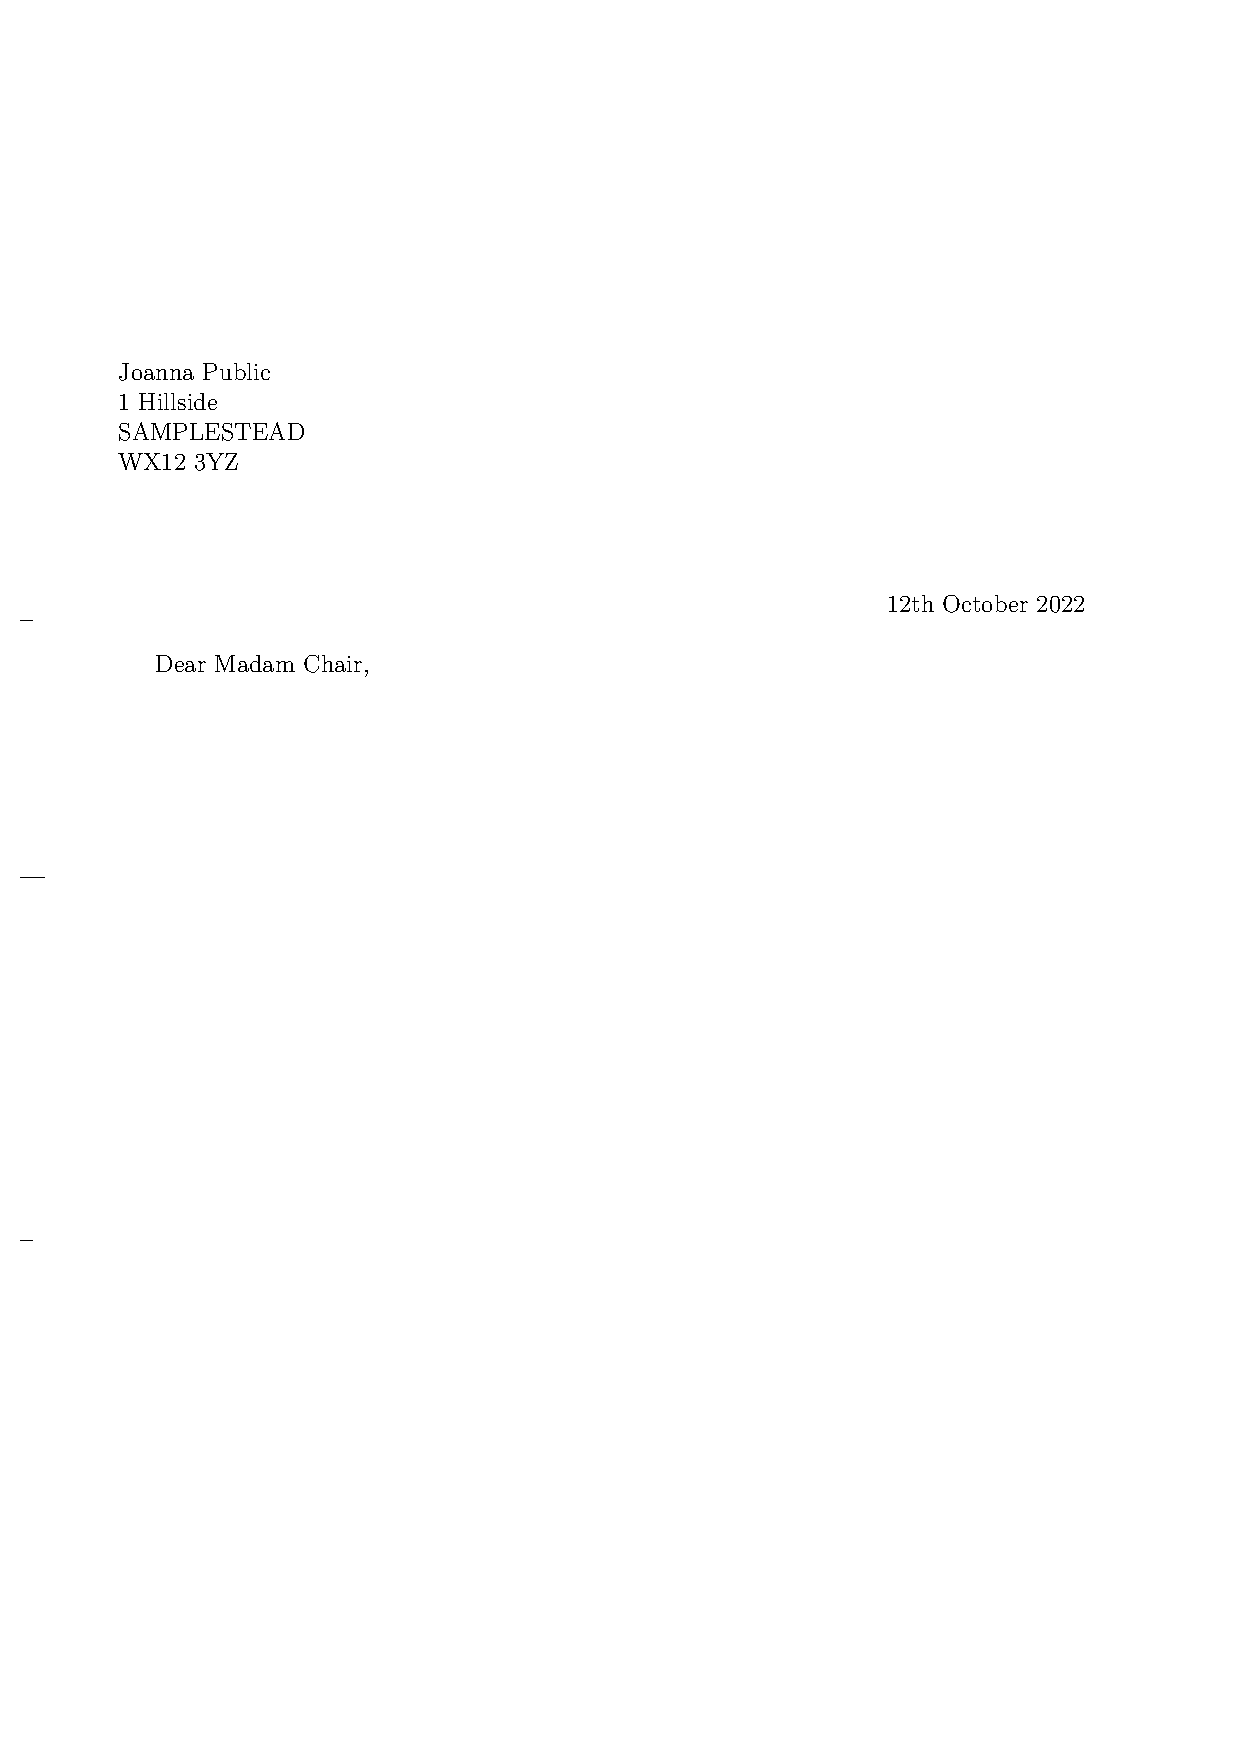
\includegraphics[width=.4\textwidth]{letter-example-00-en}}
    \end{captionbeside}
    \label{fig:\LabelBase.letter-00}
  \end{figure}
\end{Example}
\iffalse% Umbruchkorrekturtext
\begin{Explain}
  In the early days of computer-generated letters, a salutation was normally
  omitted, since individualised form letters were hardly possible. Today
  personalised greetings are common in mass mailings.%
\end{Explain}
\fi
%
\EndIndexGroup


\begin{Declaration}
  \Macro{closing}\Parameter{concluding text}
\end{Declaration}
The main purpose of the command \Macro{closing} is to typeset the
\PName{concluding text}\Index{closing}. This can even consist of multiple
lines. In that case, the individual lines should be separated by a double
backslash. Paragraph breaks inside the \PName{concluding text} are not
allowed.

In addition, this command also prints the content of the
\DescRef{\LabelBase.variable.signature} variable. You can find more
information about the signature and its configuration in
\autoref{sec:\LabelBase.closing} on
\DescPageRef{\LabelBase.variable.signature}.

\begin{Example}
  Let's extend the our example with a few lines of text and a closing phrase:
  \lstinputcode[xleftmargin=1em]{letter-example-01-en.tex}
  This will result in a the letter shown in \autoref{fig:\LabelBase.letter-01}.
  \begin{figure}
    \setcapindent{0pt}%
    \begin{captionbeside}[{Example: letter with recipient, opening, text, and
        closing}]{%
        result of a short letter with recipient, opening, text, and closing
        % The refernce to DIN-letters in the German guide isn't relevant for
        % English-language letters
        (the date is set by default)}[l]
      \frame{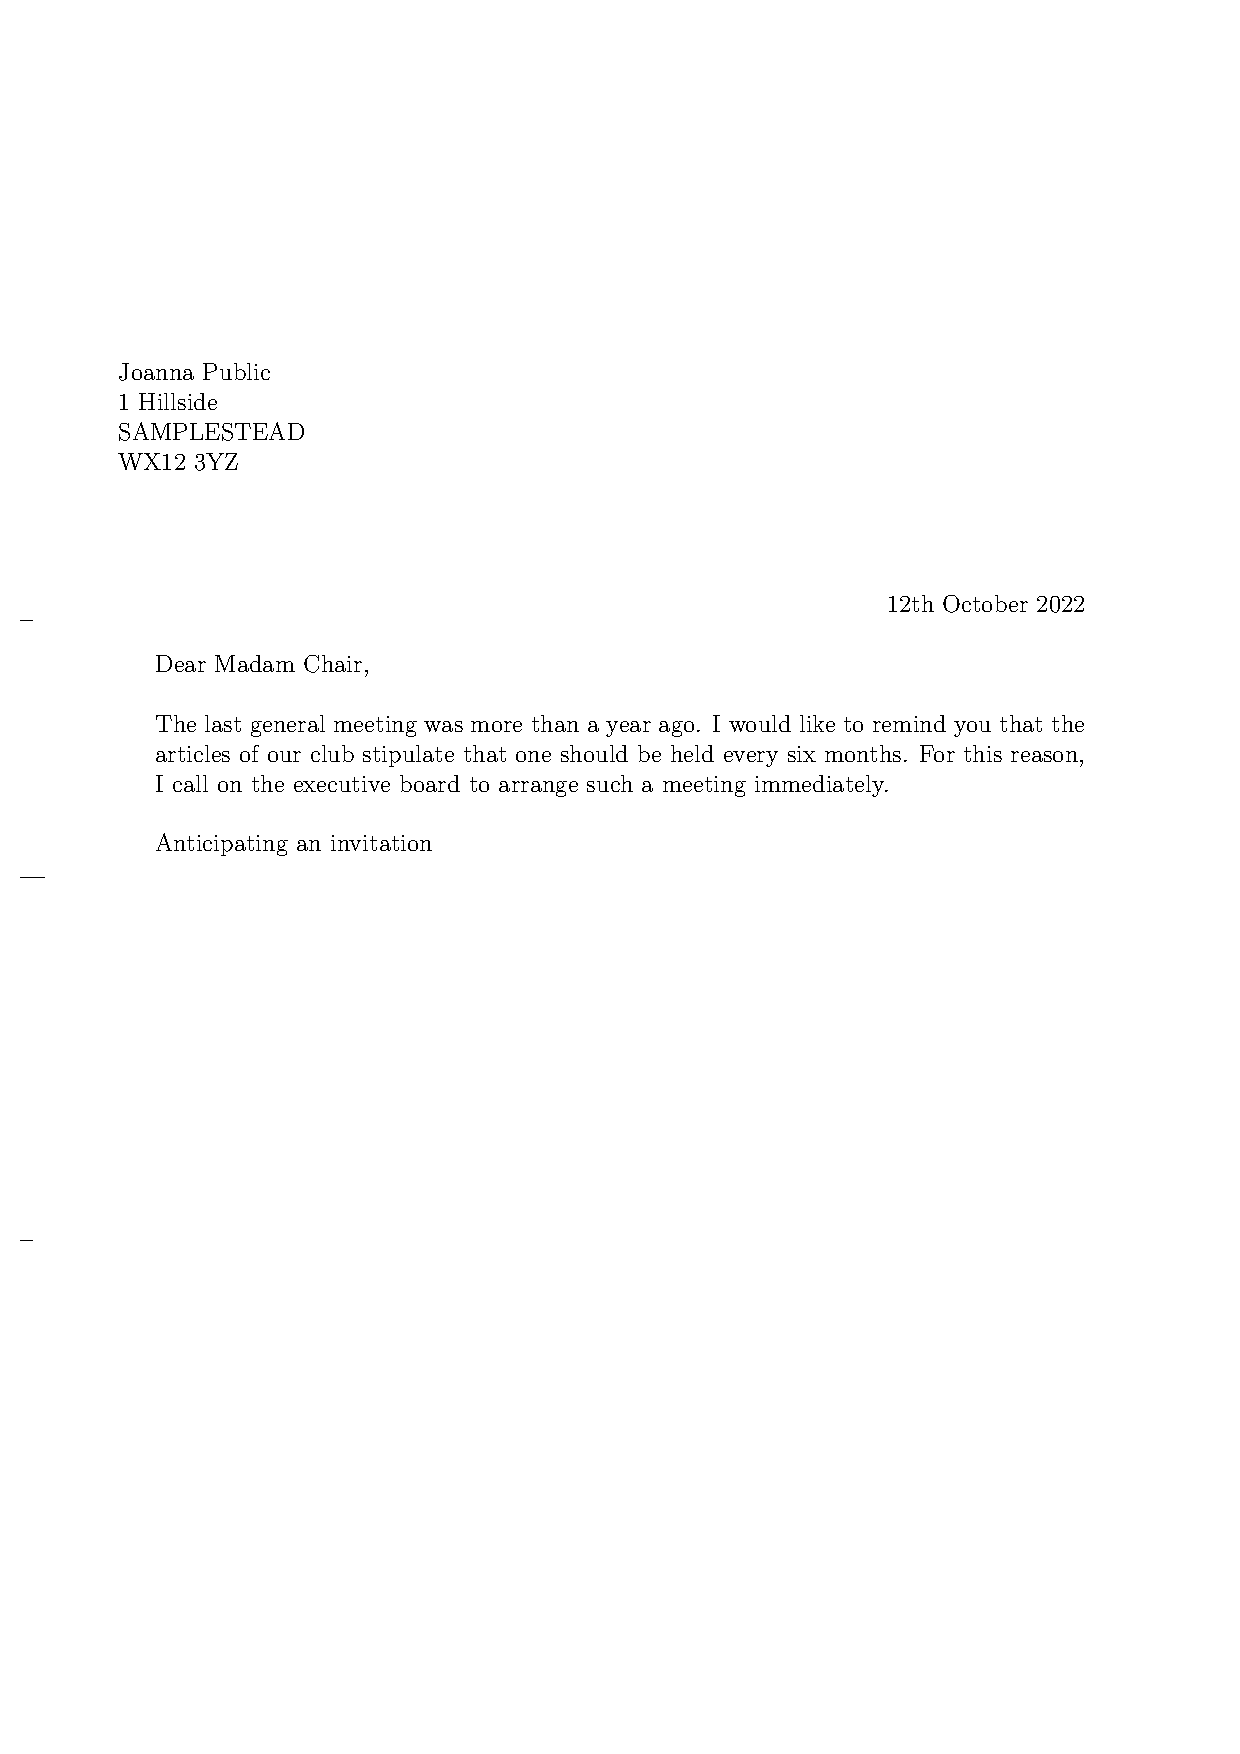
\includegraphics[width=.4\textwidth]{letter-example-01-en}}
    \end{captionbeside}
    \label{fig:\LabelBase.letter-01}
  \end{figure}
\end{Example}
%
\EndIndexGroup

\begin{Declaration}
  \Macro{ps}
\end{Declaration}%
This instruction merely switches to the postscript. To do so, a new paragraph
begins, and a vertical gap\,---\,usually below the signature\,---\,is
inserted. The \Macro{ps} text can be followed by any text. If you want the
postscript to be introduced with the acronym ``PS:'', which in most current
usage is written without full stops, you have to type this yourself. This
abbreviation is printed neither automatically nor optionally by the
\Class{scrlttr2} class.

\begin{Example}
  The sample letter with the addition of a postscript
  \lstinputcode[xleftmargin=1em]{letter-example-02-en.tex}
  results in \autoref{fig:\LabelBase.letter-02}.
  \begin{figure}
    \setcapindent{0pt}%
    \begin{captionbeside}[{Example: letter with recipient, opening, text,
        closing, and postscript}]{%
        result of a short letter with recipient, opening, text, closing, and
        postscript (the date is set by default)}[l]
      \frame{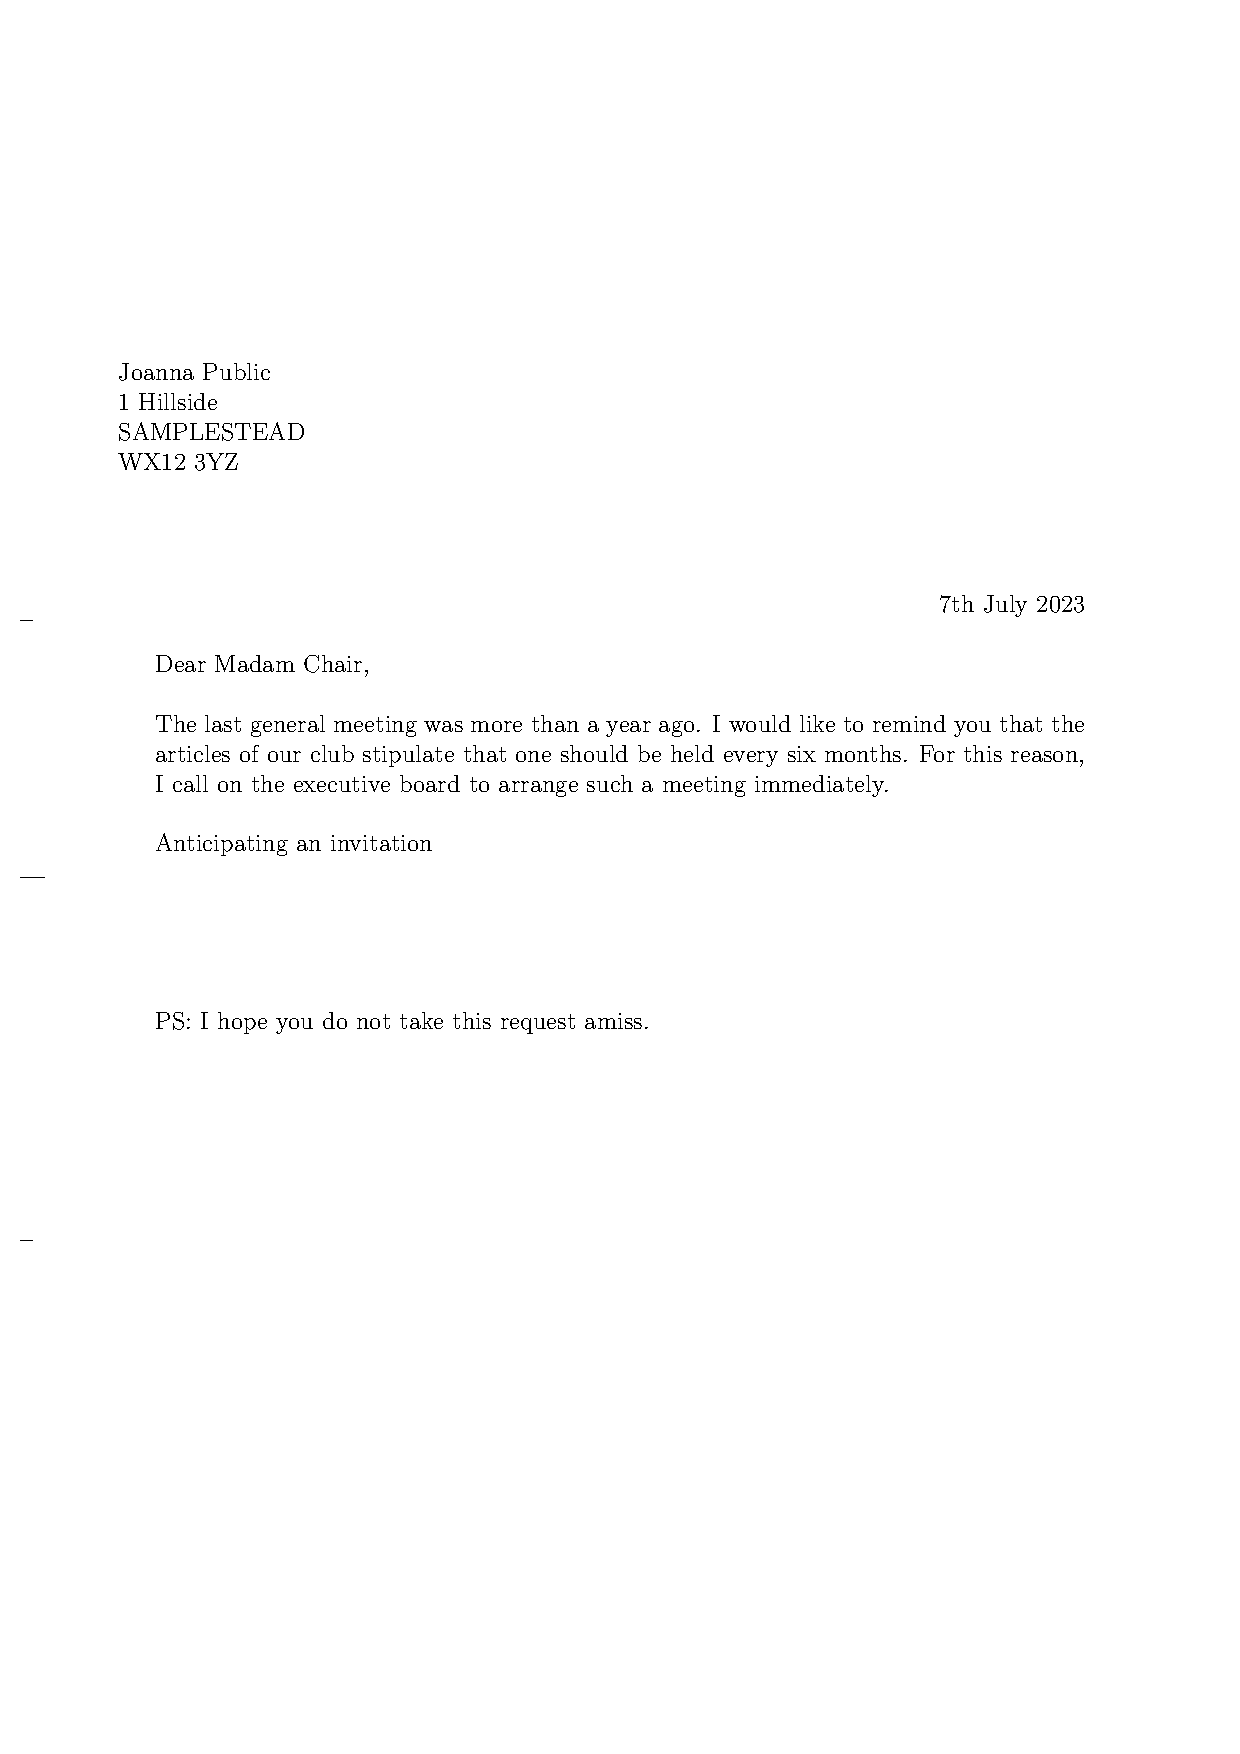
\includegraphics[width=.4\textwidth]{letter-example-02-en}}
    \end{captionbeside}
    \label{fig:\LabelBase.letter-02}
  \end{figure}
\end{Example}

\begin{Explain}
  When letters were written still by hand, it was quite common to use a
  postscript because this was the only way to add information which had been
  forgotten in the main part of the letter. For letters written with \LaTeX{},
  of course, you can easily insert additional lines. Nevertheless, postscripts
  remain popular. They can be useful to emphasize important points once more,
  or even to mention the less important matters.
\end{Explain}
%
\EndIndexGroup


\begin{Declaration}
  \Macro{cc}\Parameter{distribution list}%
  \Variable{ccseparator}%
\end{Declaration}
You can print a \PName{distribution list}\Index{recipient>additional}%
\Index{distribution list}\Index{carbon copy} with the \Macro{cc} command. The
command takes the \PName{distribution list} as its argument. If the
\PName{name} of the variable
\Variable{ccseparator}\Index{separator}\Index{delimiter} is not empty, the
\PName{name} and \PName{content} of this variable are inserted before the
\PName{distribution list}. In this case, the \PName{distribution list} will be
indented appropriately. If the individual entries are to be printed one below
the other, they can be separated by a double backslash.
\begin{Example}
  This time, the sample letter should go not only to the chairman but also to
  all club members:
  \lstinputcode[xleftmargin=1em]{letter-example-03-en.tex}%
  The result is shown in \autoref{fig:\LabelBase.letter-03}.
  \begin{figure}
    \setcapindent{0pt}%
    \begin{captionbeside}[{Example: letter with recipient, opening, text,
        closing, postscript, and distribution list}]{%
        result of a short letter with recipient, opening, text, closing,
        postscript, and distribution list (the date is set by default)}[l]
      \frame{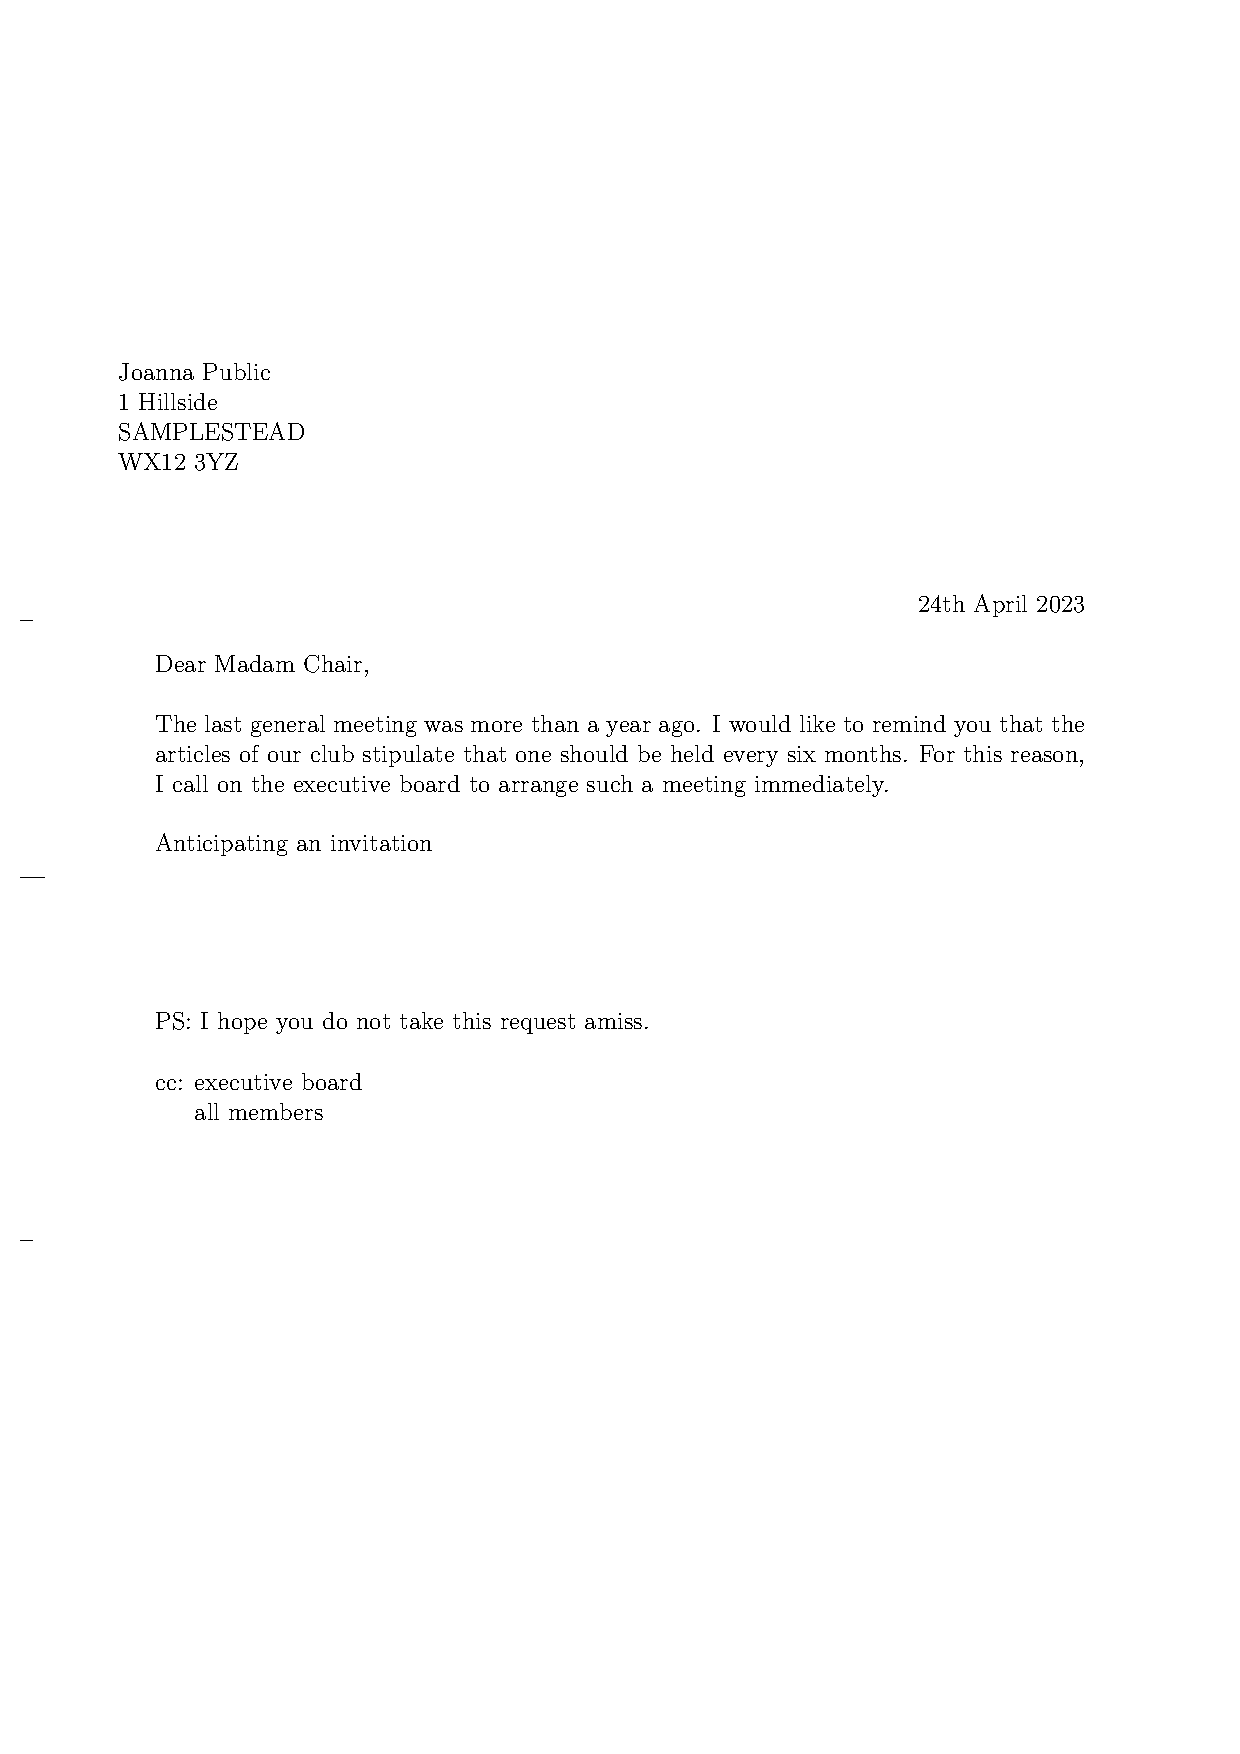
\includegraphics[width=.4\textwidth]{letter-example-03-en}}
    \end{captionbeside}
    \label{fig:\LabelBase.letter-03}
  \end{figure}
\end{Example}
A vertical gap is inserted automatically before the distribution list.%
%
\EndIndexGroup


\begin{Declaration}
  \Macro{encl}\Parameter{enclosures}%
  \Variable{enclseparator}%
\end{Declaration}
The \PName{enclosures} have the same structure as the distribution list. The
only difference is that the list of enclosures begins with the name and
content of the \Variable{enclseparator}\Index{separator}\Index{delimiter}
variable.
\begin{Example}
  To the sample letter we will attach an excerpt from the club's articles of
  association. These will be added as an enclosure. Because there is only one
  enclosure, we change the description title accordingly:
  \lstinputcode[xleftmargin=1em]{letter-example-04-en.tex}
  This will result in \autoref{fig:\LabelBase.letter-04}.
  \begin{figure}
    \setcapindent{0pt}%
    \begin{captionbeside}[{Example: letter with recipient, opening, text,
        closing, postscript, distribution list, and enclosure}]{%
        result of a short letter with recipient, opening, text, closing,
        postscript, distribution list, and enclosure (the date is set by
        default)}[l]
      \frame{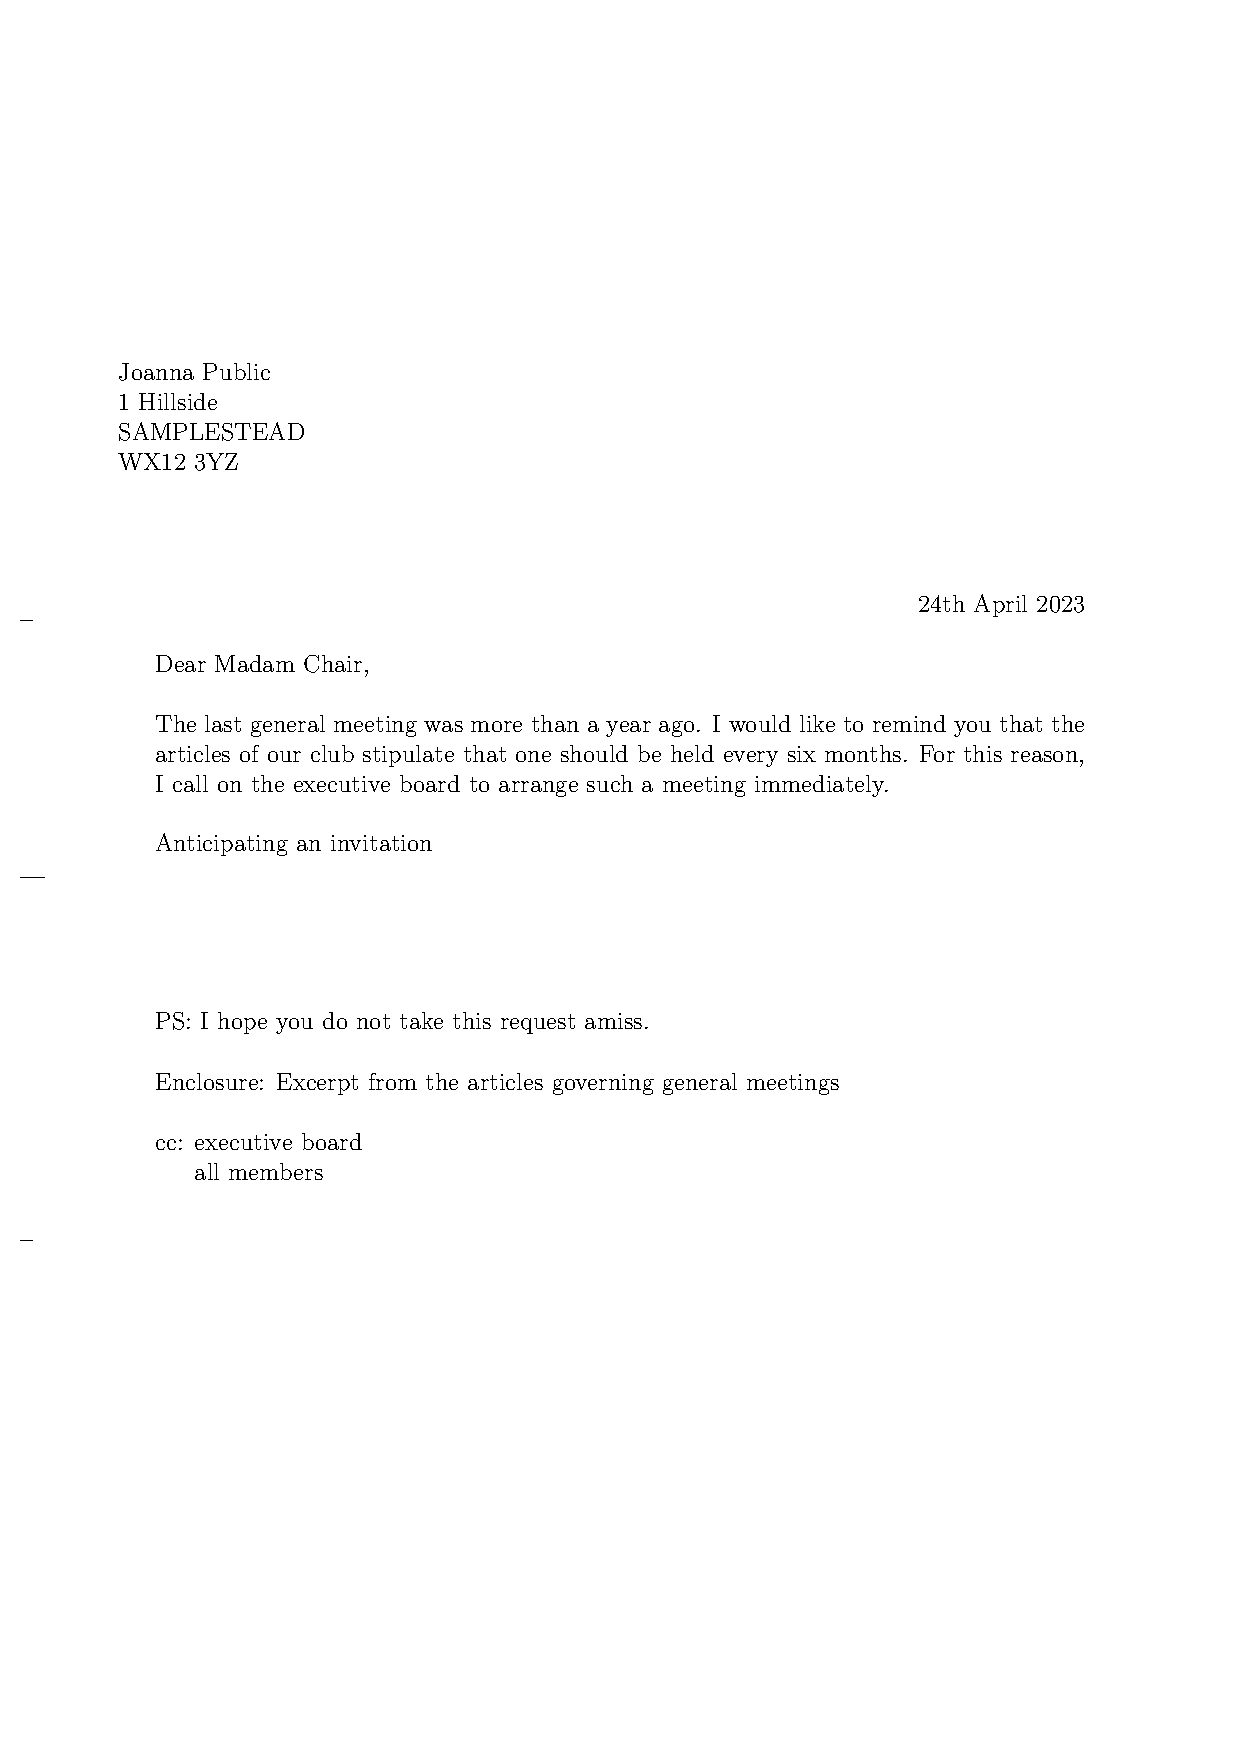
\includegraphics[width=.4\textwidth]{letter-example-04-en}}
    \end{captionbeside}
    \label{fig:\LabelBase.letter-04}
  \end{figure}
\end{Example}
%
\EndIndexGroup
%
\EndIndexGroup


\LoadCommonFile{fontsize} % \section{Choosing the Document Font Size}

\LoadCommonFile{textmarkup} % \section{Text Markup}

\section{Letterhead Page}
\seclabel{firstpage}
\BeginIndexGroup
\BeginIndex{}{letterhead page}%

The letterhead page is the first page of, and therefore the signpost for, each
letter. In a business context, the paper for this page is often preprinted
stationery containing elements such as a header with the sender's information
and logo. This header itself is also known as a letterhead. \KOMAScript{} lets
you position these elements freely, and so you can not only replicate the
letterhead page directly but also fill in the required fields instantaneously.
This free positioning is achieved with pseudo-lengths (see
\autoref{sec:\LabelBase.pseudoLength} starting on
\autopageref{sec:\LabelBase.pseudoLength}). You can find a schematic
representation of the letterhead page and the variables used for it in
\autoref{fig:\LabelBase.variables}. The names of the variables are printed in
bold to better distinguish the commands from their arguments.

Subsequent pages\Index{page>subsequent}\Index{subsequent pages} should be
distinguished from the letterhead page. For the purposes of this manual,
subsequent pages are all pages of a letter except the first one.

\begin{figure}
  \centering
  \tikzset{x=.56mm,y=-.56mm}
  \tiny
  % ======================================================================
% variables-tikz.tex
% Copyright (c) Markus Kohm, 2005-2022
%
% This file is part of the LaTeX2e KOMA-Script bundle.
%
% This work may be distributed and/or modified under the conditions of
% the LaTeX Project Public License, version 1.3c of the license.
% The latest version of this license is in
%   http://www.latex-project.org/lppl.txt
% and version 1.3c or later is part of all distributions of LaTeX 
% version 2005/12/01 or later and of this work.
%
% This work has the LPPL maintenance status "author-maintained".
%
% The Current Maintainer and author of this work is Markus Kohm.
%
% This work consists of all files listed in MANIFEST.md.
% ======================================================================
%
% Generation of plength figures at scrlttr2 chapter of the KOMA-Script
% guide
%
% Maintained by Markus Kohm
% Original metapost source by Stephan Hennig
% Original TikZ source by Marei Peischl
%
% ======================================================================

\KOMAProvidesFile{variables-tikz.tex}%
                 [$Date: 2022-06-05 12:40:11 +0200 (So, 05. Jun 2022) $
                  KOMA-Script guide (figure in scrlttr2.tex)]
                 
\ExplSyntaxOn
\prop_if_exist:NF \l_this_plength_description_prop {
  \prop_new:N \l_this_plength_description_prop
}
\prop_set_from_keyval:Nn \l_this_plength_description_prop {
  firsthead=\Multi{\DescRef{scrlttr2.variable.firsthead}\\
    \DescRef{scrlttr2.variable.fromname}\and
    \DescRef{scrlttr2.variable.fromaddress}\and
    \DescRef{scrlttr2.variable.fromphone}\and
    \DescRef{scrlttr2.variable.fromfax}\and
    \DescRef{scrlttr2.variable.fromemail}\and
    \DescRef{scrlttr2.variable.fromurl}},
  firstfoot=\DescRef{scrlttr2.variable.firstfoot},
  backaddress =\DescRef{scrlttr2.variable.backaddress},
  specialmail=\DescRef{scrlttr2.variable.specialmail},
  refline=\Multi{\DescRef{scrlttr2.variable.yourref}\and
    \DescRef{scrlttr2.variable.yourmail}\and
    \DescRef{scrlttr2.variable.myref}\and
    \DescRef{scrlttr2.variable.customer}\and
    \DescRef{scrlttr2.variable.invoice}\and
    \DescRef{scrlttr2.variable.place}\and
    \DescRef{scrlttr2.variable.date}},
  title=\DescRef{scrlttr2.variable.title},
  subject=\DescRef{scrlttr2.variable.subject},
  signature=\DescRef{scrlttr2.variable.signature},
  location= \DescRef{scrlttr2.variable.location},
  toaddr=\Macro{begin}\PParameter{\DescRef{scrlttr2.env.letter}}\Parameter{\toaddrname},
  opening=\DescRef{scrlttr2.cmd.opening}\Parameter{\openingargumentname},
  body=\desc\letterbodyname,
  closing=\DescRef{scrlttr2.cmd.closing}\Parameter{\closingargumentname},
}

\prop_if_exist:NF \l_this_plength_var_prop {
  \prop_new:N \l_this_plength_var_prop
}

\prop_set_from_keyval:Nn \l_this_plength_var_prop {
  ticksize=1,
  textwidth= 147,
  textheight= 209.4,
  evensidemargin= 6.1,
  oddsidemargin = 6.1,
  paperwidth = 210,
  paperheight = 297,
  baselineskip = .9\baselineskip, %3.86607,
  headheight     =  6,
  headsep        =7.2,
  footskip       =16.73,
  foldmarkhpos = 3.5,
  tfoldmarkvpos = 105,
  bfoldmarkvpos = 210,
  tfoldmarklength = 2,
  pfoldmarklength = 4,
  bfoldmarklength = 2,
  toaddrvpos = 45,
  refvpos = 98.5,
  refaftervskip = \UseVar{baselineskip},
  toaddrhpos = 20,
  toaddrwidth = 85,
  toaddrheight = 40,
  toaddrindent = 6,
  specialmailwidth = 50,
  specialmailrightindent = 4,
  specialmailheight = \UseVar{baselineskip},
  locwidth = 37.5,
  backaddrheight = 5,
  firstheadvpos = 8,
  firstheadwidth = \UseVar{paperwidth} - 2 * \UseVar{toaddrhpos},
  firstfootwidth = \UseVar{firstheadwidth},
  firstfootvpos =  16.58 + \UseVar{headheight} + \UseVar{headsep} + \UseVar{textheight} + \UseVar{footskip},
  refwidth = 0,
  sigindent = 0,
  toaddrindent =0,
  sigbeforevskip = 2*\UseVar{baselineskip},
  firstheadhpos = 0.5* \UseVar{paperwidth}-.5*\UseVar{firstheadwidth},
  firstheadheight = 5*\UseVar{baselineskip},
  firstfoothpos = 0.5*(\UseVar{paperwidth}-\UseVar{firstfootwidth}),
  firstfootheight = 3*\UseVar{baselineskip},
  fromrulewidth = 0.5 * \UseVar{firstheadwidth},
  lochpos = \UseVar{paperwidth}-\UseVar{toaddrhpos}-\UseVar{locwidth},
  refhpos = 25.40+\UseVar{oddsidemargin},
  text = \UseVar{refhpos},
  textcenter = \UseVar{refhpos}+0.5*\UseVar{textwidth},
  refheight = 2*\UseVar{baselineskip},
  refwidth = \UseVar{textwidth},
  titlevpos = \UseVar{refvpos}+\UseVar{refheight}+\UseVar{refaftervskip},
  titlewidth = 90,
  titleheight = 1.2*\UseVar{baselineskip},
  subjectvpos = \UseVar{titlevpos}+\UseVar{titleheight}+1*\UseVar{baselineskip},
  subjectwidth = 80,
  subjectheight = \UseVar{baselineskip},
  openingvpos = \UseVar{subjectvpos}+\UseVar{subjectheight}+2*\UseVar{baselineskip},
  openingwidth = 60,
  openingheight = \UseVar{baselineskip},
  bodyvpos = \UseVar{openingvpos}+\UseVar{openingheight}+\UseVar{baselineskip},
  bodywidth = \UseVar{textwidth},
  bodyheight = 6*\UseVar{baselineskip},
  typeareabottom = \UseVar{firstfootvpos}-\UseVar{footskip},
  sigvpos = \UseVar{bodyvpos}+\UseVar{bodyheight}+\UseVar{baselineskip},
  sigwidth = 50,
  sigheight = \UseVar{baselineskip},
  locvpos = \UseVar{toaddrvpos},
  locheight = \UseVar{toaddrheight},
}
\def\UseVar#1{
  \fp_eval:n {\prop_item:Nn \l_this_plength_var_prop {#1}}
}

\def\UseDesc#1{
  \prop_item:Nn \l_this_plength_description_prop {#1}
}

\ExplSyntaxOff

\def\desc{\itshape}

\providecommand*{\Multi}[1]{%
  {\def\and{, }%
    \begin{tabular}{@{}l@{}}
      #1
    \end{tabular}
  }%
}

\begin{tikzpicture}[fill=black!20]
  \draw (0,0)rectangle (\UseVar{paperwidth},\UseVar{paperheight});
  
  \filldraw(\UseVar{firstheadhpos},\UseVar{firstheadvpos})rectangle node{\UseDesc{firsthead}}+(\UseVar{firstheadwidth},\UseVar{firstheadheight});
  
  \filldraw(\UseVar{toaddrhpos},\UseVar{toaddrvpos}) rectangle
  node {\UseDesc{backaddress}}
  +(\UseVar{toaddrwidth},\UseVar{backaddrheight});
  
  \filldraw(\UseVar{toaddrhpos}+.5*\UseVar{toaddrwidth}-\UseVar{specialmailrightindent},\UseVar{toaddrvpos}+\UseVar{backaddrheight}) rectangle
  node {\UseDesc{specialmail}}
  +(.5*\UseVar{toaddrwidth},\UseVar{specialmailheight});
  
  \filldraw(\UseVar{toaddrhpos}+\UseVar{toaddrindent},\UseVar{toaddrvpos}+\UseVar{backaddrheight}+\UseVar{specialmailheight})
  rectangle node {\UseDesc{toaddr}}
  +(\UseVar{toaddrwidth}-2*\UseVar{toaddrindent},\UseVar{toaddrheight}-\UseVar{backaddrheight}-\UseVar{specialmailheight});
  
  \draw(\UseVar{toaddrhpos},\UseVar{toaddrvpos})rectangle+(\UseVar{toaddrwidth},\UseVar{toaddrheight});
  
  \filldraw (\UseVar{refhpos},\UseVar{refvpos})rectangle node{\UseDesc{refline}}
  +(\UseVar{refwidth},\UseVar{refheight});
  
  \filldraw (\UseVar{textcenter}-.5*\UseVar{titlewidth},\UseVar{titlevpos})rectangle node{\UseDesc{title}}
  +(\UseVar{titlewidth},\UseVar{titleheight});
  
  \filldraw (\UseVar{text},\UseVar{subjectvpos})rectangle node{\UseDesc{subject}}
  +(\UseVar{subjectwidth},\UseVar{subjectheight});
  
  \filldraw (\UseVar{text},\UseVar{openingvpos})rectangle node{\UseDesc{opening}}
  +(\UseVar{openingwidth},\UseVar{openingheight});
  
  \filldraw (\UseVar{text},\UseVar{bodyvpos})rectangle node{\UseDesc{body}}
  +(\UseVar{bodywidth},\UseVar{bodyheight});
  
  \filldraw (\UseVar{text}+\UseVar{sigindent},\UseVar{sigvpos})rectangle node{\UseDesc{closing}}
  +(\UseVar{sigwidth},\UseVar{sigheight});
  
  \filldraw (\UseVar{text}+\UseVar{sigindent}+.1*\UseVar{sigwidth},\UseVar{sigvpos}+\UseVar{sigheight}+\UseVar{sigbeforevskip})rectangle node{\UseDesc{signature}}
  +(.8*\UseVar{sigwidth},\UseVar{sigheight});
  
  \filldraw (\UseVar{lochpos},\UseVar{locvpos}) rectangle node{\UseDesc{location}}+(\UseVar{locwidth},\UseVar{locheight});
  
  \filldraw (\UseVar{firstfoothpos},\UseVar{firstfootvpos}) rectangle node{\UseDesc{firstfoot}} +(\UseVar{firstfootwidth},\UseVar{firstfootheight});
  
  \draw[thick] (\UseVar{foldmarkhpos},\UseVar{tfoldmarkvpos}) --+(\UseVar{tfoldmarklength},0);
  \draw[thick] (\UseVar{foldmarkhpos},.5*\UseVar{paperheight}) --+(\UseVar{pfoldmarklength},0);
  \draw[thick] (\UseVar{foldmarkhpos},\UseVar{bfoldmarkvpos}) --+(\UseVar{bfoldmarklength},0);
\end{tikzpicture}

\endinput

%%% Local Variables: 
%%% mode: latex
%%% coding: utf-8
%%% End: 

  \caption{schematic display of the letterhead page outlining the most
    important commands and variables}
  \label{fig:\LabelBase.variables}
\end{figure}


\subsection{Fold Marks}
\seclabel{foldmarks}
\BeginIndexGroup
\BeginIndex{}{fold marks}%
\index{marks>folding|see{fold marks}}

Fold marks, or folding marks, are short horizontal lines at the left edge, and
short vertical lines at the upper edge of the paper. \KOMAScript{} currently
supports three configurable horizontal and one configurable vertical fold
marks. In addition, there is support for a hole-punch mark, or centre mark,
which cannot be shifted vertically.

\begin{Declaration}
  \OptionVName{foldmarks}{setting}
\end{Declaration}
The \Option{foldmarks} option activates or deactivates fold marks for two,
three, or four vertical divisions and one horizontal division. The individual
parts do not have to be of equal size. The positions of three of the four
horizontal marks and the single vertical mark are configurable via
pseudo-lengths (see \autoref{sec:\LabelBase.pseudoLength},
\autopageref{sec:\LabelBase.pseudoLength}).

With the \Option{foldmarks} option, you can either use the default values for
simple switches described in \autoref{tab:truefalseswitch},
\autopageref{tab:truefalseswitch} in order to activate or deactivate all
configured fold marks on the left and upper edges of the paper at once,
or\ChangedAt{v2.97e}{\Class{scrlttr2}} you can configure the individual fold
marks independently by specifying one or more letters, as listed in
\autoref{tab:\LabelBase.foldmark}. In the latter case, the fold marks are only
shown if they have not been deactivated globally with \PValue{false},
\PValue{off}, or \PValue{no}. The exact position of the fold marks is depends
on the user settings or the \File{lco} files (see
\autoref{sec:\LabelBase.lcoFile} starting on
\autopageref{sec:\LabelBase.lcoFile}). The default values are \PValue{true}
and \PValue{TBMPL}.\textnote{default}
%
\begin{table}
%  \centering
  \KOMAoptions{captions=topbeside}%
  \setcapindent{0pt}%
%  \caption
  \begin{captionbeside}{%
      Combinable values for configuring fold marks with the
      \Option{foldmarks} option%
    }[l]
    \begin{tabular}[t]{ll}
      \toprule
      \PValue{B} & activate bottom horizontal fold mark on left paper edge\\%
      \PValue{b} & deactivate bottom horizontal fold mark on left paper edge\\%
      \PValue{H} & activate all horizontal fold marks on left paper edge\\%
      \PValue{h} & deactivate all horizontal fold marks on left paper edge\\%
      \PValue{L} & activate left vertical fold mark on upper paper edge\\%
      \PValue{l} & deactivate left vertical fold mark on upper paper edge\\%
      \PValue{M} & activate middle horizontal fold mark on left paper edge\\%
      \PValue{m} & deactivate middle horizontal fold mark on left paper edge\\%
      \PValue{P} & activate hole-punch or centre mark on left paper edge\\%
      \PValue{p} & deactivate hole-punch or centre mark on left paper edge\\%
      \PValue{T} & activate top horizontal fold mark on left paper edge\\%
      \PValue{t} & deactivate top horizontal fold mark on left paper edge\\%
      \PValue{V} & activate all vertical fold marks on upper paper edge\\%
      \PValue{v} & deactivate all vertical fold marks on upper paper edge\\%
      \bottomrule
    \end{tabular}
  \end{captionbeside}
  \label{tab:\LabelBase.foldmark}
\end{table}
%
\begin{Example}
  Suppose you want to deactivate all fold marks except the hole-punch mark. If
  the default has not already been changed, you can deactivate it as follows:
\begin{lstlisting}
  \KOMAoptions{foldmarks=blmt}
\end{lstlisting}
  If there is a chance that the default has already been changed, you should
  use a safer method. This changes our example a little bit:
  \lstinputcode[xleftmargin=1em]{letter-example-07-en.tex}%
  The result is shown in \autoref{fig:\LabelBase.letter-07}.
  \begin{figure}
    \setcapindent{0pt}%
    \begin{captionbeside}[{Example: letter with recipient, opening, text,
        closing, postscript, distribution list, enclosure, and hole-punch
        mark}]{%
        result of a short letter with recipient, opening, text, closing,
        postscript, distribution list, enclosure, and hole-punch mark
        (the date is set by default)}[l]
      \frame{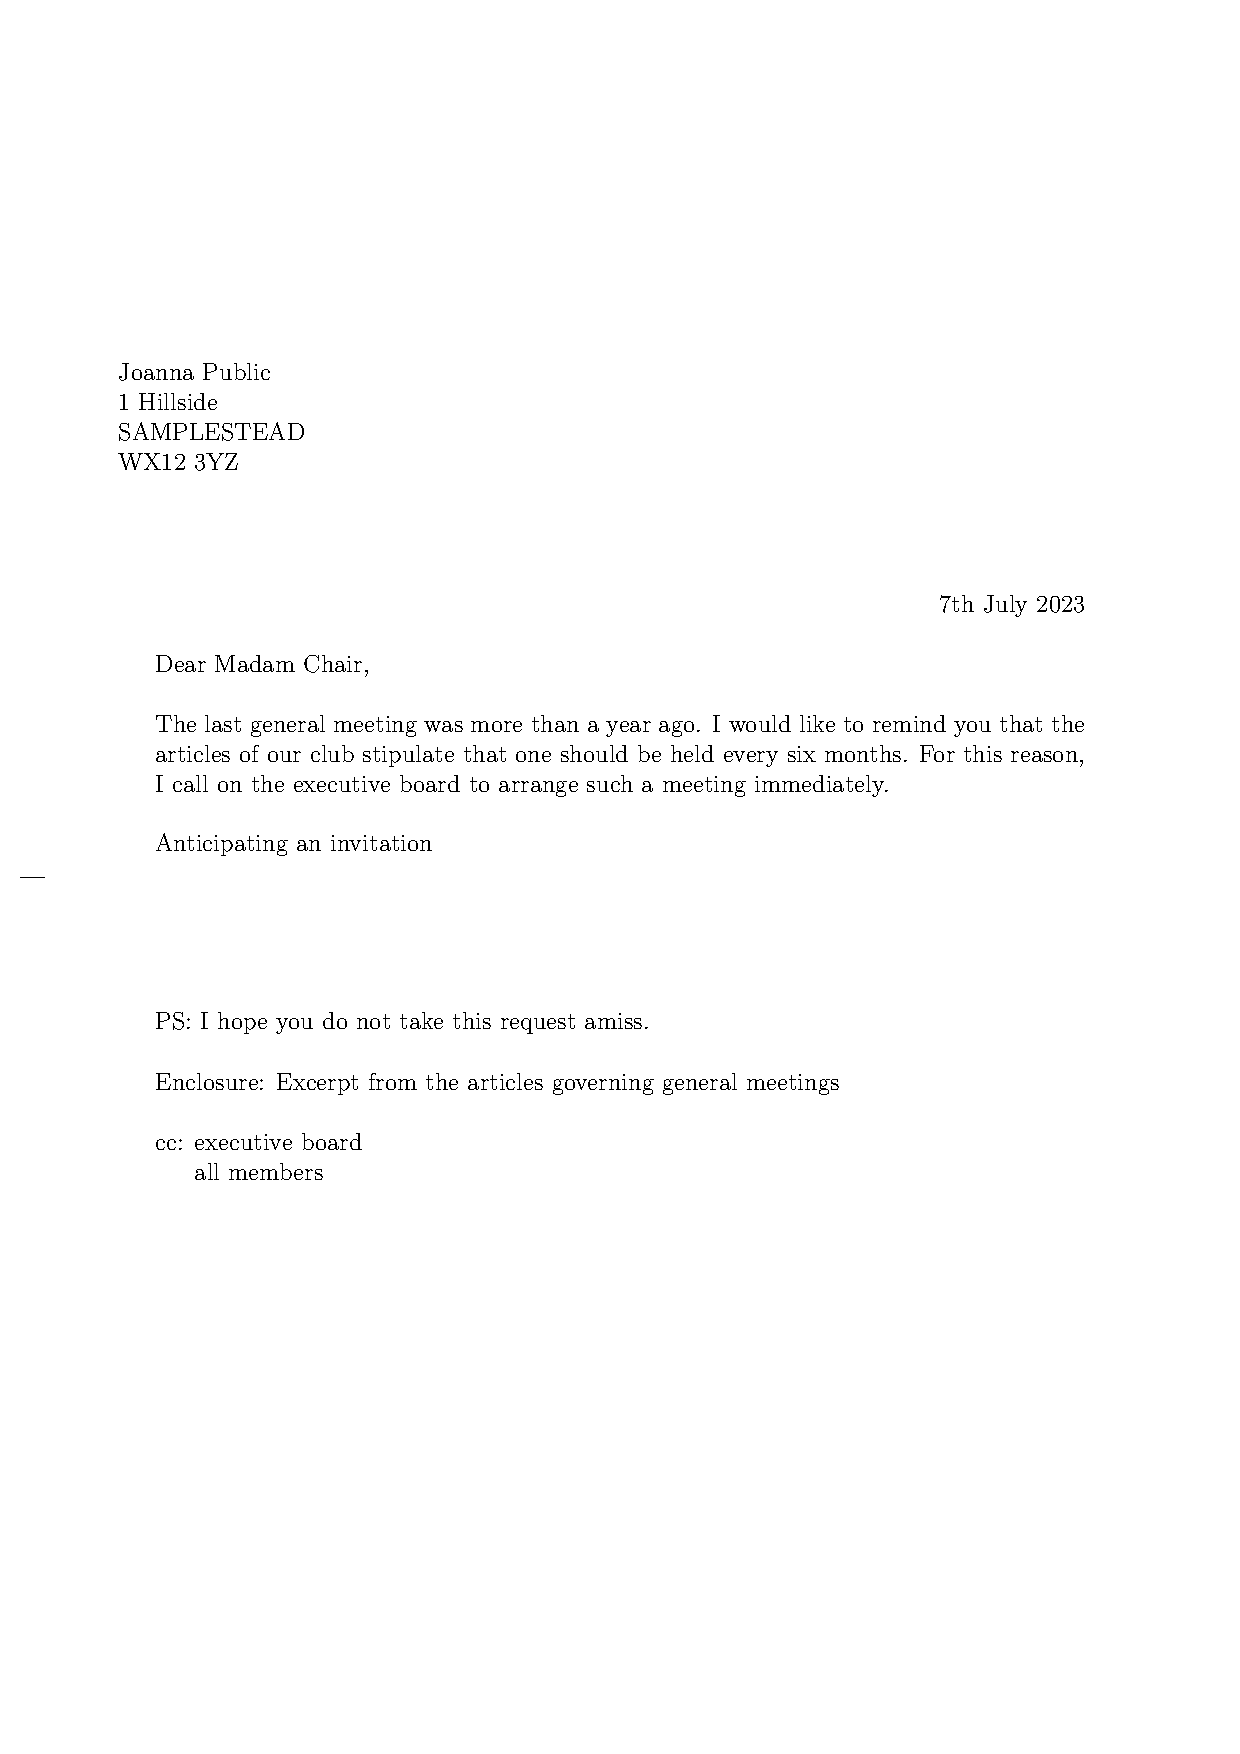
\includegraphics[width=.4\textwidth]{letter-example-07-en}}
    \end{captionbeside}
    \label{fig:\LabelBase.letter-07}
  \end{figure}
\end{Example}
\BeginIndex{FontElement}{foldmark}\LabelFontElement{foldmark}%
You\ChangedAt{v2.97c}{\Class{scrlttr2}} can change the colour of the fold mark
with the \DescRef{\LabelBase.cmd.setkomafont} and
\DescRef{\LabelBase.cmd.addtokomafont} commands (see
\autoref{sec:\LabelBase.textmarkup}, \DescPageRef{\LabelBase.cmd.setkomafont})
with the \FontElement{foldmark} element. The default is no change.%
\EndIndexGroup


\begin{Declaration}
  \PLength{tfoldmarkvpos}%
  \PLength{mfoldmarkvpos}%
  \PLength{bfoldmarkvpos}
\end{Declaration}
\KOMAScript{} recognises a total of three fold marks whose vertical position
can be configured. The distance of the top fold mark from the upper edge of
the paper is determined by the \PLength{tfoldmarkvpos} pseudo-length; the
distance of the middle fold mark, by the
\PLength{mfoldmarkvpos}\ChangedAt{v2.97e}{\Class{scrlttr2}} pseudo-length; the
distance of the bottommost fold mark, by \PLength{bfoldmarkvpos}
pseudo-length. With the addition of the hole-punch\Index{hole-punch mark} or
centre\Index{centre mark|see{hole-punch mark}} mark, there is yet a fourth
horizontal mark. This one is however always placed at the vertical centre of
the paper.
\iftrue% Umbruchkorrekturtext
There is no pseudo-length for this last mark because its vertical position is
not configurable.
\fi

The\textnote{Attention!} top and bottom fold marks do not serve to divide the
paper exactly into equal thirds. Instead, the paper should be folded with
their help such that the address field can be seen in a window envelope. The
settings are therefore different depending on the \File{lco} file chosen.
Several such files are available offering predefined formats. One format
particularly worth noting is \Option{DINmtext}. This format assumes an
envelope format of C6/5 (also known as ``C6 long''). Letters written with this
option are typically not suited for C5 or C4 envelopes.

The middle fold mark is not normally required for Western letters. In Japan,
however, a larger number of envelope formats exists, requiring one more fold
mark (see the Japanese \File{lco} files). Note that the terms ``top'',
``middle'', and ``bottom'' fold marks only represent a naming convention. In
fact, it is not required that \PLength{tfoldmarkvpos} must be smaller than
\PLength{mfoldmarkvpos}, which in turn must be smaller than
\PLength{bfoldmarkvpos}. If, though, one of the pseudo-lengths is zero, then
the corresponding fold mark will not be set even if the
\DescRef{\LabelBase.option.foldmarks}\IndexOption{foldmarks~=\PName{setting}}%
\important{\DescRef{\LabelBase.option.foldmarks}} option (see
\autoref{sec:\LabelBase.firstpage}, \DescPageRef{\LabelBase.option.foldmarks}) is
explicitly activated.
%
\EndIndexGroup


\begin{Declaration}
  \PLength{tfoldmarklength}%
  \PLength{mfoldmarklength}%
  \PLength{bfoldmarklength}%
  \PLength{pfoldmarklength}
\end{Declaration}
These\ChangedAt{v2.97e}{\Class{scrlttr2}} four pseudo-lengths determine the
lengths of the four horizontal fold marks. One\textnote{Attention!} feature is
particularly worth noting. If the length is given as zero, then the three
vertically configurable pseudo-lengths \PLength{tfoldmarklength},
\PLength{mfoldmarklength} and \PLength{bfoldmarklength} are set to 2\Unit{mm}.
The length of the hole-punch mark, \PLength{pfoldmarklength}, however, is set
to 4\Unit{mm}.%
\EndIndexGroup


\begin{Declaration}
  \PLength{foldmarkhpos}
\end{Declaration}
This pseudo-length gives the distance of all horizontal fold marks from the
left edge of the paper. Normally, this is 3.5\Unit{mm}. You\textnote{Hint!}
can change this value in your own \File{lco} file if you are using a printer
that has a wider unprintable left margin. Whether the fold marks are typeset
at all depends on the option \DescRef{\LabelBase.option.foldmarks}%
\important{\DescRef{\LabelBase.option.foldmarks}}%
\IndexOption{foldmarks~=\PName{setting}} (see
\autoref{sec:\LabelBase.firstpage}, \DescPageRef{\LabelBase.option.foldmarks}).
%
\EndIndexGroup


\begin{Declaration}
  \PLength{lfoldmarkhpos}
\end{Declaration}
In\ChangedAt{v2.97e}{\Class{scrlttr2}} addition to the horizontal fold marks,
there is also a vertical fold mark. Its distance from the left margin is set
via the \PLength{lfoldmarkhpos} pseudo-length. This fold mark is used, for
example, in Japanese Chou- or You-format envelopes if you want to use them
with A4 paper. It can also be useful for envelopes in C6 format.%
\EndIndexGroup


\begin{Declaration}
  \PLength{lfoldmarklength}
\end{Declaration}
The\ChangedAt{v2.97e}{\Class{scrlttr2}} \PLength{lfoldmarklength}
pseudo-length determines the length of the vertical fold mark. Once again, a
feature worth noting is that if the length is given as zero, a length of
4\Unit{mm} is actually used.%
\EndIndexGroup


\begin{Declaration}
  \PLength{foldmarkvpos}
\end{Declaration}
This\ChangedAt{v2.97e}{\Class{scrlttr2}} pseudo-length determines the distance of
all vertical fold marks from the upper edge of the paper. Normally this is
3.5\Unit{mm}, but\textnote{Hint!} you can change the value in your own
\File{lco} file in case your printer has a wider unprintable
top margin. Whether or not the foldmarks are actually typeset depends on the 
\DescRef{\LabelBase.option.foldmarks}%
\important{\DescRef{\LabelBase.option.foldmarks}}%
\IndexOption{foldmarks~=\PName{setting}} option (see
\autoref{sec:\LabelBase.firstpage}, \DescPageRef{\LabelBase.option.foldmarks}).
\iffree{At present there is only one vertical fold mark, called the left
  vertical fold mark.}{}%
\EndIndexGroup


\begin{Declaration}
  \PLength{foldmarkthickness}
\end{Declaration}
This\ChangedAt{v2.97c}{\Class{scrlttr2}} pseudo-length determines the
thickness of all fold marks. The default is 0.2\Unit{pt}, in other words a
very thin hairline. In\textnote{Hint!} particular, if the colour of the fold
marks is changed, this may not be enough.%
\EndIndexGroup
%
\EndIndexGroup


\subsection{Letterhead}
\seclabel{firstHead}
\BeginIndexGroup
\BeginIndex{}{letterhead}%

The term letterhead refers here to all of the information concerning the
sender that appears above the recipient's address. Normally you would expect
that this information would be set through the page-style settings. In fact,
this was the case with the old letter class, \Class{scrlettr}.
But\textnote{Attention!} \Class{scrlttr2} and \Package{scrletter} output the
letterhead independently of the page style by means of the
\DescRef{\LabelBase.cmd.opening}\IndexCmd{opening} command.
% Fuellmaterial
\iftrue%
  The letterhead is positioned absolutely, so that it is independent of the
  type area. In fact, the first page of a letter, the page that holds the
  letterhead, is set using the page style
  \DescRef{\LabelBase.pagestyle.empty}\IndexPagestyle{empty}.%
\fi
% Ende des Fuellmaterials


\begin{Declaration}
  \OptionVName{firsthead}{simple switch}
\end{Declaration}
\BeginIndex{}{letterhead}%
\BeginIndex{}{letter>header}%
The\ChangedAt{v2.97e}{\Class{scrlttr2}} letterhead is usually the topmost
element of the letterhead page. With the \Option{firsthead} option, you can
choose whether the letterhead will be typeset at all. The option accepts the
standard values for simple switches given in \autoref{tab:truefalseswitch} on
\autopageref{tab:truefalseswitch}. The default is to typeset the letterhead.%
%
\EndIndexGroup


\begin{Declaration}
  \PLength{firstheadvpos}
\end{Declaration}
The \PLength{firstheadvpos} pseudo-length gives the distance between the top
edge of the paper and the start of the letterhead. This value is set
differently in the various predefined
\File{lco} files\textnote{\File{lco} file}\Index{lco file=\File{lco} file}. A
typical value is 8\Unit{mm}.%
\EndIndexGroup


\begin{Declaration}
  \PLength{firstheadhpos}
\end{Declaration}
A positive value of the
\PLength{firstheadhpos}\ChangedAt{v3.05}{\Class{scrlttr2}} pseudo-length gives
the distance between the left edge of the paper and the start of the
letterhead. If\textnote{Attention!} the value is actually greater than or
equal to the paper width,
\Length{paperwidth}\important{\Length{paperwidth}}\IndexLength{paperwidth},
the letterhead will be centred horizontally on the letterhead paper. A
negative value gives the distance between the right edge of the paper and the
right edge of the letterhead. If the value actually less than or equal to the
negative value of the width of the paper, the letterhead is placed flush with
the left edge of the type area.

The default\textnote{Attention!} value is typically
\Length{maxdimen}\IndexLength{maxdimen}, which is the maximum allowed value of
a length. This results in horizontal centring.%
\EndIndexGroup


\begin{Declaration}
  \PLength{firstheadwidth}
\end{Declaration}
The \PLength{firstheadwidth} pseudo-length gives the width of the letterhead.
This value is set differently in the various predefined \File{lco}
files\textnote{\File{lco} file}\Index{lco file=\File{lco} file}. While this
value usually depends on the paper width and the distance between the left
edge of the paper and the recipient's address field, it was the width of the
type area in \Option{KOMAold} and has a fixed value of 170\Unit{mm} in
\Option{NF}.%
\EndIndexGroup


\begin{Declaration}
  \OptionVName{fromalign}{method}
\end{Declaration}
\BeginIndex{}{letterhead}%
\BeginIndex{}{letter>head}%
The\important{\Option{fromalign}} \Option{fromalign} option determines where
the sender information should be placed on the first page. In addition to the
various placement options in the letterhead, you also have the
ability\ChangedAt{v2.97e}{\Class{scrlttr2}} to accommodate extra sender
information\Index{extra sender information}. At the same
time\textnote{Attention!}, this option serves as a central switch to activate
or deactivate letterhead extensions. If these extensions are deactivated, some
other options will have no effect. This will be noted in the explanations of
the respective options. Available values for \Option{fromalign} are shown in
\autoref{tab:\LabelBase.fromalign}. The default value is \PValue{left}.%
%
\begin{table}
  \caption[{Available values for the \Option{fromalign} option with
    \Class{scrlttr2}}]{Available values for the \Option{fromalign} option to
    define the position of the from address in the letterhead with
    \Class{scrlttr2}}
  \label{tab:\LabelBase.fromalign}
  \begin{desctabular}
    \entry{\PValue{center}, \PValue{centered}, \PValue{middle}}{%
      Sender information is centred inside the letterhead; a logo is
      placed at the beginning of the extra sender information, if
      applicable; letterhead extensions are activated.}%
    \entry{\PValue{false}, \PValue{no}, \PValue{off}}{%
      The default design will be used for the sender information; the
      letterhead extensions are deactivated.}%
    \entry{\PValue{left}}{%
      Sender information is left-aligned in the letterhead; a logo is
      placed right-aligned, if applicable; letterhead extensions are
      activated.}%
    \entry{\PValue{locationleft}, \PValue{leftlocation}}{%
      Sender information is left-justified and uses the extra sender
      information; a logo is placed at the top of it, if applicable; the
      letterhead is automatically deactivated but can be reactivated using the
      \DescRef{\LabelBase.option.firsthead} option.}%
    \entry{\PValue{locationright}, \PValue{rightlocation},
      \PValue{location}}{%
      Sender information is right-justified and uses the extra sender
      information; a logo is placed at the top of it, if applicable; the
      letterhead is automatically deactivated but can be reactivated using the
      \DescRef{\LabelBase.option.firsthead} option.}%
    \entry{\PValue{right}}{%
      Sender information is right-justified; a logo is placed left-justified,
      if applicable; letterhead extensions are activated}%
  \end{desctabular}
\end{table}
%
\EndIndexGroup


\begin{Declaration}
  \OptionVName{fromrule}{position}%
  \Variable{fromname}%
  \Variable{fromaddress}%
\end{Declaration}
\BeginIndex{}{letterhead}%
\BeginIndex{}{letter>head}%
The\important{\Variable{fromname}} sender's name is determined by the
\Variable{fromname} variable. Its \PName{description} (see also
\autoref{tab:\LabelBase.fromTerm}, \autopageref{tab:\LabelBase.fromTerm}) is
not used in the default letterheads.

In\important{\OptionValue{fromrule}{aftername}} the extended letterhead, you
can create a horizontal rule below the sender's name with
\OptionValue{fromrule}{aftername}.
Alternatively\important{\OptionValue{fromrule}{afteraddress}} you can place
this rule below the complete sender information with
\OptionValue{fromrule}{afteraddress}. A summary of all available settings for
the rule position is shown in \autoref{tab:\LabelBase.fromrule}. The length of
this rule is determined by the
\PLength{fromrulewidth}\IndexPLength[indexmain]{fromrulewidth} pseudo-length.

\begin{table}
  \caption[{Available values for the \Option{fromrule} option with
    \Class{scrlttr2}}]{Available values for the \Option{fromrule} option for the
    position of the rule in the sender information with
    \Class{scrlttr2}}
  \label{tab:\LabelBase.fromrule}
  \begin{desctabular}
  \entry{\PValue{afteraddress}, \PValue{below}, \PValue{on}, \PValue{true},
    \PValue{yes}}{%
    rule below the sender's address}%
  \entry{\PValue{aftername}}{%
    rule directly below the sender's name}%
  \entry{\PValue{false}, \PValue{no}, \PValue{off}}{%
    no rule}%
  \end{desctabular}
\end{table}

The default\textnote{default} for the rule with the extended letterhead is
\PValue{false}. But in the standard letterhead, the rule will always be placed
below the sender's name.

The\important{\Variable{fromaddress}} sender's address follows below the name.
The \PName{content} of variable \Variable{fromaddress} determines this
address. The address \PName{description} (see also
\autoref{tab:\LabelBase.fromTerm}) is not used in the default letterheads

\BeginIndexGroup
\BeginIndex{FontElement}{fromaddress}\LabelFontElement{fromaddress}%
\BeginIndex{FontElement}{fromname}\LabelFontElement{fromname}%
\BeginIndex{FontElement}{fromrule}\LabelFontElement{fromrule}%
You can set the font used for the complete sender information with the
\FontElement{fromaddress}\IndexFontElement{fromaddress}%
\important{\FontElement{fromaddress}} element. You can define modifications to
this with the \FontElement{fromname}\IndexFontElement{fromname}%
\important{\FontElement{fromname}} element for the sender's name, and with the
\FontElement{fromrule}\IndexFontElement{fromrule}%
\important{\FontElement{fromrule}} element for the rule created with the
\Option{fromrule} option. The default setting does not change the font. For
the rule, font switching is mainly intended to change the colour of the rule,
for example to use grey instead of black. See \cite{package:xcolor} for
information about colours.%
%
\EndIndexGroup

\begin{Example}
  Now let's give the sender of our sample letter a name:
  \lstinputcode[xleftmargin=1em]{letter-example-08-en.tex}
  \begin{figure}
    \centering
    \frame{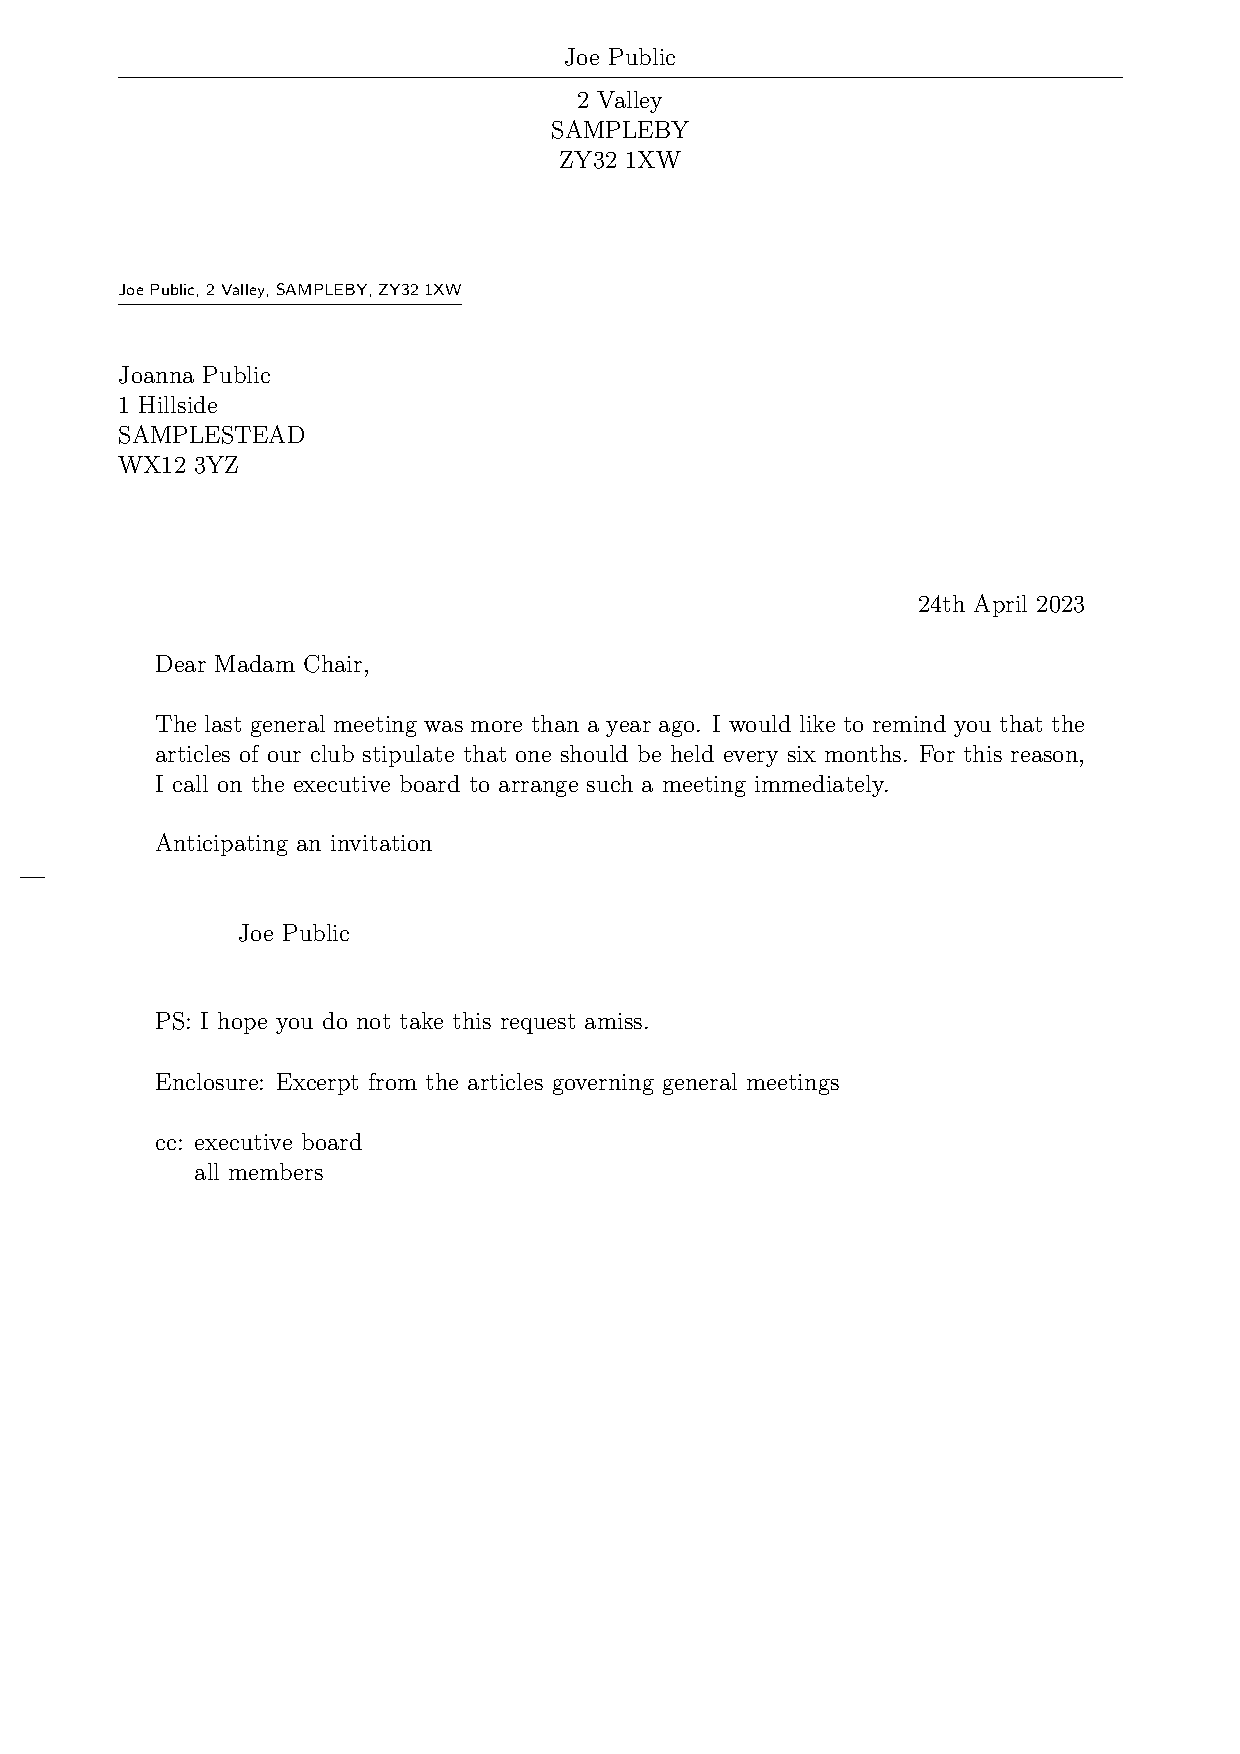
\includegraphics[width=.4\textwidth]{letter-example-08-en}}\quad
    \frame{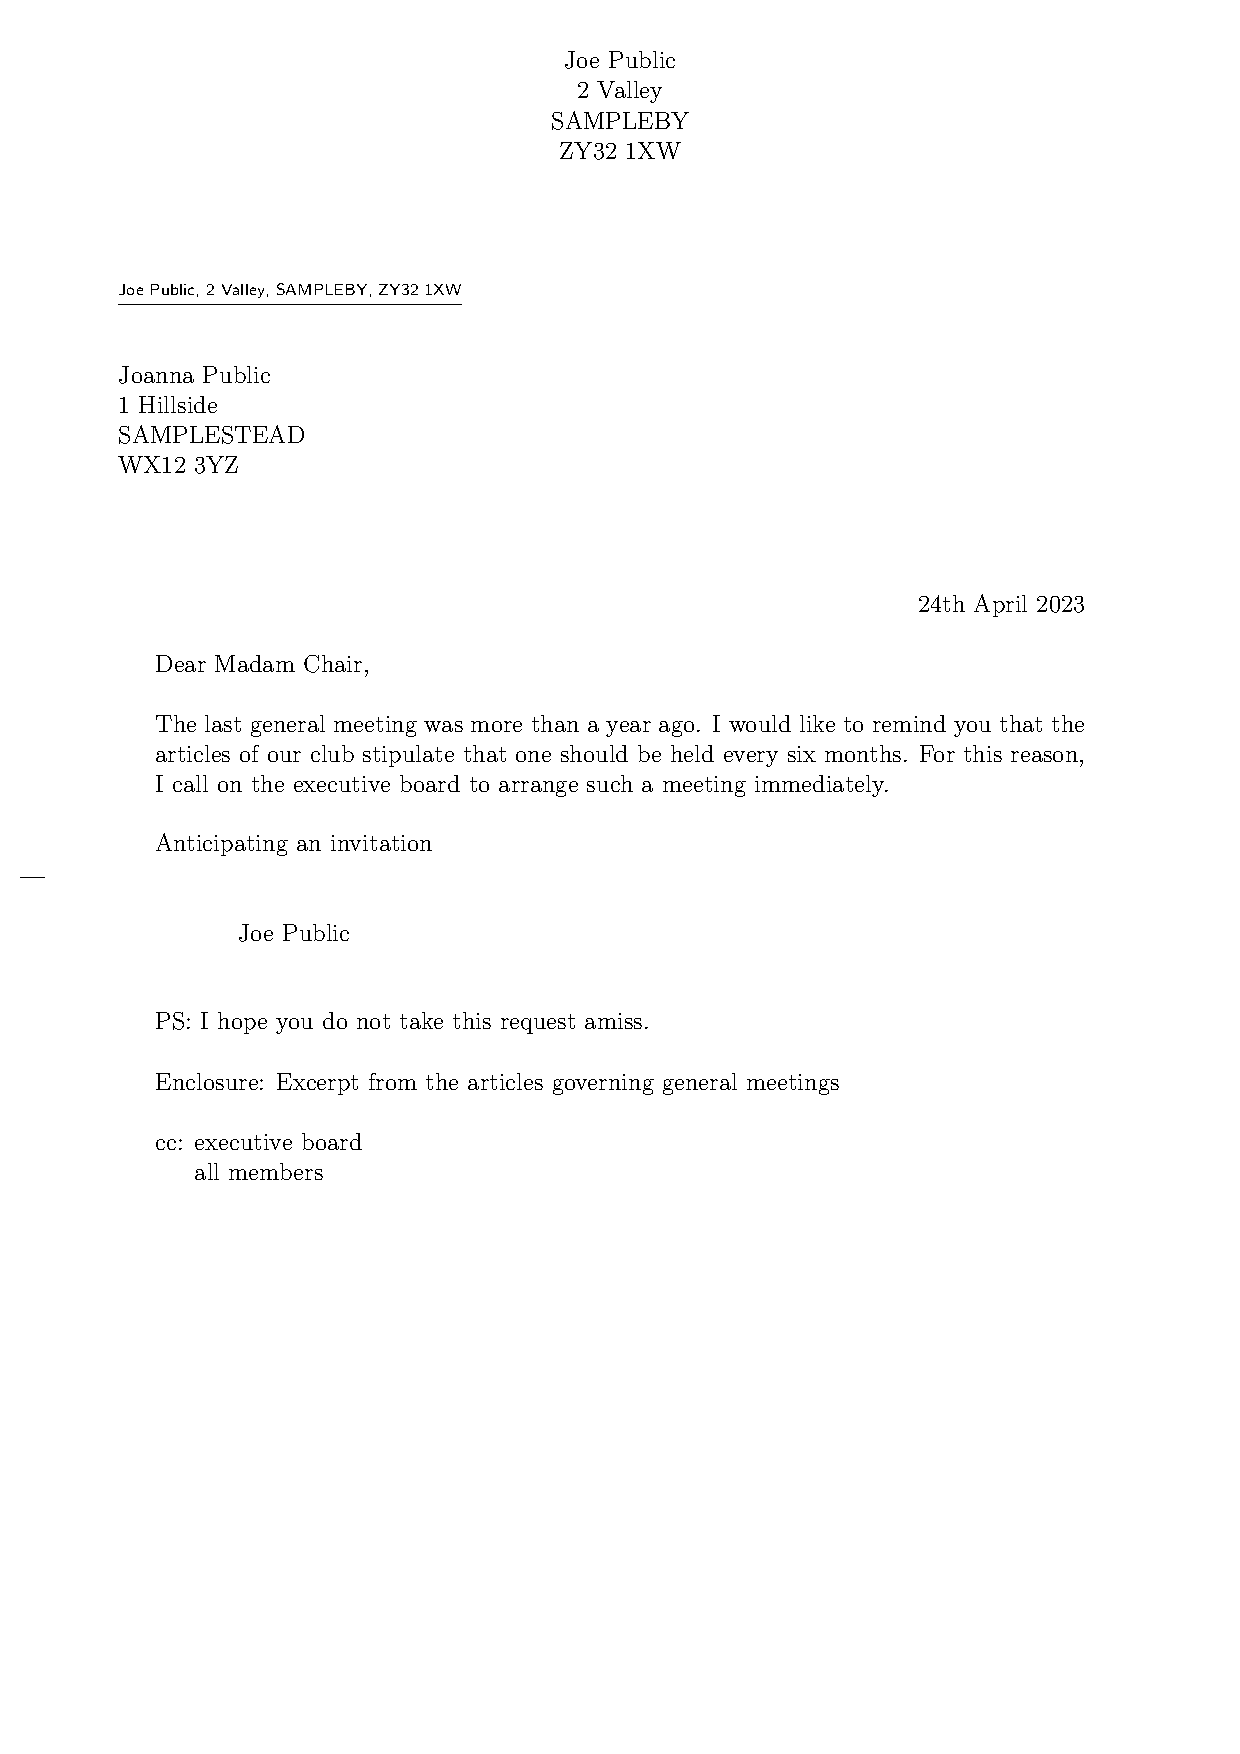
\includegraphics[width=.4\textwidth]{letter-example-09-en}}
    \caption[{Example: letter with sender, recipient, opening, text, closing,
      postscript, distribution list, and enclosure}]
    {result of a short letter with sender, recipient, opening, text, closing,
      postscript, distribution list, and enclosure (the date is set by
      default): on the left, the standard letterhead using
      \OptionValueRef{\LabelBase}{fromalign}{false}; on the right, the
      extended letterhead using \OptionValueRef{\LabelBase}{fromalign}{center}}
    \label{fig:\LabelBase.letter-08-09}
  \end{figure}
  Initially, the standard rather than the extended letterhead is used. The
  result can be seen in \autoref{fig:\LabelBase.letter-08-09} on the left. For
  comparison, the same example is shown on the right with
  \OptionValueRef{\LabelBase}{fromalign}{center} (that is, with the extended
  letterhead). You can see that this variation initially has no rule.

  For the first time, \autoref{fig:\LabelBase.letter-08-09} also shows a
  signature below the closing phrase. This is generated automatically from the
  sender's name. You can find more information about how to configure the
  signature in \autoref{sec:\LabelBase.closing}, starting on
  \autopageref{sec:\LabelBase.closing}.

  Next, the letter with the extended letterhead should use the
  \Option{fromrule} option to print a rule below the sender's name:%
  \lstinputcode[xleftmargin=1em]{letter-example-11-en.tex}%
  You can see the result on the right in
  \autoref{fig:\LabelBase.letter-10-11}. By comparison, the same example on
  the left uses the standard letterhead, which ignores the additional options.
  %
  \begin{figure}
    \centering
    \frame{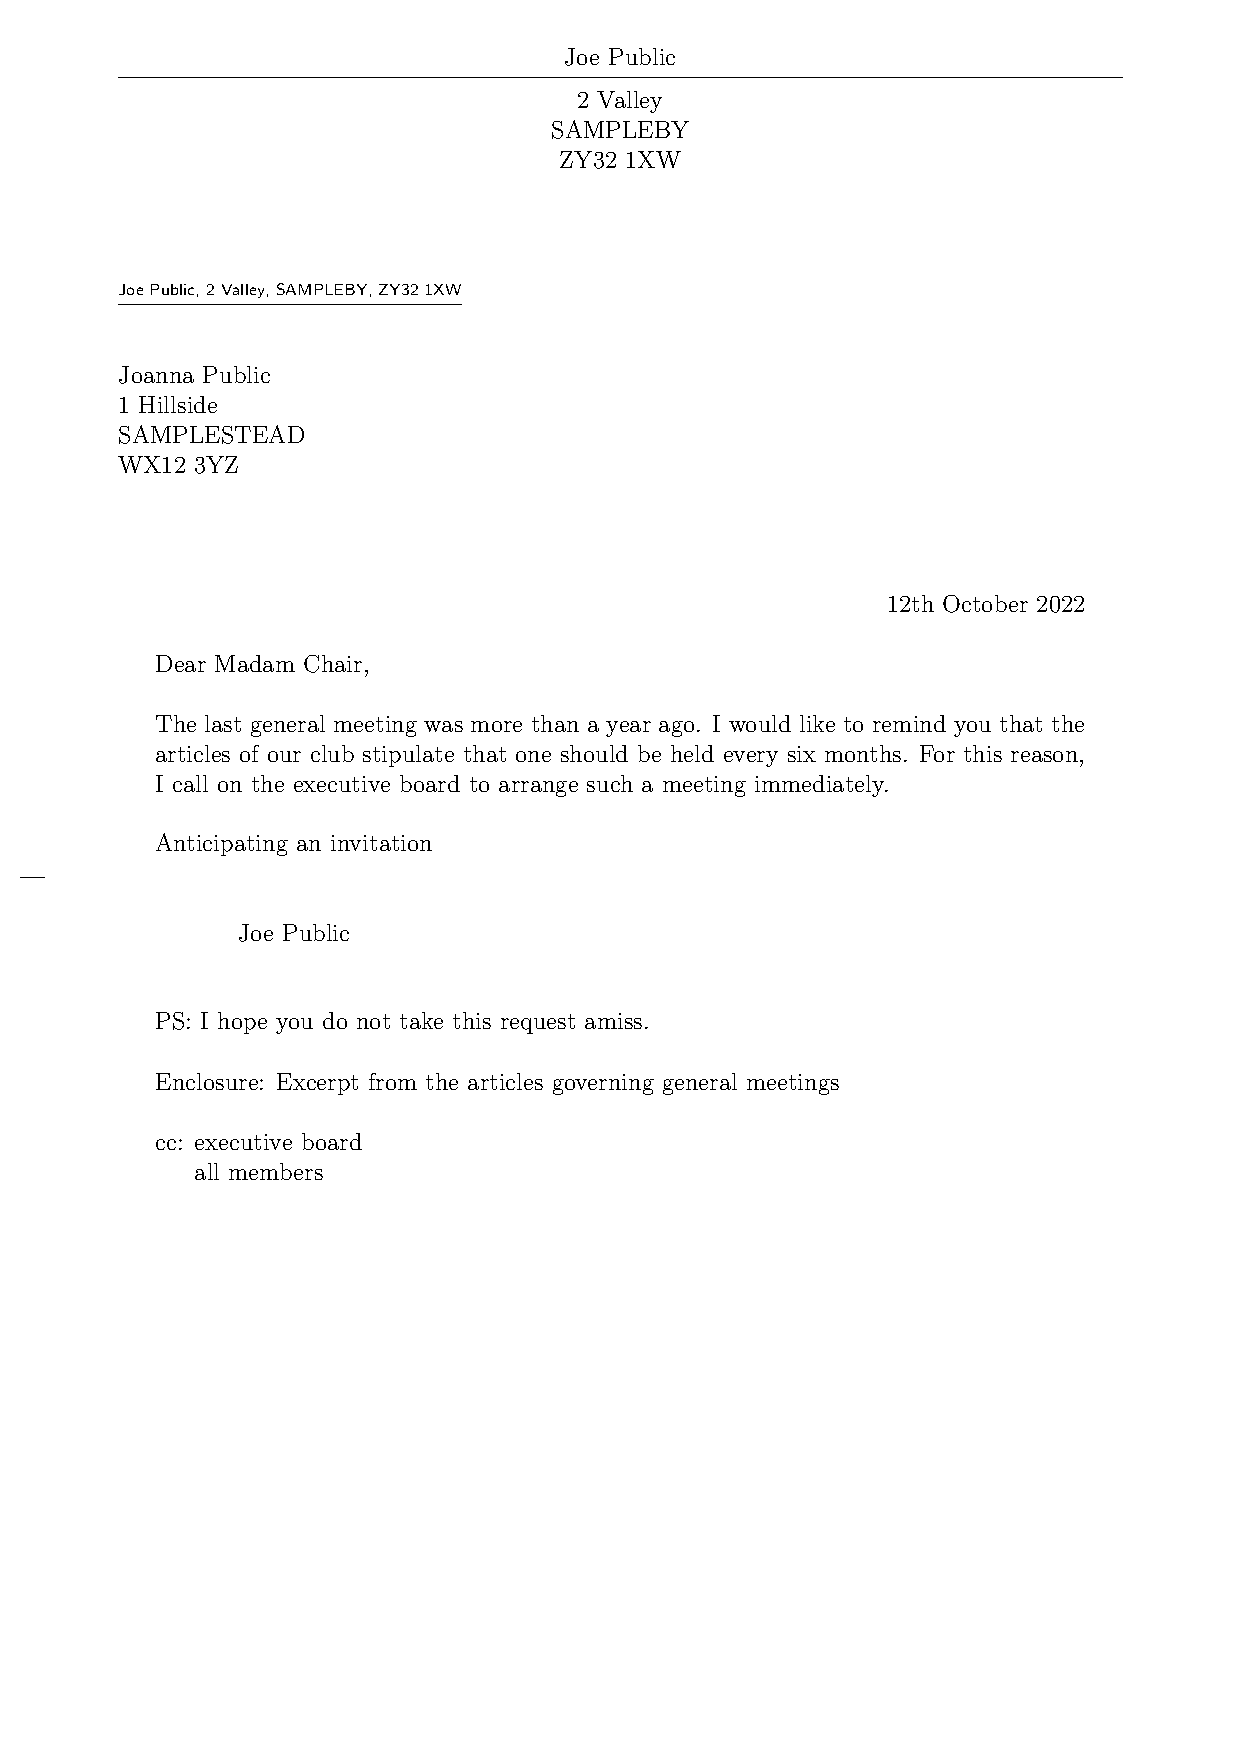
\includegraphics[width=.4\textwidth]{letter-example-10-en}}\quad
    \frame{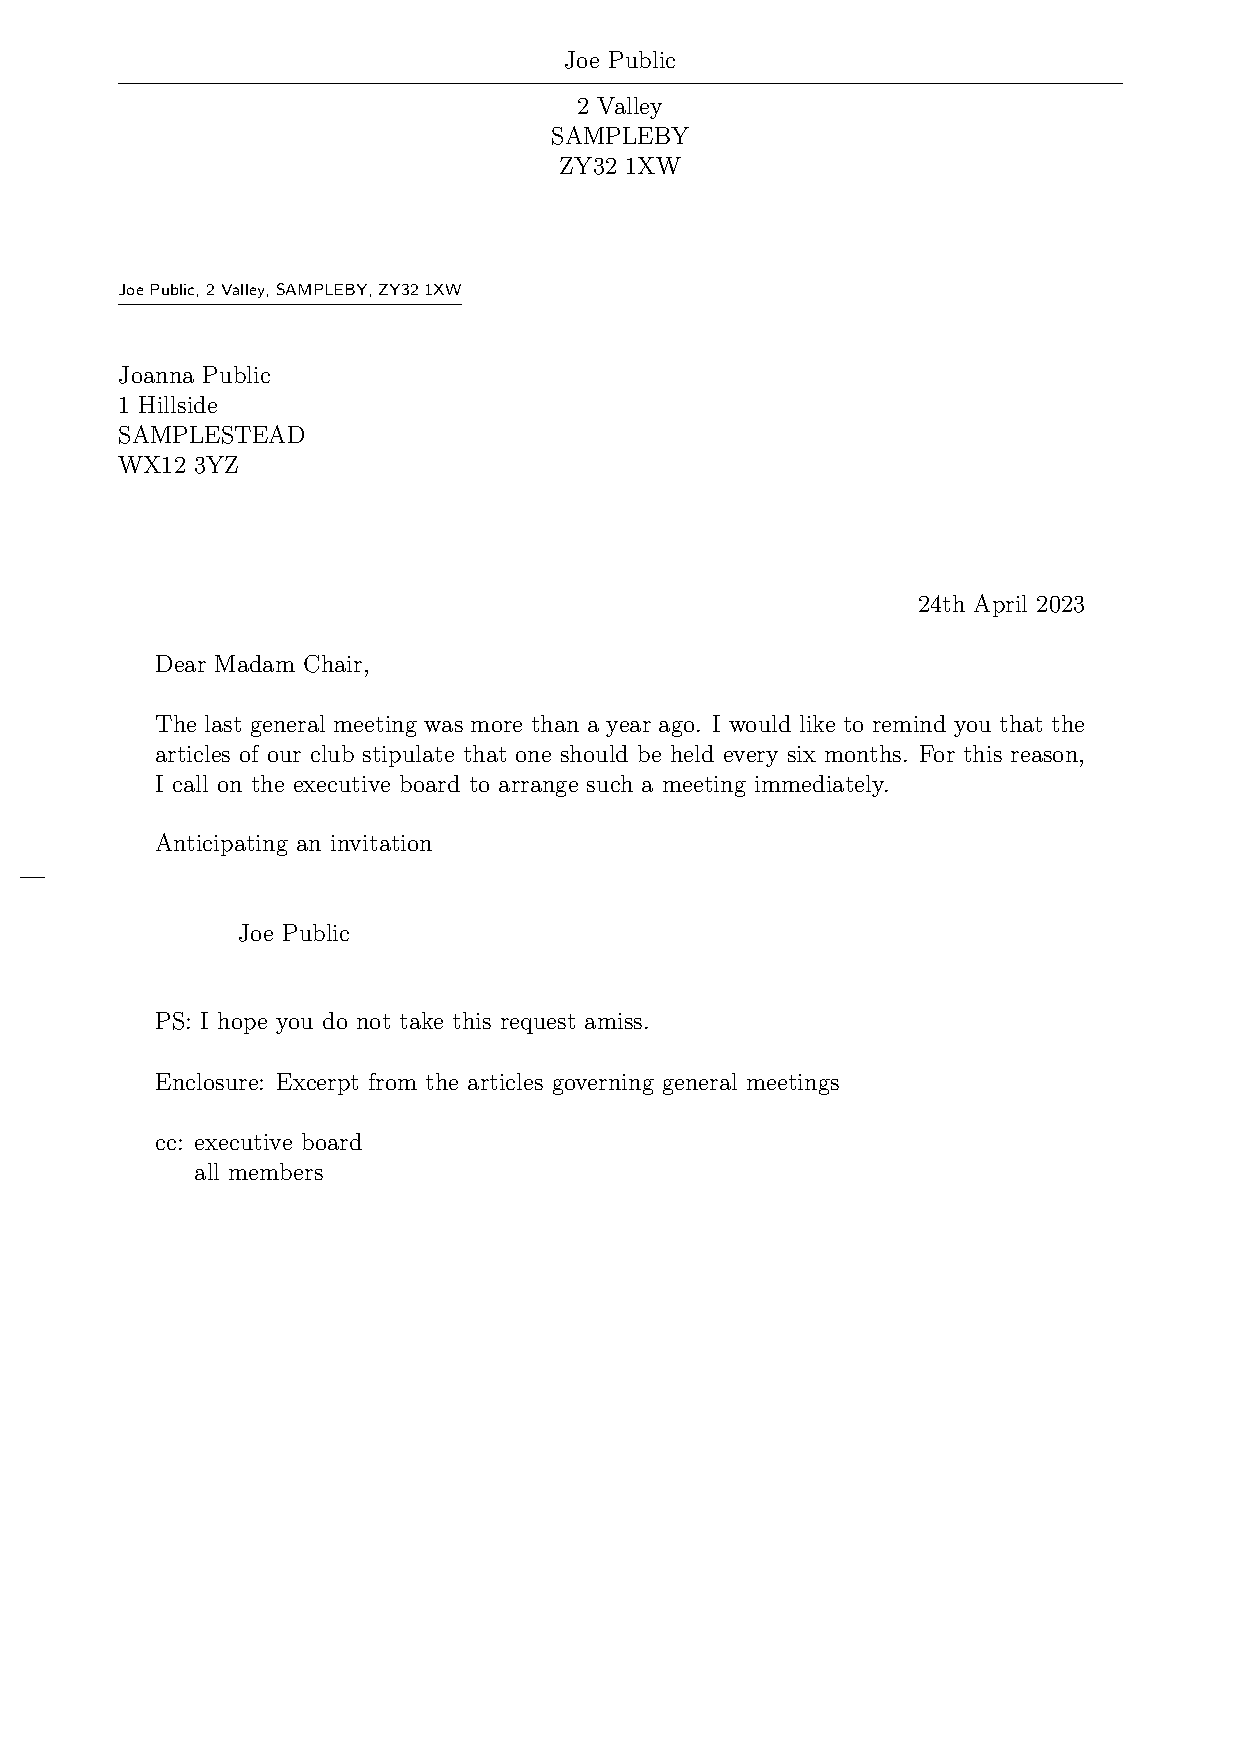
\includegraphics[width=.4\textwidth]{letter-example-11-en}}
    \caption[{Example: letter with sender, rule, recipient,
      opening, text, closing, signature, postscript, distribution list,
      enclosure, and hole-punch mark}]
    {result of a short letter with sender, rule, recipient,
      opening, text, closing, signature, postscript, distribution list,
      enclosure and hole-punch mark (the date is set by default):
      at left one the standard letterhead using
      \OptionValueRef{\LabelBase}{fromalign}{false}, at right one the extended letterhead
      using \OptionValueRef{\LabelBase}{fromalign}{center}}
    \label{fig:\LabelBase.letter-10-11}
  \end{figure}
\end{Example}

An\textnote{Attention!} important note concerns the sender's address: within
the sender's address, individual parts such as house number and street, city
and postal code, etc., are separated with a double backslash. This double
backslash is interpreted differently depending on how the sender's address is
used and therefore is not necessarily a line break. Paragraphs, vertical
spacing, and the like are usually not allowed within the sender's information.
You have to know \KOMAScript{} very well to put such things into the sender
information, if necessary. In addition, note that if you do so, you should
definitely set the variables for return address (see
\DescRef{\LabelBase.variable.backaddress},
\DescPageRef{\LabelBase.variable.backaddress}) and signature (see
\DescRef{\LabelBase.variable.signature},
\DescPageRef{\LabelBase.variable.signature}) yourself.%
%
\EndIndexGroup


\begin{Declaration}
  \PLength{fromrulethickness}%
  \PLength{fromrulewidth}
\end{Declaration}
As mentioned in the explanation of the
\DescRef{\LabelBase.option.fromrule}\IndexOption{fromrule} option in
\autoref{sec:\LabelBase.firstpage}, \DescPageRef{\LabelBase.option.fromrule}, you
can put a horizontal rule within or below the sender's address in the
predefined letterheads. If\textnote{Attention!} the \PLength{fromrulewidth}
pseudo-length has a value of 0\Unit{pt}, which is the default in the
predefined \File{lco} files, the length of this rule is calculated
automatically taking into account, for example, letterhead width or an
optional logo. You can adjust rule length manually in your own \File{lco}
files by setting this pseudo-length to positive values using
\Macro{setplength} (see \DescPageRef{\LabelBase.cmd.setplength}). The
default thickness of the line\ChangedAt{v2.97c}{\Class{scrlttr2}},
\PLength{fromrulethickness}, is 0.4\Unit{pt}.%
\EndIndexGroup


\begin{Declaration}
  \OptionVName{symbolicnames}{value}%
  \OptionVName{fromphone}{simple switch}%
  \OptionVName{frommobilephone}{simple switch}%
  \OptionVName{fromfax}{simple switch}%
  \OptionVName{fromemail}{simple switch}%
  \OptionVName{fromurl}{simple switch}%
  \Variable{fromphone}%
  \Variable{frommobilephone}%
  \Variable{fromfax}%
  \Variable{fromemail}%
  \Variable{fromurl}%
  \Variable{phoneseparator}%
  \Variable{mobilephoneseparator}%
  \Variable{faxseparator}%
  \Variable{emailseparator}%
  \Variable{urlseparator}%
\end{Declaration}
\BeginIndex{}{letterhead}%
\BeginIndex{}{letter>header}%
You can use the five options \Option{fromphone},
\Option{frommobilephone}\ChangedAt{v3.12}{\Class{scrlttr2}}, \Option{fromfax},
\Option{fromemail}, and \Option{fromurl} to specify whether to include the
phone number\Index{telephone}\Index{phone},
mobile\ChangedAt{v3.12}{\Class{scrlttr2}} phone number\Index{mobile
  phone}\Index{cell phone}\Index{cellphone}, fax number\Index{fax}, e-mail
address\Index{e-mail}, or URL should be as part of the sender's
information. You can assign any standard value for simple switches from
\autoref{tab:truefalseswitch}, \autopageref{tab:truefalseswitch} to these
options. The default for all of them is \PValue{false}. The \PName{contents}
themselves are determined by the variables of the same name. You can find the
defaults for the \PName{description} or title of each variable in
\autoref{tab:\LabelBase.fromTerm}. You can find the separators that will be
inserted between the \PName{description} and the \PName{content} in
\autoref{tab:\LabelBase.fromSeparator}.

You can\ChangedAt{v3.12}{\Class{scrlttr2}}\important{\Option{symbolicnames}}
change the defaults for describing the variables all at once with the
\Option{symbolicnames} option. This option understands the values for simple
switches found in \autoref{tab:truefalseswitch},
\autopageref{tab:truefalseswitch}.
Activating\ChangedAt{v3.27}{\Class{scrlttr2}\and \Package{scrletter}} the
option corresponds to \PName{value} \PValue{marvosym} and replaces the
descriptions from the language-dependent labels of
\DescRef{scrlttr2-experts.cmd.emailname},
\DescRef{scrlttr2-experts.cmd.faxname},
\DescRef{scrlttr2-experts.cmd.mobilephonename}, and
\DescRef{scrlttr2-experts.cmd.phonename} with symbols from the
\Package{marvosym}\IndexPackage{marvosym} package. At the same time, the colon
is omitted when defining the separators. In this case, both the description
and the content of the URL separator will be empty. With
\OptionValue{symbolicnames}{fontawesome} or
\OptionValue{symbolicnames}{awesome}, symbols of package
\Package{fontawesome}\IndexPackage{fontawesome} are used. In this case there
is also a symbol for the URL. Note\textnote{Attention!} that you may need to
load the \Package{marvosym} or \Package{fontawesome} package in your document
preamble if you activate the option for the corresponding package for the
first time after \Macro{begin}\PParameter{document}.

\begin{table}
  \centering
  \caption[{Default descriptions of the letterhead variables}]{Default
    descriptions of the letterhead variables (you can find the description and
    contents of the separator variables in
    \autoref{tab:\LabelBase.fromSeparator}}
  \begin{desctabular}[1.8em]
    \ventry{fromemail}{\DescRef{\LabelBase.cmd.usekomavar*}\PParameter{emailseparator}%
      \DescRef{\LabelBase.cmd.usekomavar}\PParameter{emailseparator}}%
    \ventry{fromfax}{\DescRef{\LabelBase.cmd.usekomavar*}\PParameter{faxseparator}%
      \DescRef{\LabelBase.cmd.usekomavar}\PParameter{faxseparator}}%
    \ventry{frommobilephone}{%
      \ChangedAt{v3.12}{\Class{scrlttr2}}%
      \DescRef{\LabelBase.cmd.usekomavar*}\PParameter{mobilephoneseparator}%
      \DescRef{\LabelBase.cmd.usekomavar}\PParameter{mobilephoneseparator}}%
    \ventry{fromname}{\DescRef{scrlttr2-experts.cmd.headfromname}}%
    \ventry{fromphone}{\DescRef{\LabelBase.cmd.usekomavar*}\PParameter{phoneseparator}%
      \DescRef{\LabelBase.cmd.usekomavar}\PParameter{phoneseparator}}%
    \ventry{fromurl}{\DescRef{\LabelBase.cmd.usekomavar*}\PParameter{urlseparator}%
      \DescRef{\LabelBase.cmd.usekomavar}\PParameter{urlseparator}}%
  \end{desctabular}
  \label{tab:\LabelBase.fromTerm}
\end{table}

\begin{table}[tp]
  \centering
%  \KOMAoptions{captions=topbeside}%
%  \setcapindent{0pt}%
  \caption{Default descriptions and contents of the letterhead
    separators without the \Option{symbolicnames} option}
%    [l]
  \begin{tabular}[t]{lll}
    \toprule
    variable name             & description       & content \\
    \midrule
    \Variable{emailseparator} & \DescRef{scrlttr2-experts.cmd.emailname} & \texttt{:\~} \\
    \Variable{faxseparator}   & \DescRef{scrlttr2-experts.cmd.faxname}   & \texttt{:\~} \\
    \Variable{mobilephoneseparator} & \DescRef{scrlttr2-experts.cmd.mobilephonename} & \Macro{usekomavaer}\PParameter{phoneseparator} \\
    \Variable{phoneseparator} & \DescRef{scrlttr2-experts.cmd.phonename} & \texttt{:\~} \\
    \Variable{urlseparator}   & \DescRef{scrlttr2-experts.cmd.wwwname}   & \texttt{:\~} \\
    \bottomrule
  \end{tabular}
%  \end{captionbeside}
  \label{tab:\LabelBase.fromSeparator}
\end{table}

\begin{Example}
  Mr Public from our sample letter has a telephone and an e-mail address. He
  also wants to show these in the letterhead. At the same time, the separation
  rule should now be placed after the letterhead. So he uses the appropriate
  options and also sets the required variables:%
  \lstinputcode[xleftmargin=1em]{letter-example-12-en.tex}%
  The results on the left side of \autoref{fig:\LabelBase.letter-12-13},
  however, are confounding: the options are ignored. That's because the
  additional variables and options are only used in the extended letterhead.
  So the \DescRef{\LabelBase.option.fromalign} option must be used, as it is
  in the right side of
  \autoref{fig:\LabelBase.letter-12-13}.
  \begin{figure}
    \centering
    \frame{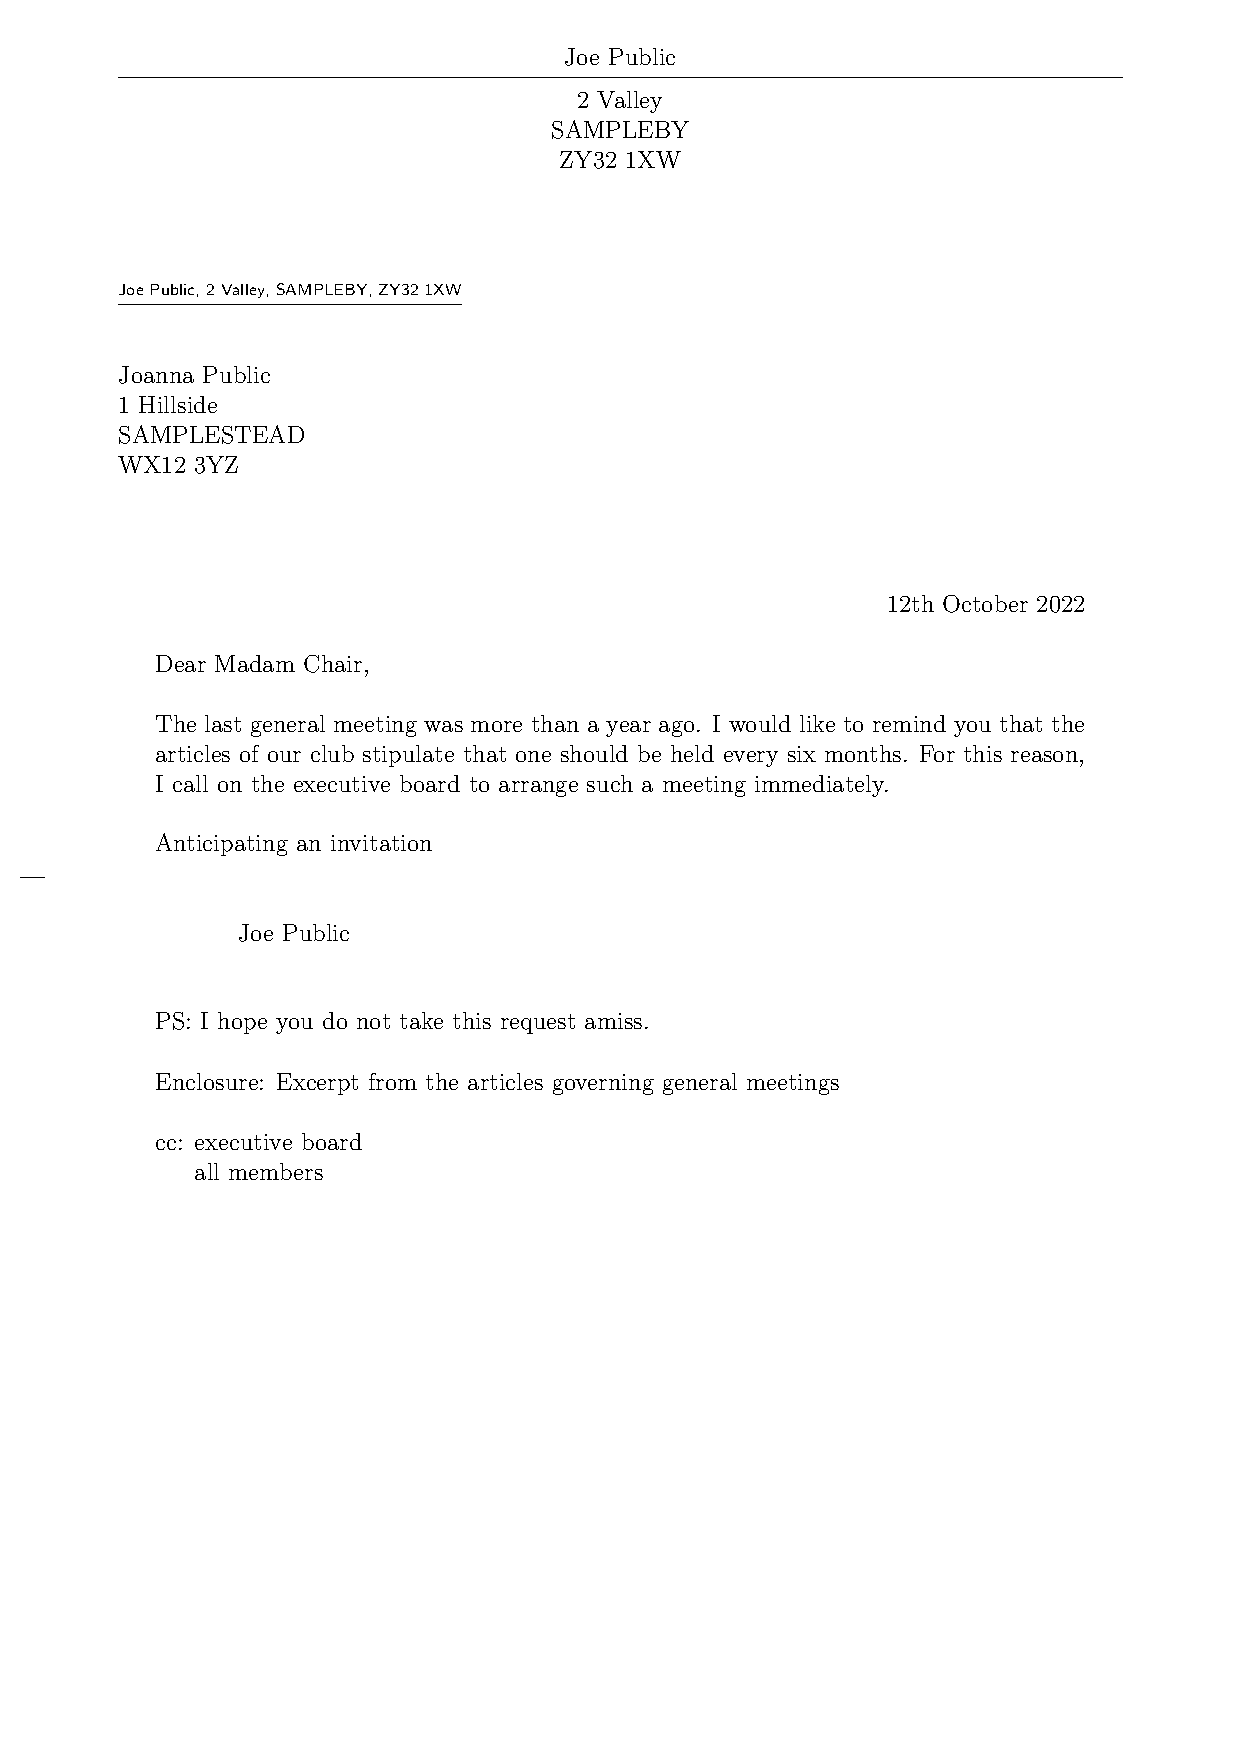
\includegraphics[width=.4\textwidth]{letter-example-12-en}}\quad
    \frame{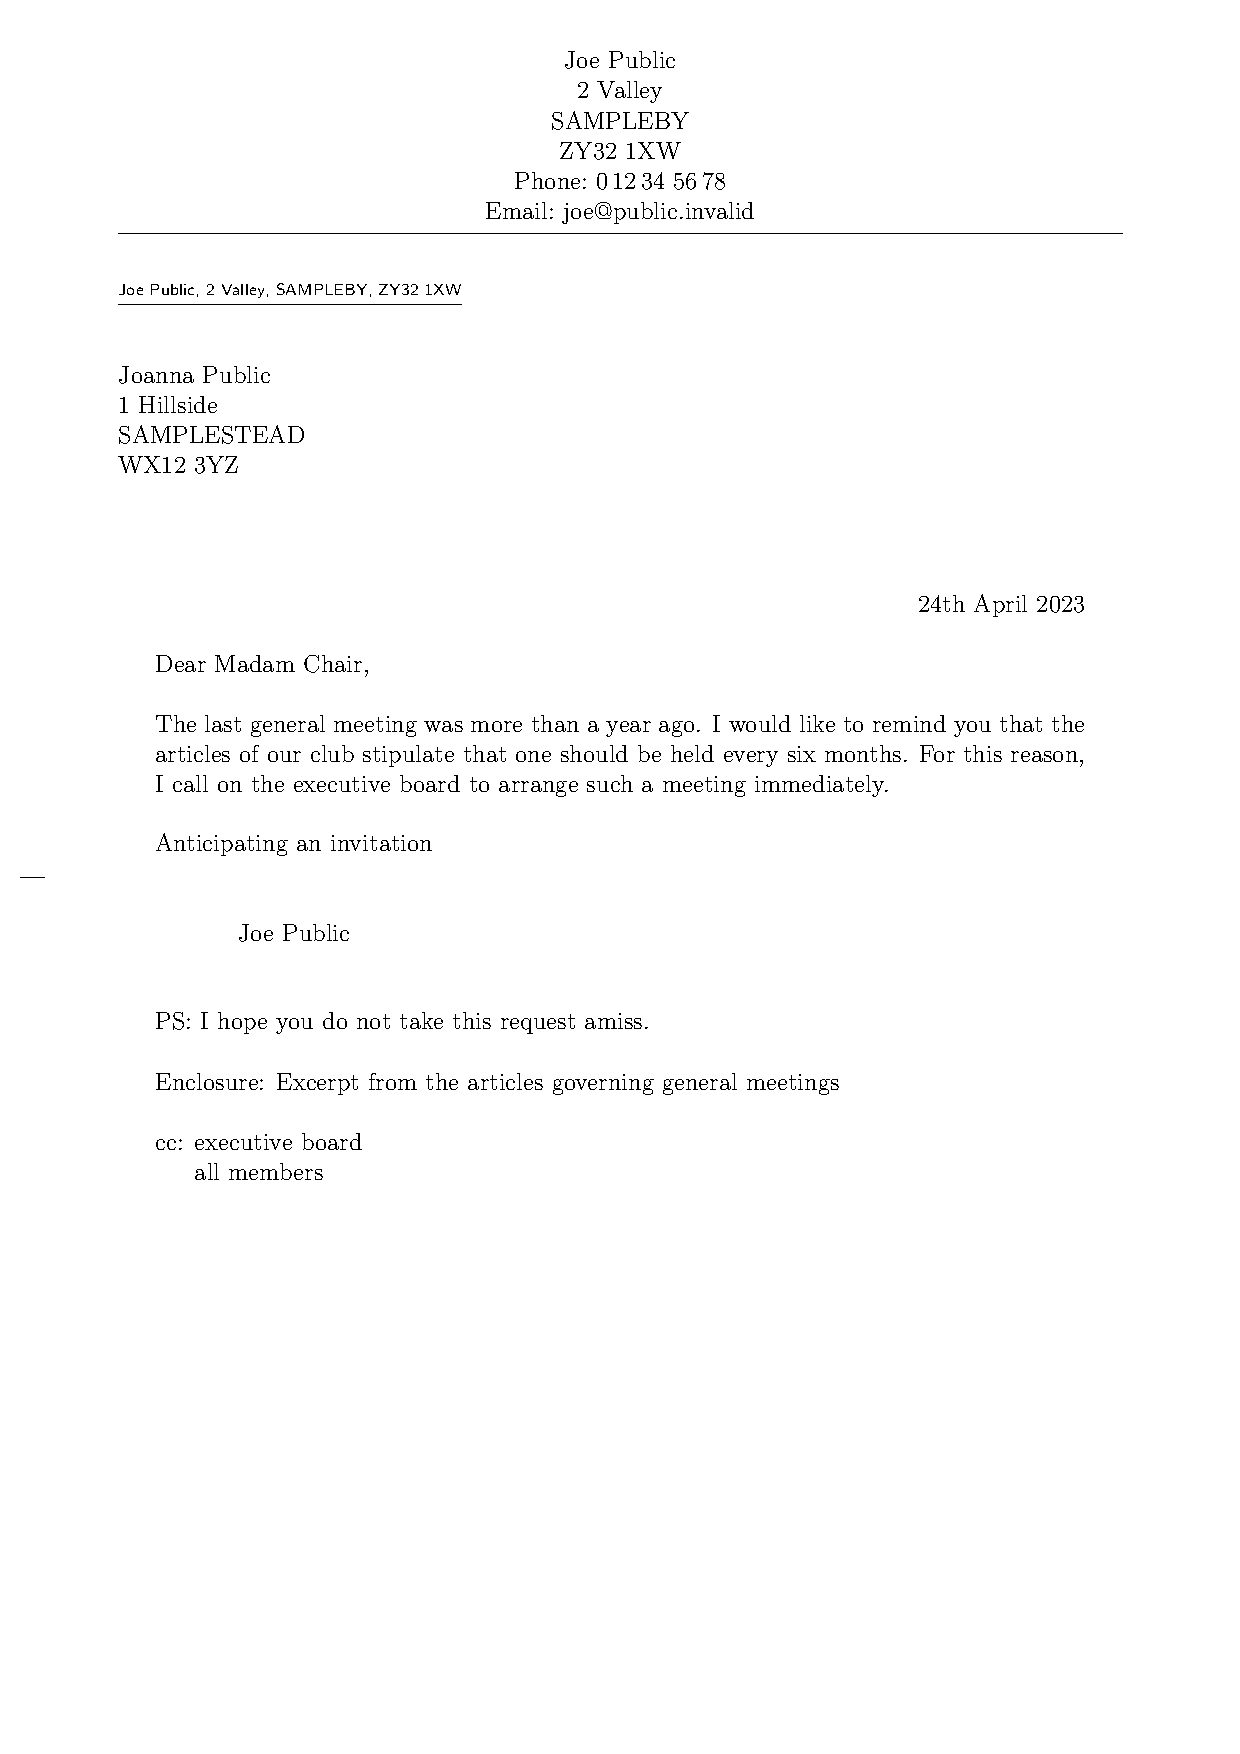
\includegraphics[width=.4\textwidth]{letter-example-13-en}}
    \caption[{Example: letter with extra sender information, rule,
      recipient, opening, text, closing, signature, postscript, distribution
      list, enclosure, and hole-punch mark; standard vs. extended letterhead}]
    {result of a short letter with sender, rule, recipient, opening, text,
      closing, signature, postscript, distribution list, enclosure and
      hole-punch mark (the date is set by default): the left one uses the
      standard letterhead with
      \OptionValueRef{\LabelBase}{fromalign}{false}; the right one uses the
      extended letterhead with \OptionValueRef{\LabelBase}{fromalign}{center}}
    \label{fig:\LabelBase.letter-12-13}
  \end{figure}
  \lstinputcode[xleftmargin=1em]{letter-example-13-en.tex}

  You can compare two other alternatives with left-aligned sender information using
  \OptionValueRef{\LabelBase}{fromalign}{left} and right-aligned sender information
  using \OptionValueRef{\LabelBase}{fromalign}{right} in
  \autoref{fig:\LabelBase.letter-14-15}.
  \begin{figure}
    \centering
    \frame{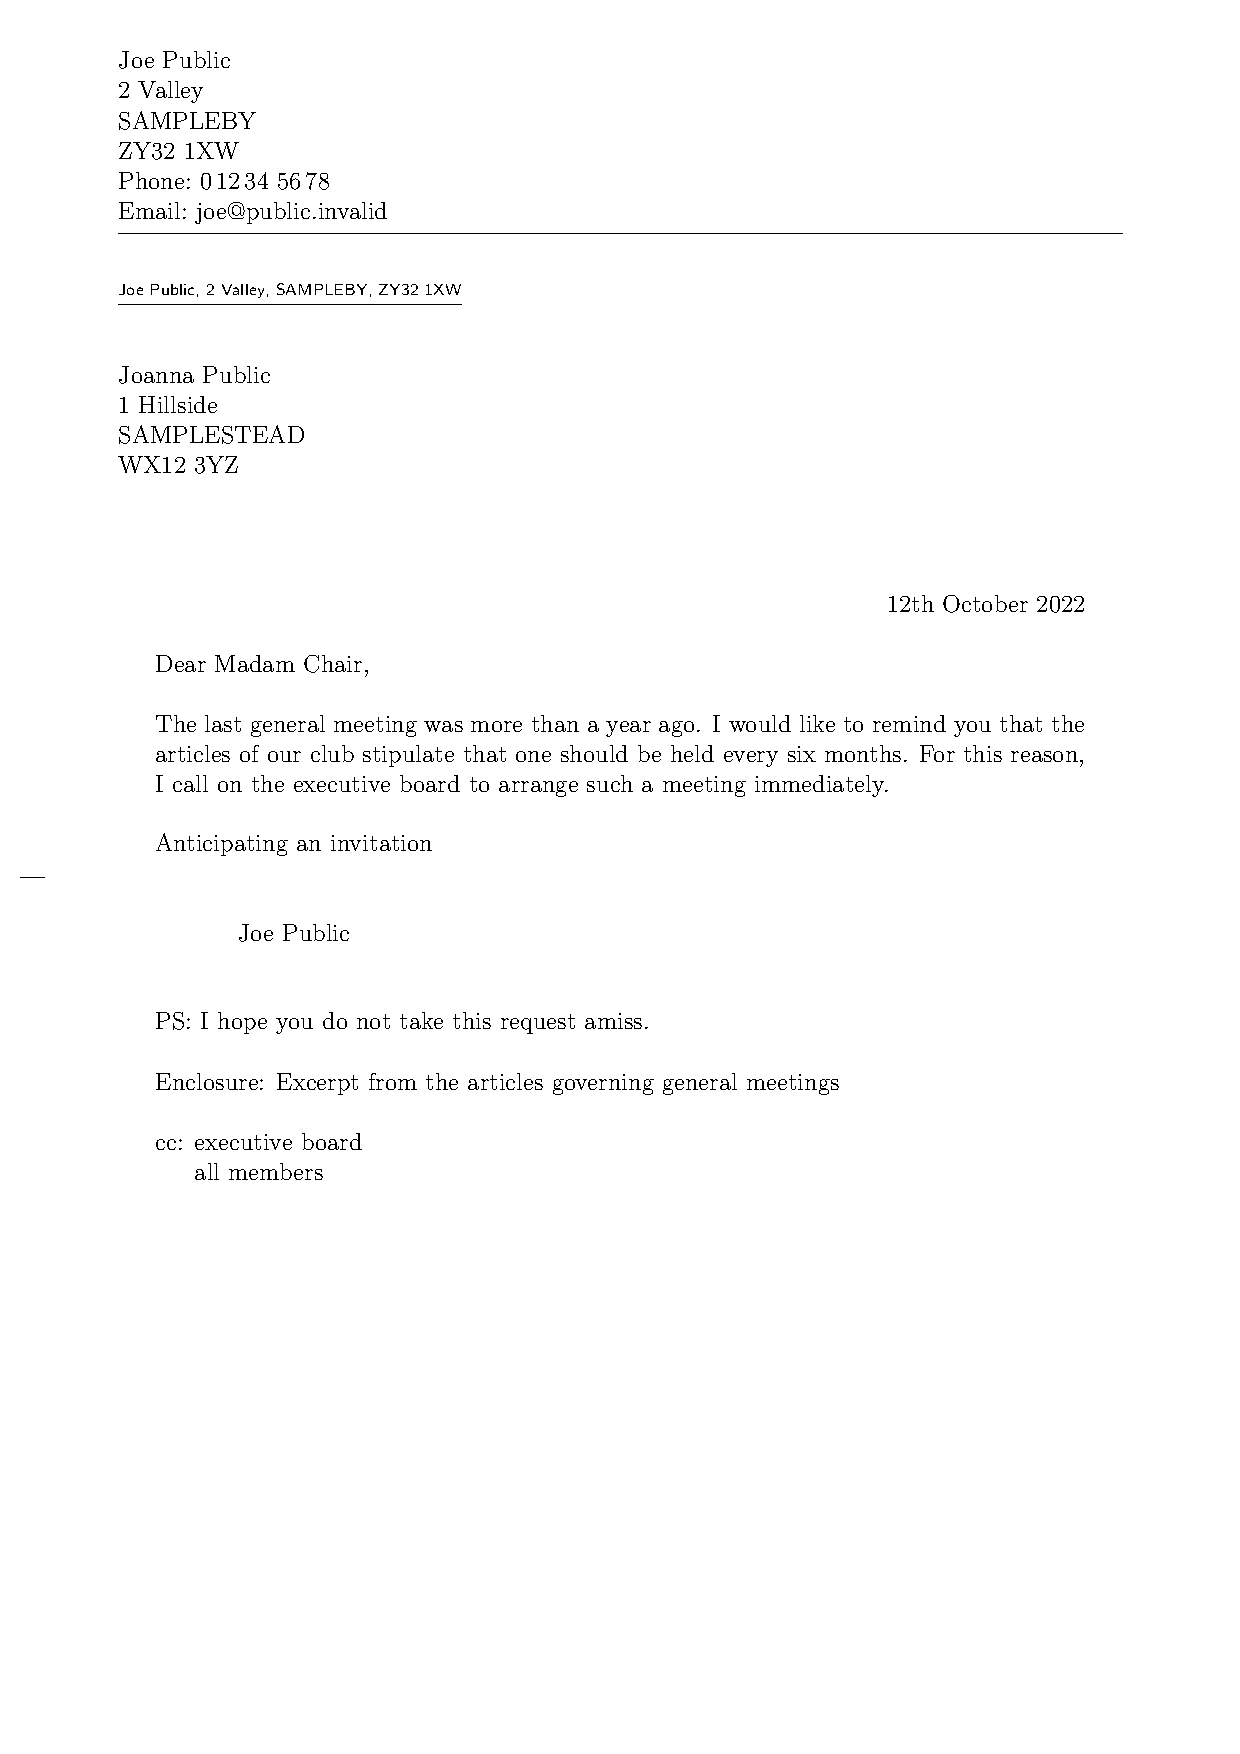
\includegraphics[width=.4\textwidth]{letter-example-14-en}}\quad
    \frame{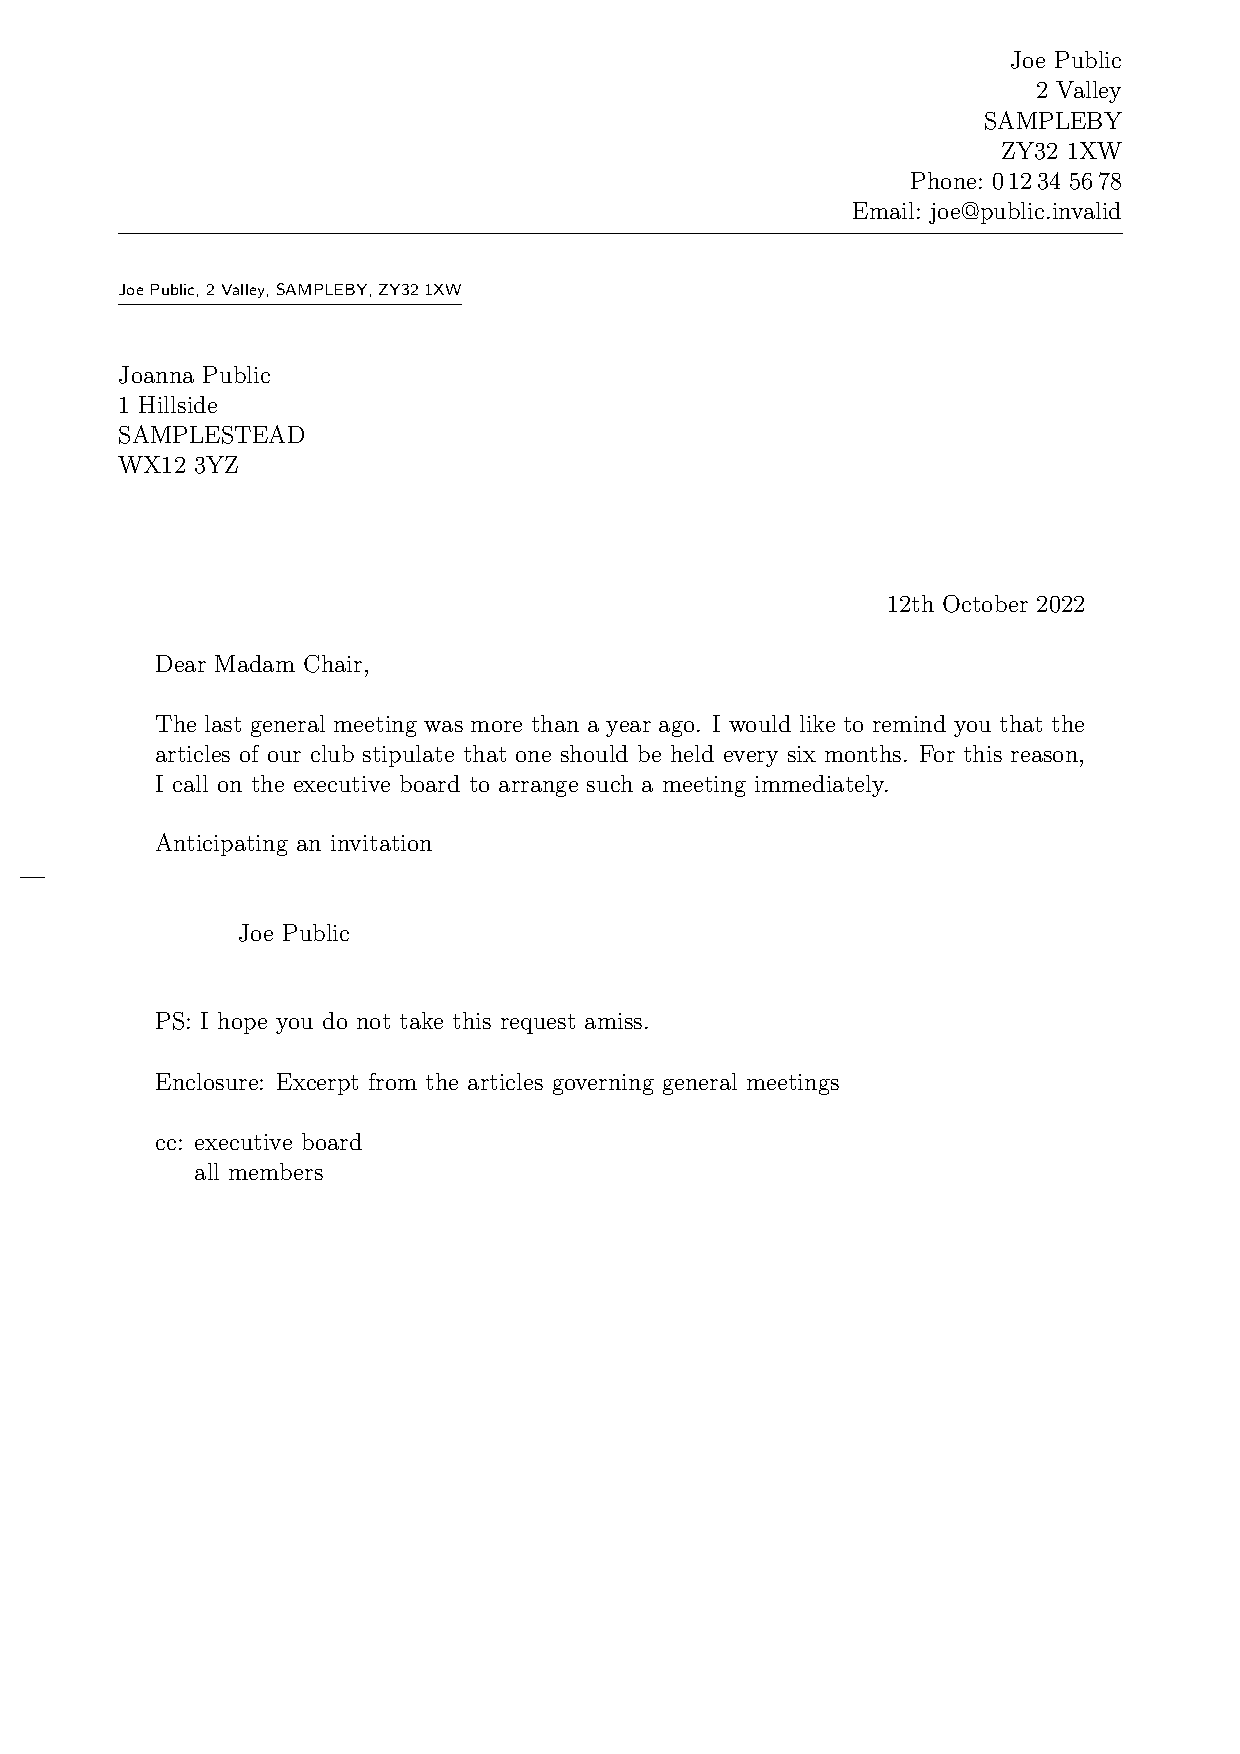
\includegraphics[width=.4\textwidth]{letter-example-15-en}}
    \caption[{Example: letter with extra sender information, rule,
      recipient, opening, text, closing, signature, postscript, distribution
      list, enclosure, and hole-punch mark; left- vs. right-aligned
      letterhead}]
    {result of a short letter with extra sender information, rule,
      recipient, opening, text, closing, signature, postscript, distribution
      list, enclosure and hole-punch mark (the date is set by default):
      the left one uses a left-aligned letterhead with
      \OptionValueRef{\LabelBase}{fromalign}{left}; the right one uses a
      right-aligned letterhead using
      \OptionValueRef{\LabelBase}{fromalign}{right}}
    \label{fig:\LabelBase.letter-14-15}
  \end{figure}
\end{Example}
%
\EndIndexGroup


\begin{Declaration}
  \OptionVName{fromlogo}{simple switch}%
  \Variable{fromlogo}%
\end{Declaration}
\BeginIndex{}{letterhead}%
\BeginIndex{}{letter>head}%
You can use the \Option{fromlogo} to configure whether to put a
logo\Index{Logo} in the letterhead. You can use any of the default values from
\autoref{tab:truefalseswitch}, \autopageref{tab:truefalseswitch} for the
\PName{simple switch}. The default is \PValue{false}, which means no logo. The
logo itself is defined by the \PName{content} of the \Variable{fromlogo}
variable. The \PName{description} of the logo is empty by default and
\KOMAScript{} does not use it in the default letterhead pages.%
\begin{Example}
  Mr Public finds it particularly stylish when he provides his letterhead with
  a logo. He has saved his logo as a graphics file, which he would like to
  load using \Macro{includegraphics}. To do this, he loads the
  \Package{graphics}\IndexPackage{graphics} package (see
  \cite{package:graphics}).%
  \lstinputcode[xleftmargin=1em]{letter-example-16-en.tex}%
  You can see the result in the top left of
  \autoref{fig:\LabelBase.letter-16-18}. The other two images in this figure
  show the results with right-aligned and centred sender information.
  \begin{figure}
    \setcapindent{0pt}%
    {\hfill
      \frame{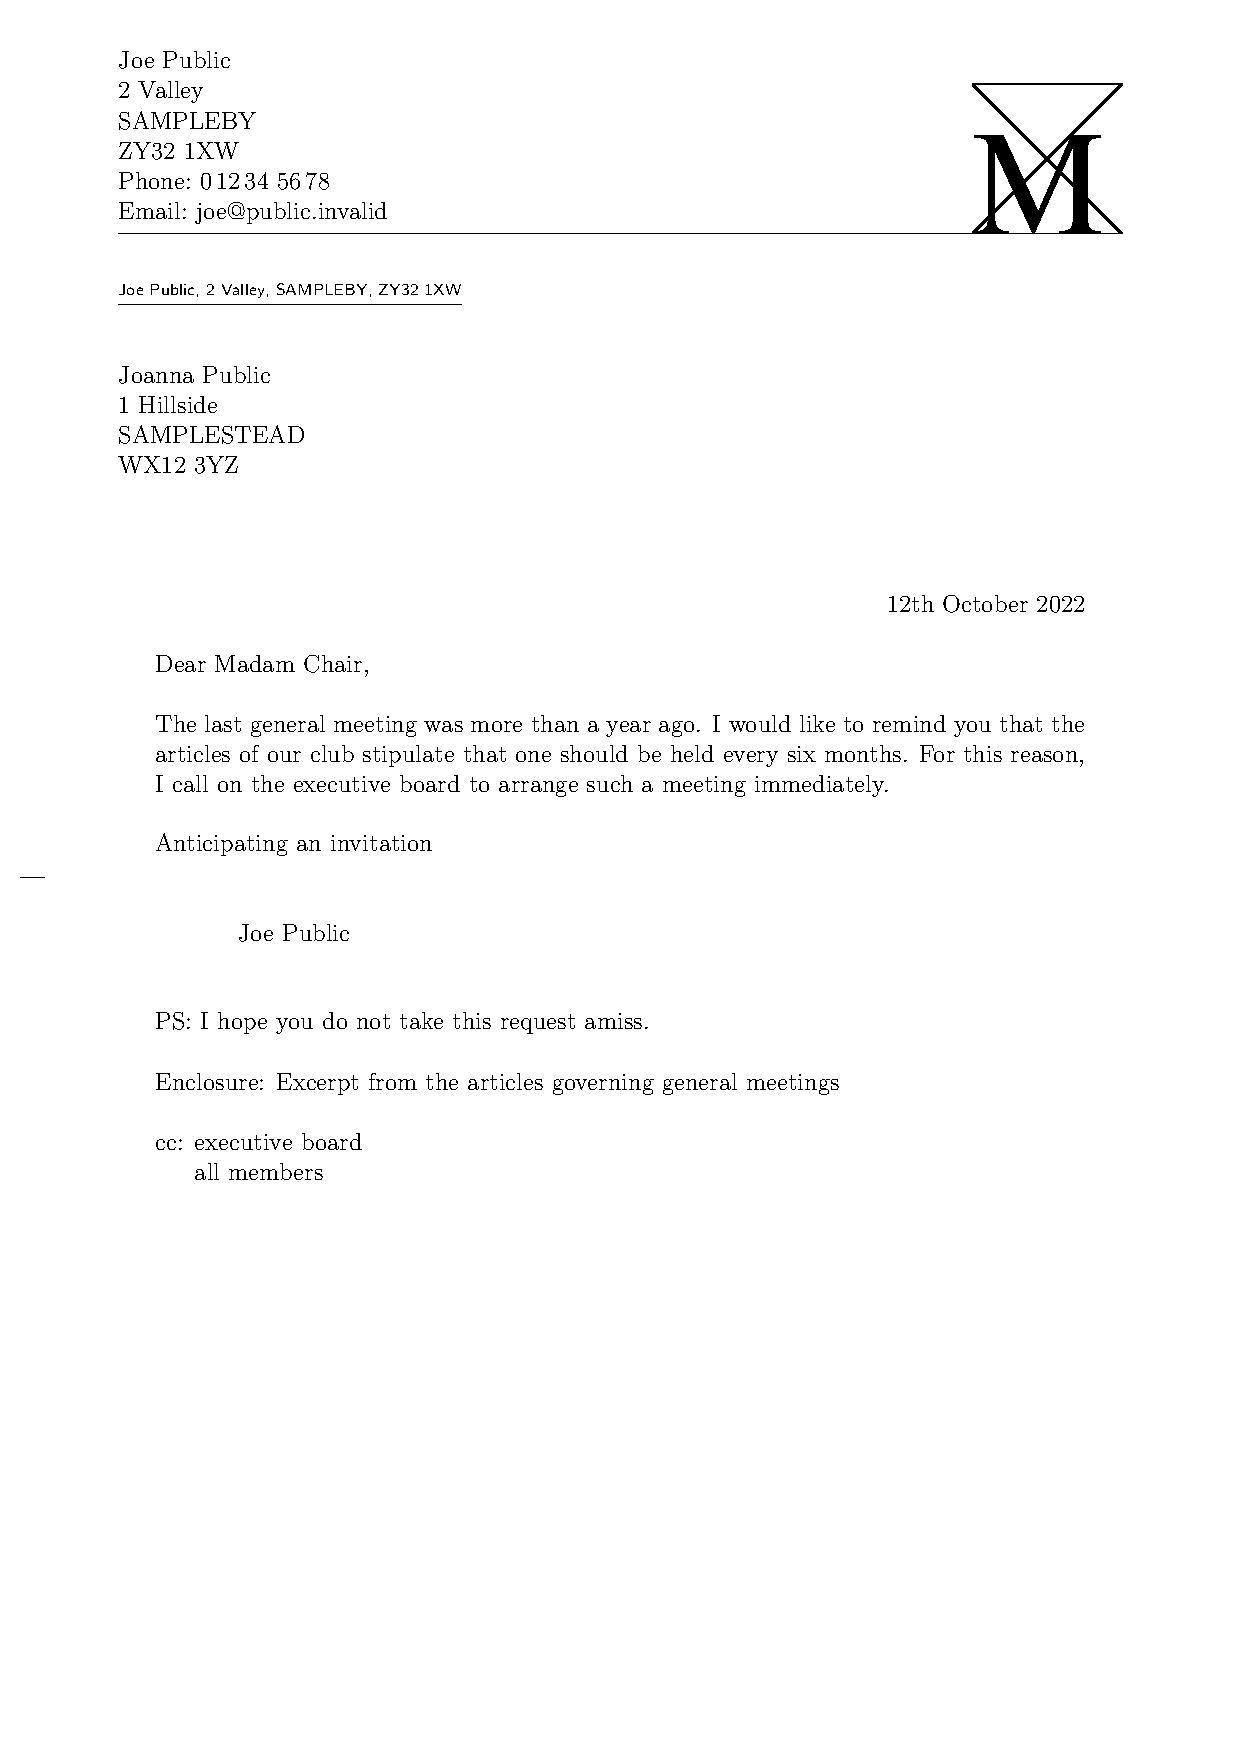
\includegraphics[width=.4\textwidth]{letter-example-16-en}}\quad
      \frame{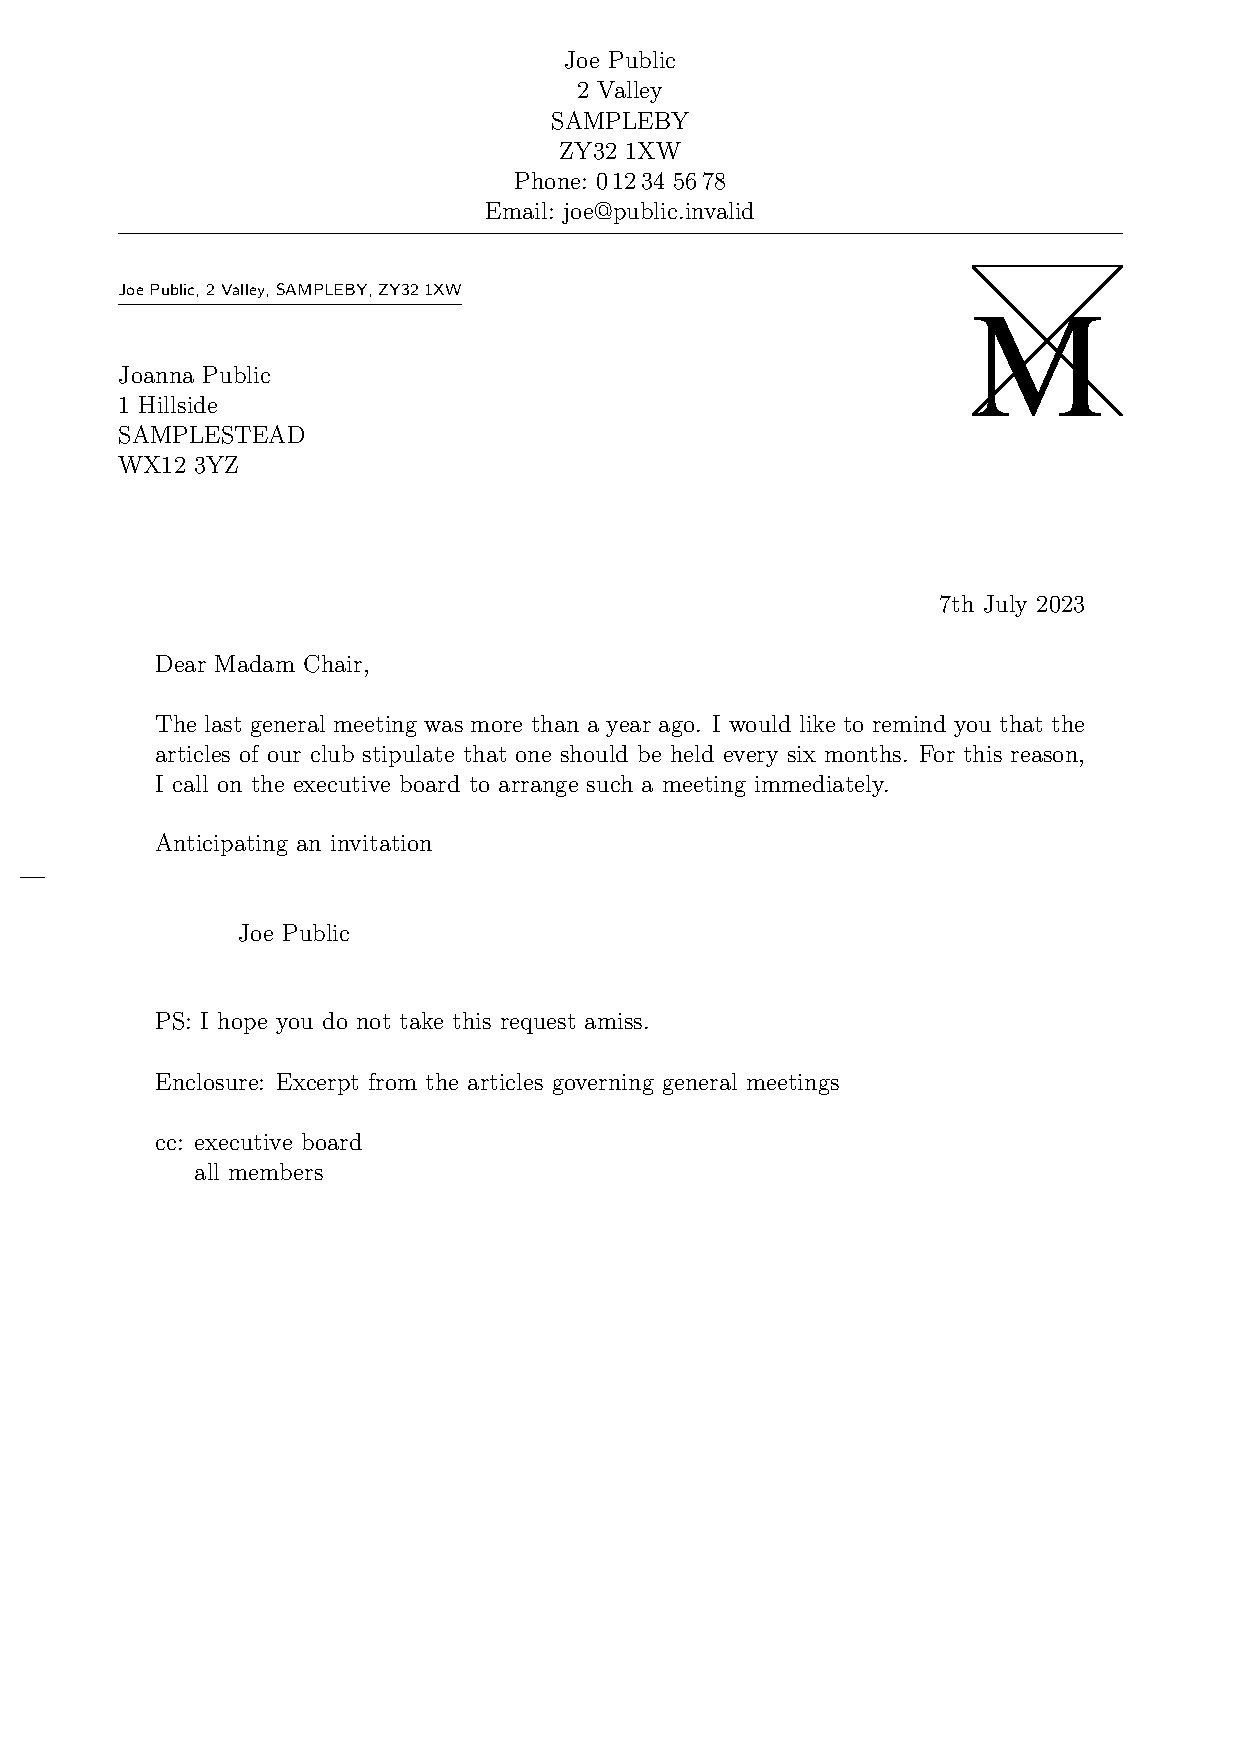
\includegraphics[width=.4\textwidth]{letter-example-17-en}}\par\bigskip}
    \begin{captionbeside}[{Example: letter with extra sender information,
        logo, rule, recipient, opening, text, closing, signature, postscript,
        distribution list, enclosure, and hole-punch mark; left-aligned vs.
        right-aligned vs. centred sender information}]
      {result of a short letter with extra sender information, logo, rule,
        recipient, opening, text, closing, signature, postscript, distribution
        list, enclosure and hole-punch mark (the date is set by default):
        at top left the sender is left-aligned, at top right the sender is
        centred, and at bottom right the sender is right-aligned
        sender}[l]
      \frame{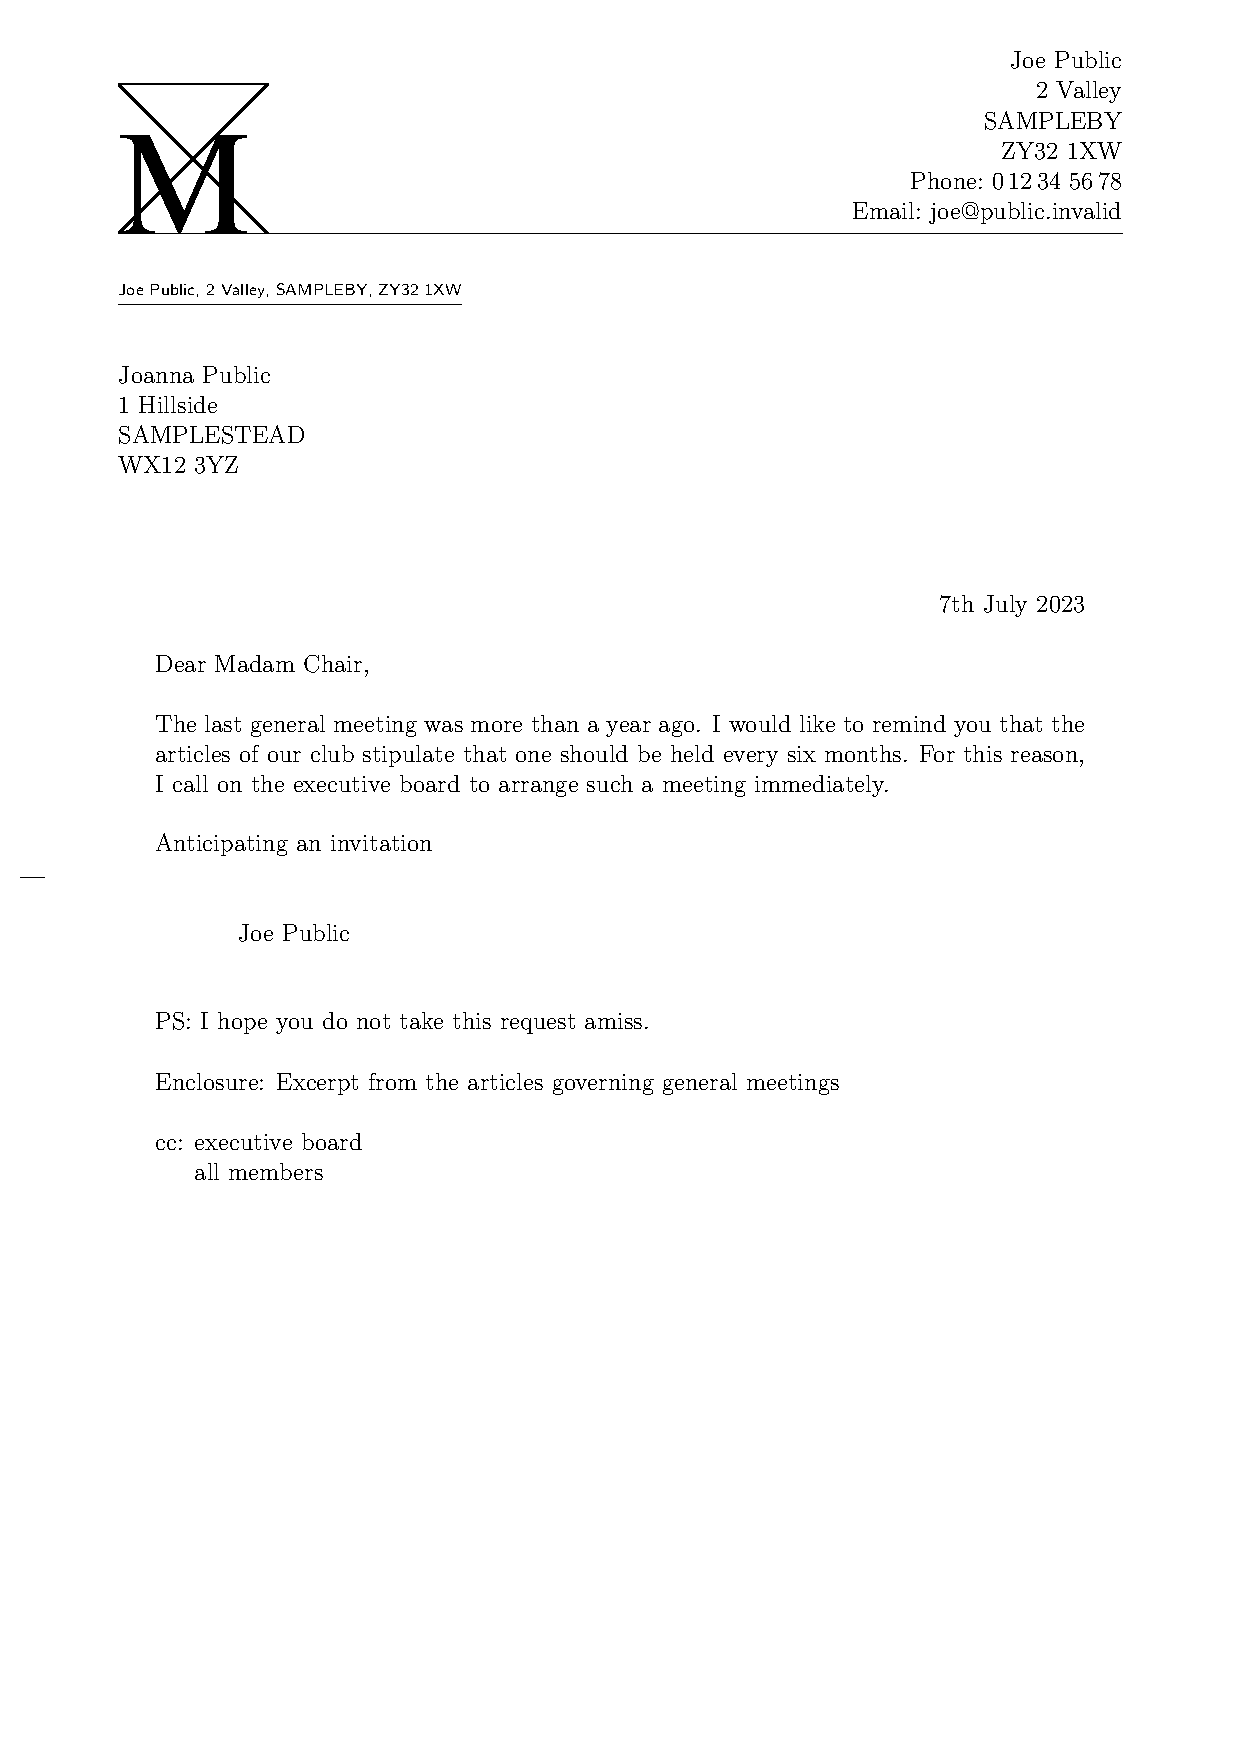
\includegraphics[width=.4\textwidth]{letter-example-18-en}}\quad
    \end{captionbeside}
  \label{fig:\LabelBase.letter-16-18}
  \end{figure}
\end{Example}%
%
\EndIndexGroup


\begin{Declaration}
  \Variable{firsthead}%
\end{Declaration}
In many cases, the capabilities that \Class{scrlttr2} offers with the
foregoing options and variables will be sufficient to design a letterhead. In
some cases, however, you may want even more flexibility. In those situations,
you will have to do without the possibilities offered by the predefined
letterhead, which you can select via the options described above. Instead, you
must create your own letterhead from scratch. To do so, you must specify the
desired structure as the \PName{contents} of the \Variable{firsthead}
variable. For example, you can set several boxes side by side or one beneath
the other using the \Macro{parbox} command (see \cite{latex:usrguide}).
Experienced users should thus be able to create their own a letterheads. Of
course you can and should use other variables with
\DescRef{\LabelBase.cmd.usekomavar}. \KOMAScript{} does not use the
\PName{description} of variable \Variable{firsthead}. \iffree{}{You can find
  a detailed example of a letterhead definition in
  \autoref{cha:modernletters}.}%
\EndIndexGroup
%
\EndIndexGroup


\subsection{Addressee}
\seclabel{addressee}%
\BeginIndexGroup
\BeginIndex{}{addressee}
\index{recipient|seealso{addressee}}

The term \emph{addressee} normally refers only to the recipient's name and
address, which are output in an address field. Additional information,
however, can be placed within this address field, including the delivery
method, for example registered mail or special delivery. For window envelopes,
the return address also counts as part of the address field, as it will be
displayed in the address window. The address field directly follows the
letterhead.

\begin{Declaration}
  \OptionVName{addrfield}{format}%
  \OptionVName{backaddress}{value}%
  \OptionVName{priority}{priority}%
  \Variable{toname}%
  \Variable{toaddress}%
  \Variable{backaddress}%
  \Variable{backaddressseparator}%
  \Variable{specialmail}%
  \Variable{fromzipcode}%
  \Variable{zipcodeseparator}%
  \Variable{place}%
  \Variable{PPcode}%
  \Variable{PPdatamatrix}%
  \Variable{addresseeimage}%
\end{Declaration}%
\BeginIndex{}{address}%
The \Option{addrfield} option determines whether or not to print an address
field. The default\textnote{default} is to include an address field. The
option recognizes the formats described in
\autoref{tab:\LabelBase.addrfield}\ChangedAt{v3.03}{\Class{scrlttr2}}. With
the values \PValue{true},
\PValue{topaligned}\ChangedAt{v3.17}{\Class{scrlttr2}\and
\Package{scrletter}}, \PValue{PP}, and \PValue{backgroundimage}, the name and
address of the recipient are determined by the mandatory argument of the
\DescRef{\LabelBase.env.letter} environment (see
\autoref{sec:\LabelBase.document}, \DescPageRef{\LabelBase.env.letter}). This
information is also copied into the variables \Variable{toname} and
\Variable{toaddress}.

\BeginIndexGroup
\BeginIndex{FontElement}{addressee}\LabelFontElement{addressee}%
\BeginIndex{FontElement}{toname}\LabelFontElement{toname}%
\BeginIndex{FontElement}{toaddress}\LabelFontElement{toaddress}%
You can change the default font styles\ChangedAt{v2.97c}{\Class{scrlttr2}}
with the \DescRef{\LabelBase.cmd.setkomafont} or
\DescRef{\LabelBase.cmd.addtokomafont} commands (see
\autoref{sec:\LabelBase.textmarkup},
\DescPageRef{\LabelBase.cmd.setkomafont}). There are three elements. First,
the \FontElement{addressee}\important{\FontElement{addressee}} element is
responsible for the overall style of the recipient's name and address. The
elements \FontElement{toname}\important{\FontElement{toname}} and
\FontElement{toaddress}\important{\FontElement{toaddress}} are responsible
only for the name and the address of the recipient, respectively. You can use
\FontElement{toname} and \FontElement{toaddress} to define modifications from
the basic \FontElement{addressee} configuration.%
\EndIndexGroup
%
\begin{table}
  \caption[{Available values for the \Option{addrfield} option with
    \Class{scrlttr2}}]{Available values for the \Option{addrfield} option to
    change the recipient format of \Class{scrlttr2}}%
    \label{tab:\LabelBase.addrfield}%
  \begin{desctabular}
    \entry{\PValue{backgroundimage}, \PValue{PPbackgroundimage},
      \PValue{PPBackgroundImage}, \PValue{PPBackGroundImage},
      \PValue{ppbackgroundimage}, \PValue{ppBackgroundImage},
      \PValue{ppBackGroundImage}}{%
      Prints an address with a background image stored in the
      \Variable{addresseimage} variable as the postpaid postmark, but without
      a return address or delivery type.}%
    \entry{\PValue{false}, \PValue{off}, \PValue{no}}{%
      Does not print an address.}%
    \entry{\PValue{image}, \PValue{Image}, \PValue{PPimage}, \PValue{PPImage},
      \PValue{ppimage}, \PValue{ppImage}}{%
      Prints an image stored in the \Variable{addresseeimage} variable as an
      address with a postpaid postmark. Recipient information, return address,
      and delivery type or priority are ignored.}%
    \entry{\PValue{PP}, \PValue{pp}, \PValue{PPexplicite},
      \PValue{PPExplicite}, \PValue{ppexplicite}, \PValue{ppExplicite}}{%
      Prints an address with a postage print impression (pospaid) header
      filled in with the variables \Variable{fromzipcode}, \Variable{place},
      and \Variable{PPcode}, and when applicable with a priority and a data
      array defined by \Variable{PPdatamatrix}, but without a return address
      or delivery type.}%
    \entry{\PValue{topaligned}, \PValue{alignedtop}%
      \ChangedAt{v3.17}{\Class{scrlttr2}\and \Package{scrletter}}}{%
      Prints an address including a return address and a delivery type
      or priority. The address is not centred vertically beneath the delivery
      type.}%
    \entry{\PValue{true}, \PValue{on}, \PValue{yes}}{%
      Prints an address field including a return address and delivery type
      or priority.}%
  \end{desctabular}
\end{table}%

The default \OptionValue{addrfield}{true} also prints an underlined return
address in the address field. The \Option{backaddress} option defines if and
in what form a return address will be printed for window envelopes. On the one
hand, this option\important{\OptionValue{backaddress}{false}} accepts the
standard values for simple switches listed in \autoref{tab:truefalseswitch},
\autopageref{tab:truefalseswitch}. These values do not change style of the
return address. On the other hand, when\ChangedAt{v2.96}{\Class{scrlttr2}} the
return address is enabled, you can select its format at the same time. For
example, the \PValue{underlined} option value enables an underlined return
address, while \PValue{plain}\important{\OptionValue{backaddress}{plain}}
selects a style without underlining. The default is \PValue{underlined} and
thus prints an underlined return address.

The return address itself is defined by the \PName{content} of the
\Variable{backaddress} variable. The default is the name specified in
\DescRef{\LabelBase.variable.fromname} and the address specified in
\DescRef{\LabelBase.variable.fromaddress}. The double backslash is also
replaced with the \PName{content} of the \Variable{backaddressseparator}
variable. The default separator is a comma followed by a non-breaking space.
\KOMAScript{} does not use the \PName{description} of the
\Variable{backaddress} variable.
\BeginIndexGroup\BeginIndex{FontElement}{backaddress}%
\LabelFontElement{backaddress}%
You can configure the font style of the return address via the
\FontElement{backaddress}\important{\FontElement{backaddress}} element. The
default is \ChangedAt{v3.39}{\Class{scrlttr2}}%
\DescRef{\LabelBase.cmd.maybesffamily}\IndexCmd{maybesffamily} (see
\autoref{tab:\LabelBase.AddresseeElements}).  Before applying the element's
font style \KOMAScript{} switches to \Macro{scriptsize}.%
\EndIndexGroup

The default \OptionValue{addrfield}{true}, centres the address vertically
within the space available for the address.
In\ChangedAt{v3.17}{\Class{scrlttr2}\and \Package{scrletter}} contrast,
\OptionValue{addrfield}{topaligned}%
\important{\OptionValue{addrfield}{topaligned}} will not centre the address
but place it flush with the top of the available space.%

\begin{table}
%  \centering
  \KOMAoptions{captions=topbeside}%
  \setcapindent{0pt}%
%  \caption
  \begin{captionbeside}{%
      Default font styles for the elements of the address field.%
    }%
    [l]
  \begin{tabular}[t]{ll}
    \toprule
    element & font style \\
    \midrule
    \DescRef{\LabelBase.fontelement.addressee}\IndexFontElement{addressee} & 
    \\
    \ChangedAt{v3.39}{\Class{scrlttr2}}%
    \DescRef{\LabelBase.fontelement.backaddress}\IndexFontElement{backaddress} & 
    \DescRef{\LabelBase.cmd.maybesffamily}\IndexCmd{maybesffamily}%
    \\
    \DescRef{\LabelBase.fontelement.PPdata}\IndexFontElement{PPdata} &
    \Macro{sffamily}%
    \\
    \DescRef{\LabelBase.fontelement.PPlogo}\IndexFontElement{PPlogo} &
    \Macro{sffamily}\Macro{bfseries}%
    \\
    \DescRef{\LabelBase.fontelement.priority}\IndexFontElement{priority} &
    \Macro{fontsize}\PParameter{10pt}\PParameter{10pt}%
    \Macro{sffamily}\Macro{bfseries}%
    \\
    \DescRef{\LabelBase.fontelement.prioritykey}\IndexFontElement{prioritykey} &
    \Macro{fontsize}\PParameter{24.88pt}\PParameter{24.88pt}%
    \Macro{selectfont}%
    \\
    \DescRef{\LabelBase.fontelement.specialmail}\IndexFontElement{specialmail} & 
    \\
    \DescRef{\LabelBase.fontelement.toaddress}\IndexFontElement{toaddress} & 
    \\
    \DescRef{\LabelBase.fontelement.toname}\IndexFontElement{toname} & 
    \\
    \bottomrule
  \end{tabular}
  \end{captionbeside}
  \label{tab:\LabelBase.AddresseeElements}%
\end{table}

\BeginIndexGroup
\BeginIndex{FontElement}{specialmail}\LabelFontElement{specialmail}
With the default \OptionValue{addrfield}{true} setting, you can output an
optional delivery type\Index{delivery type} between the return address and the
recipient address. This will be output only if the \Variable{specialmail}
variable has non-empty content and
\OptionValue{priority}{manual}\ChangedAt{v3.03}{\Class{scrlttr2}} has been
selected, which is the default. The \Class{scrlttr2} class itself does not use
the \PName{description} of the \Variable{specialmail} variable. The alignment
is defined by the \PLength{specialmailindent} and
\PLength{specialmailrightindent} pseudo-lengths (see
\DescPageRef{\LabelBase.plength.specialmailindent}). You can change the
default font style of the\ChangedAt{v2.97c}{\Class{scrlttr2}}
\FontElement{specialmail}\important{\FontElement{specialmail}} element, which
is listed in \autoref{tab:\LabelBase.AddresseeElements}, with the
\DescRef{\LabelBase.cmd.setkomafont} and
\DescRef{\LabelBase.cmd.addtokomafont} commands (see
\autoref{sec:\LabelBase.textmarkup},
\DescPageRef{\LabelBase.cmd.setkomafont}).%
\EndIndexGroup

\BeginIndexGroup
\BeginIndex{FontElement}{priority}\LabelFontElement{priority}%
\BeginIndex{FontElement}{prioritykey}\LabelFontElement{prioritykey}%
However\ChangedAt{v3.03}{\Class{scrlttr2}}\important{\normalcolor
  \OptionValue{priority}{A}\\
  \normalcolor\OptionValue{priority}{B}}, selecting an international priority
with \OptionValue{priority}{A} or \OptionValue{priority}{B} (see
\autoref{tab:\LabelBase.priority}) together with
\OptionValue{addrfield}{true}, prints the priority as the delivery type. Using
it together with
\OptionValue{addrfield}{PP}\important{\OptionValue{addrfield}{PP}} prints the
priority at the corresponding position in the postpaid postmark (also known as
the postage print impression or \emph{port pay\'e}). The \FontElement{priority}
element defines the basic font style, and \FontElement{prioritykey} defines
the modification of the basic font style for the priority keys ``A'' or ``B''.
You can find the default font styles listed in
\autoref{tab:\LabelBase.AddresseeElements} and can change then using the
\DescRef{\LabelBase.cmd.setkomafont} and
\DescRef{\LabelBase.cmd.addtokomafont} commands (see
\autoref{sec:\LabelBase.textmarkup},
\DescPageRef{\LabelBase.cmd.setkomafont}).%
\EndIndexGroup

\begin{table}
  \caption[{Available values for the \Option{priority} option in
    \Class{scrlttr2}}]{Available values for the \Option{priority} option to
    select the international priority in the address field of\Class{scrlttr2}}
  \label{tab:\LabelBase.priority}
  \begin{desctabular}
    \entry{\PValue{false}, \PValue{off}, \PValue{no}, \PValue{manual}}{%
      Priority will not be printed.}%
    \entry{\PValue{B}, \PValue{b}, \PValue{economy}, \PValue{Economy},
      \PValue{ECONOMY}, \PValue{B-ECONOMY}, \PValue{B-Economy}, 
      \PValue{b-economy}}{%
      Use international priority B-Economy. With
      \OptionValue{addrfield}{true}, this is printed instead of the delivery
      type.}%
    \entry{\PValue{A}, \PValue{a}, \PValue{priority}, \PValue{Priority},
      \PValue{PRIORITY}, \PValue{A-PRIORITY}, \PValue{A-Priority}, 
      \PValue{a-priority}}{%
      Use international priority A-Priority. With
      \OptionValue{addrfield}{true}, this is printed instead of the delivery
      type.}%
  \end{desctabular}
\end{table}

With\ChangedAt{v3.03}{\Class{scrlttr2}}\important{\OptionValue{addrfield}{PP}}
\OptionValue{addrfield}{PP}, the postal code in the \Variable{fromzipcode}
variable and the location from the \Variable{place} pariable will be output in
the postpaid postmark. The postal code (that is, the \PName{content} of
\Variable{fromzipcode}) is preceded by the \PName{description} of the
\Variable{fromzipcode} variable and the \PName{content} of
\Variable{zipcodeseparator}. The default for the \PName{description} depends
on the \File{lco} file used (see \autoref{sec:\LabelBase.lcoFile} starting on
\autopageref{sec:\LabelBase.lcoFile}). On the other hand, the default
\PName{content} of the \Variable{zipcodeseparator} variable is a thin space
followed by an en rule followed by another thin space
(\Macro{,}\texttt{-{}-}\Macro{,}).

With\ChangedAt{v3.03}{\Class{scrlttr2}}
\OptionValue{addrfield}{PP}\important{\OptionValue{addrfield}{PP}}, a code is
placed in the postpaid postmark that uniquely identifies the sender. This is
stored in the \Variable{PPcode} variable. You can also print an additional
data array to the right of the address, which is stored in the
\Variable{PPdatamatrix} variable.

\BeginIndexGroup
\BeginIndex{FontElement}{PPdata}\LabelFontElement{PPdata}
The ZIP code\ChangedAt{v3.03}{\Class{scrlttr2}} (postal code), place, and
sender code will be printed by default in an 8\Unit{pt} font. The the font
style of the \FontElement{PPdata}\important{\FontElement{PPdata}} is used to
do so. The default is listed in \autoref{tab:\LabelBase.AddresseeElements} and
can be changed with the \DescRef{\LabelBase.cmd.setkomafont} and
\DescRef{\LabelBase.cmd.addtokomafont} commands (see
\autoref{sec:\LabelBase.textmarkup},
\DescPageRef{\LabelBase.cmd.setkomafont}).%
\EndIndexGroup

\BeginIndexGroup
\BeginIndex{FontElement}{PPlogo}\LabelFontElement{PPlogo} For the postpaid
logo ``P.P.'', however, the font style of the
\FontElement{PPlogo}\important{\FontElement{PPlogo}} element is used. Its
default can also be found in \autoref{tab:\LabelBase.AddresseeElements}.%
\EndIndexGroup

With\important{\OptionValue{addrfield}{backgroundimage}\\
  \OptionValue{addrfield}{image}} the two settings
\OptionValue{addrfield}{backgroundimage}\ChangedAt{v3.03}{\Class{scrlttr2}}
and \OptionValue{addrfield}{image}, an image is print inside the address
window. This image is stored in the \PName{content} of variable
\Variable{addresseeimage}. \KOMAScript{} does not use the \PName{description}
of this variable. Although only the image is printed with the
\OptionValue{addrfield}{image} option, the recipient's name and address from
the mandatory argument of the \DescRef{\LabelBase.env.letter} environment will
be printed with the \OptionValue{addrfield}{backgroundimage} option.

The position of the postpaid postmark and that of the
postpaid address is defined by the \PLength{toaddrindent} pseudo-length (see
\DescPageRef{\LabelBase.plength.toaddrindent}) as well as
\PLength{PPheadwidth} and \PLength{PPheadheight} (see
\DescPageRef{\LabelBase.plength.PPheadheight}). The position of
the data array is defined by the \PLength{PPdatamatrixvskip} pseudo-length 
(see \DescPageRef{\LabelBase.plength.PPdatamatrixvskip}).

Note\textnote{Attention!} that \KOMAScript{} cannot print any external
graphics or pictures by itself. So if you want to put external picture files
into variables like \Variable{addresseeimage} or \Variable{PPdatamatrix}, you
must load an additional graphics package like
\Package{graphics}\IndexPackage{graphics} or
\Package{graphicx}\IndexPackage{graphicx} and use, for instance, the
\Macro{includegraphics} command in the \PName{content} of the variables.%
%
\EndIndexGroup


\begin{Declaration}
  \PLength{toaddrvpos}%
  \PLength{toaddrhpos}
\end{Declaration}
These pseudo-lengths define the vertical and horizontal distance of the
address field from the top-left corner of the paper. Values are set
differently in the various predefined \File{lco} files\textnote{\File{lco}
file}\Index{lco file=\File{lco} file}, according to standard envelope window
measures. For \PLength{toaddrhpos}, one property worth noting is that with
negative values, the offset is the distance from the right edge of the address
field to the right edge of the paper. You will find this, for instance, in
\Option{SN} or \Option{NF}. The smallest value of \PLength{toaddrvpos} is
found with \Option{DINmtext}. With this setting, the letterhead can easily
protrude into the address window. Whether the address field is output or not
depends on the \Option{addrfield} option (see
\autoref{sec:\LabelBase.firstpage}, \DescPageRef{\LabelBase.option.addrfield}).%
\EndIndexGroup


\begin{Declaration}
  \PLength{toaddrheight}
\end{Declaration}
This pseudo-length defines the height of the address field, including the
delivery method. Whether the name and address of the recipient are vertically
centred in the address field, taking into account the presence or absence of
the delivery method, depends on the \DescRef{\LabelBase.option.addrfield}
option.%
\EndIndexGroup
 

\begin{Declaration}
  \PLength{toaddrwidth}
\end{Declaration}
This pseudo-length defines the width of the address field. The various
predefined \File{lco} files\textnote{\File{lco} files}\Index{lco
file=\File{lco} files} use different settings according to the different
standards for window envelopes. Typical values are between 70\Unit{mm} and
100\Unit{mm}.
\begin{Example}
  Suppose your printer has very wide, non-printable left and right margins of 15\Unit{mm}.
  This means that the letterhead, the additional sender information, and the address field cannot
  be completely printed if you use the \Option{SN} option. You therefore
  create a new \File{lco} file with the following content:
\begin{lstcode}
  \ProvidesFile{SNmmarg.lco}
               [2002/06/04 v0.1 my lco]
  \LoadLetterOption{SN}
  \addtoplength{toaddrwidth}{%
    -\useplength{toaddrhpos}}
  \setplength{toaddrhpos}{-15mm}
  \addtoplength{toaddrwidth}{%
    \useplength{toaddrhpos}}
  \endinput
\end{lstcode}
  Then, until you can obtain a printer with smaller page margins, you
  simply use the option \Option{SNmmarg} instead of \Option{SN}.%
\end{Example}%
%
\EndIndexGroup


\begin{Declaration}
  \PLength{toaddrindent}
\end{Declaration}
Sometimes you do not want the address field to extend the full width of the
address window but to be indented a bit. You can set the amount of this
indentation with the \PLength{toaddrindent} pseudo-length. Typically, the
default value is 0\Unit{pt}.

For\textnote{Attention!} the\ChangedAt{v3.03}{\Class{scrlttr2}}
\OptionValueRef{scrlttr2}{addrfield}{PP}\important{%
  \OptionValueRef{scrlttr2}{addrfield}{PP}\\
  \OptionValueRef{scrlttr2}{addrfield}{image}\\
  \OptionValueRef{scrlttr2}{addrfield}{backgroundimage}
}\IndexOption{addrfield~=\textKValue{PP}},
\OptionValueRef{scrlttr2}{addrfield}{image}%
\IndexOption{addrfield~=\textKValue{image}}, and
\OptionValueRef{scrlttr2}{addrfield}{backgroundimage}%
\IndexOption{addrfield~=\textKValue{backgroundimage}} settings (see
\autoref{sec:\LabelBase.firstpage}, \DescPageRef{\LabelBase.option.addrfield}) a
value of 0\Unit{pt} will be replaced by a value of 8\Unit{mm}. If you really
do not want any indentation, you can use a value of 1\Unit{sp} to set a
negligibly small indentation. Furthermore, \PLength{toaddrindent} is also used
for the distance to the right edge of the address window with the these
\Option{addrfield} settings.%
\EndIndexGroup


\begin{Declaration}
  \PLength{backaddrheight}
\end{Declaration}
For window envelopes, the sender is often printed in a small font on one line
above the addressee. This sender information is called the return
address\textnote{return address}\Index{return address}, because it is visible
in the address window and will be used by the post office to return an
undeliverable letter to the sender. This return address, therefore, requires
only the information necessary for that purpose.

The height reserved for the return address within the address window is given
by the \PLength{backaddrheight} pseudo-length. This value is typically
5\Unit{mm} in the predefined \File{lco} files\textnote{\File{lco}
file}\Index{}{lco file=\File{lco} file}. Whether to print the return address
at all depends on the \Option{addrfield} (see
\autoref{sec:\LabelBase.firstpage}, \DescPageRef{\LabelBase.option.addrfield}) and
\DescRef{\LabelBase.option.backaddress} options (see
\autoref{sec:\LabelBase.firstpage}, \DescPageRef{\LabelBase.option.backaddress}).%
\EndIndexGroup


\begin{Declaration}
  \PLength{specialmailindent}%
  \PLength{specialmailrightindent}
\end{Declaration}
You can print an optional delivery method between the return address and the
recipient's address. This field is printed only if the
\DescRef{\LabelBase.variable.specialmail} variable has non-empty contents. Its
alignment is determined by the \PLength{specialmailindent} and
\PLength{specialmailrightindent} pseudo-lengths, which specify the left and
right indentation, respectively. In the predefined \File{lco}
files\textnote{\File{lco} file}\Index{lco file=\File{lco} file},
\PLength{specialmailindent} is set to rubber length \Macro{fill}, while
\PLength{specialmailrightindent} is set to 1\Unit{em}. Thus the delivery
method is set 1\Unit{em} from the address field's right margin.%
\EndIndexGroup


\begin{Declaration}
  \PLength{PPheadheight}%
  \PLength{PPheadwidth}
\end{Declaration}
The \PLength{PPheadheight}\ChangedAt{v3.03}{\Class{scrlttr2}} pseudo-length
specifies the height reserved for the postpaid header at the start of the
address field for the two options
\OptionValueRef{scrlttr2}{addrfield}{PP}\important{%
  \OptionValueRef{scrlttr2}{addrfield}{PP}\\
  \OptionValueRef{scrlttr2}{addrfield}{backgroundimage}}%
\IndexOption{addrfield~=\textKValue{PP}} and
\OptionValueRef{scrlttr2}{addrfield}{backgroundimage}%
\IndexOption{addrfield~=\textKValue{backgroundimage}}. The
\PLength{PPheadwidth} pseudo-length is used only with
\OptionValueRef{scrlttr2}{addrfield}{PP} (see
\autoref{sec:\LabelBase.firstpage}, \DescPageRef{\LabelBase.option.addrfield}) and
gives the width of the left-hand field within the postpaid header, which
contains the postpaid logo, the postal code, and the location. The width of
the right-hand field containing the sender's code and the priority is the
remaining width.

\KOMAScript{}\textnote{Attention!} automatically changes the default value of
0\Unit{mm} for the \PLength{PPheadheight} pseudo-length to 20.74\Unit{pt}, and
\PLength{PPheadwidth}'s default from 0\Unit{mm} to 42\Unit{mm}.%
%
\EndIndexGroup


\begin{Declaration}
  \PLength{PPdatamatrixvskip}
\end{Declaration}
This\ChangedAt{v3.03}{\Class{scrlttr2}} pseudo-length specifies the vertical
distance between the postpaid header and the data array used with
\OptionValueRef{scrlttr2}{addrfield}{PP}%
\important{\OptionValueRef{scrlttr2}{addrfield}{PP}}%
\IndexOption{addrfield~=\PValue{PP}} (see \autoref{sec:\LabelBase.firstpage},
\DescPageRef{\LabelBase.option.addrfield}). \KOMAScript{}\textnote{Attention!}
automatically changes the default value of 0\Unit{mm} to 9\Unit{mm}. The data
matrix is flush right within the postpaid header.%
\EndIndexGroup
%
\EndIndexGroup


\subsection{Extra Sender Information}
\seclabel{locationField}
\BeginIndexGroup
\BeginIndex{}{extra sender information}
\index{sender>extra information|see{extra sender information}}

Often, especially with business letters, there is not enough space in the
letterhead and footer to accommodate all the information about the sender that
you want to include. For such additional information, you can use the space
next to the addressee. In this manual, this field is called the
\emph{extra sender information}. In earlier versions of this manual, it
was called the \emph{sender's extension} or the \emph{location field}.


\begin{Declaration}
  \OptionVName{locfield}{setting}
\end{Declaration}
\BeginIndex{}{extra sender information}%
The content ot the field with extra sender attributes next to the address
field can be anything you want, for example a location, a bank-account number,
or other information. Depending\important{%
  \OptionValueRef{\LabelBase}{fromalign}{locationleft}\\
  \OptionValueRef{\LabelBase}{fromalign}{center}\\
  \OptionValueRef{\LabelBase}{fromalign}{locationright}} on the
\DescRef{\LabelBase.option.fromalign} option, it will also be used for the
sender's logo. The width of this field can be specified in an \File{lco} file
(see \autoref{sec:\LabelBase.lcoFile}). If the width is set to zero there, the
\Option{locfield} option can toggle between two defaults for the field width.
This is the case for most of the \File{lco} files that come with
\KOMAScript{}. See also the explanation on the \PLength{locwidth}
pseudo-length in \autoref{sec:\LabelBase.locationField},
\DescPageRef{\LabelBase.plength.locwidth}. Available values for this
option are shown in \autoref{tab:\LabelBase.locfield}. The default is
\PValue{narrow}.%
%
\begin{table}
%  \centering
  \KOMAoptions{captions=topbeside}%
  \setcapindent{0pt}%
%  \caption
  \begin{captionbeside}
    [{Available values for the \Option{locfield} option with
      \Class{scrlttr2}}]{Available values for the \Option{locfield} option to
      set the width of the field for extra sender information with
      \Class{scrlttr2}%
      \label{tab:\LabelBase.locfield}}%
    [l]
    \begin{minipage}[t]{.45\linewidth}
      \begin{desctabular}[t]
        \pventry{narrow}{narrow extra sender information field}%
        \pventry{wide}{wide extra sender information field}%
      \end{desctabular}
    \end{minipage}
  \end{captionbeside}
\end{table}

\begin{Declaration}
  \Variable{location}%
\end{Declaration}
The contents of the extra sender information field, unless it contains
the logo or the basic sender information itself, are specified by the
\Variable{location} variable. You can use formatting commands like
\Macro{raggedright} within this variable's \PName{content}. \KOMAScript{} does
not use the \PName{description} of this variable.

\begin{Example}
  Mr Public would like to provide some additional information about his
  membership. Therefore he uses the \Variable{location} variable:%
  \lstinputcode[xleftmargin=1em]{letter-example-19-en.tex}%
  This will place the corresponding field beside the recipient's address, as
  shown in \autoref{fig:\LabelBase.letter-19}.
  \begin{figure}
    \setcapindent{0pt}%
    \begin{captionbeside}[{Example: letter with extended sender, logo,
        recipient, extra sender information, opening, text, closing,
        signature, postscript, distribution list, enclosure, and hole-punch
        mark}]
      {result of a short letter with extended sender, logo, recipient,
        extra sender information, opening, text, closing, signature,
        postscript, distribution list, enclosure, and hole-punch mark (the
        date is set by default)}[l]
      \frame{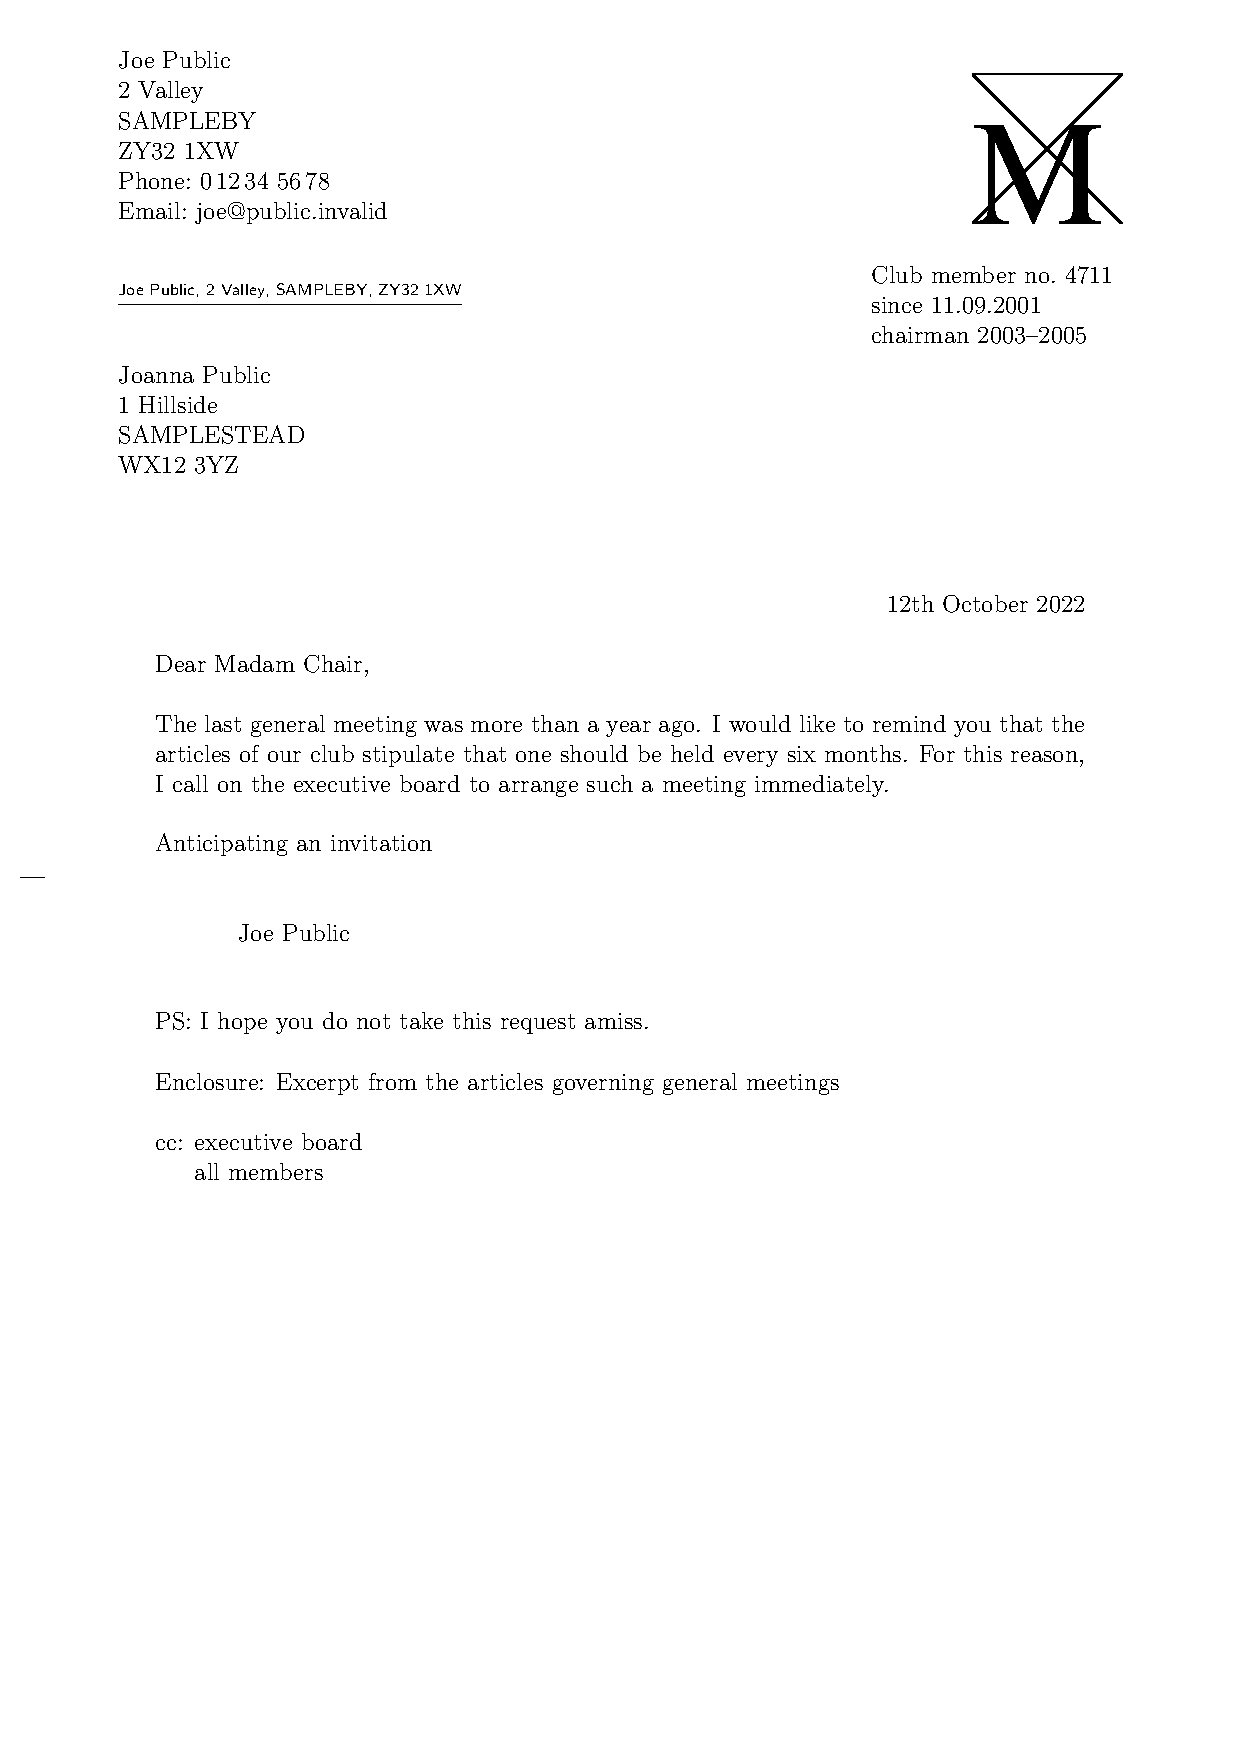
\includegraphics[width=.4\textwidth]{letter-example-19-en}}
    \end{captionbeside}
    \label{fig:\LabelBase.letter-19}
  \end{figure}
\end{Example}
\EndIndexGroup
\EndIndexGroup


\begin{Declaration}
  \PLength{locheight}%
  \PLength{lochpos}%
  \PLength{locvpos}%
  \PLength{locwidth}
\end{Declaration}
The \PLength{locwidth} and
\PLength{locheight}\ChangedAt{v2.97d}{\Class{scrlttr2}} pseudo-lengths set the
width and height of the extra-sender-information field. The \PLength{lochpos}
and \PLength{locvpos} pseudo-lengths determine the distances from the
top-right edge of the paper. These values are typically set to 0\Unit{pt} in
the predefined \File{lco} files. These\textnote{Attention!} zero-length values
have a special meaning. They result in the actual values being set within
\DescRef{\LabelBase.cmd.opening} based on the paper width, the address-window
width, the address window's distance from the top-left edge of the paper, and
the \DescRef{\LabelBase.option.locfield} option (see
\autoref{sec:\LabelBase.firstpage}, \DescPageRef{\LabelBase.option.locfield}). As
is the case for \PLength{toaddrhpos}, negative values of \PLength{lochpos}
also take on a special meaning. Instead of referring to the distance from the
right edge of the paper, \PLength{lochpos} then refers to the distance from
the left edge of the paper. The meaning is thus the opposite of that of
\PLength{toaddrhpos} (see \autoref{sec:\LabelBase.addressee},
\DescPageRef{\LabelBase.plength.toaddrhpos}).%
\EndIndexGroup
%
\EndIndexGroup


\subsection{Reference Line}
\seclabel{refLine}%
\BeginIndexGroup
\BeginIndex{}{reference line}
\index{business line|see{reference line}}

The reference line can actually be longer than just one line. It is printed
only if at least one of variables for the reference line is not empty. Only
non-empty fields will be printed. To\textnote{Hint!} set a seemingly empty
field, you can provide content for the variable that appears empty, such as
\Macro{mbox}\Parameter{}. If the reference line is omitted, the description
and contents of the \DescRef{\LabelBase.variable.date} variable are printed in
its place. You can find information about adding variables to or removing them
from the reference line in \autoref{sec:scrlttr2-experts.variables},
\DescPageRef{scrlttr2-experts.cmd.removereffields}.


\begin{Declaration}
  \OptionVName{numericaldate}{simple switch}
\end{Declaration}
This option toggles between the standard, language-dependent
date\Index{date}\Index{reference line} presentation, and a short, numerical
one. \KOMAScript{} does not provide the standard date format. It should be
defined by a package such as \Package{ngerman}\IndexPackage{ngerman},
\Package{babel}\IndexPackage{babel}, or
\Package{isodate}\IndexPackage{isodate}.
The\important{\OptionValue{numericaldate}{true}} short, numerical
representation, however, is produced by \Class{scrlttr2} itself. The option
recognizes the standard values for simple switches as listed in
\autoref{tab:truefalseswitch}, \autopageref{tab:truefalseswitch}. The default
is \PValue{false}, which results in standard date format.

\begin{Declaration}
  \Variable{date}%
\end{Declaration}
The date in the selected format is stored as \PName{content} of the
\Variable{date} variable. Setting the
\DescRef{\LabelBase.option.numericaldate} option has no effect if this
variable is overridden. The date is usually output as part of the reference
line. If all other elements of the reference line are empty, a date line
consisting of the location and the date is printed instead. However in this
case, the settings of the \DescRef{\LabelBase.option.refline} option described
below also affect the date line. See the description of variable
\DescRef{\LabelBase.variable.place} on
\DescPageRef{\LabelBase.variable.placeseparator} for more information about
the location.
%
\EndIndexGroup
\EndIndexGroup


\begin{Declaration}
  \OptionVName{refline}{selection}
\end{Declaration}
\BeginIndex{}{reference line}%
\index{business line|see{reference line}}%
Business letters in particular often contain an area with information such as
an identification code\Index{identification code}, phone
extension\Index{phone>extension}, customer number\Index{customer number},
invoice number\Index{invoice number}, or references to previous letters. This
guide calls this area the \emph{reference-field line}\textnote{reference-field
  line}, or simply the \emph{reference line}.

With \Class{scrlttr2} and  \Package{scrletter}, the header, footer, address,
and extra sender information can extend left and right beyond the normal
type area. The
\OptionValue{refline}{wide}\important{\OptionValue{refline}{wide}} option
specifies that this should also apply to the reference-field line. Normally,
the reference-field line contains at least the date, but it can hold
additional data. Available values for this option are shown in
\autoref{tab:\LabelBase.refline}. The default is \PValue{narrow} and
\PValue{dateright}\ChangedAt{v3.09}{\Class{scrlttr2}}.%
%
\begin{table}
  \caption[{Available values for the \Option{refline} option with
    \Class{scrlttr2}}]{Available values for the \Option{refline} option to set
    the width of the reference line with \Class{scrlttr2}}
  \label{tab:\LabelBase.refline}
  \begin{desctabular}
    \pventry{dateleft}{\ChangedAt{v3.09}{\Class{scrlttr2}}%
      The date is placed leftmost in the reference line.}%
    \pventry{dateright}{\ChangedAt{v3.09}{\Class{scrlttr2}}%
      The date is placed rightmost in the reference line.}%
    \pventry{narrow}{The reference line is restricted to the type area.}%
    \pventry{nodate}{\ChangedAt{v3.09}{\Class{scrlttr2}}%
      The date is not placed automatically into the reference line.}%
    \pventry{wide}{The width of the reference line depends on the positions of
      the address and extra sender information.}%
  \end{desctabular}
\end{table}

\begin{Declaration}
  \Variable{yourref}%
  \Variable{yourmail}%
  \Variable{myref}%
  \Variable{customer}%
  \Variable{invoice}%
\end{Declaration}
You can manage the typical contents of the reference-field line with five
variables: \Variable{yourref}, \Variable{yourmail}, \Variable{myref},
\Variable{customer} and \Variable{invoice}. Their meanings are listed in
\autoref{tab:\LabelBase.variables} on \autopageref{tab:\LabelBase.variables}.
Each variable has also a predefined \PName{description}, shown in
\autoref{tab:\LabelBase.reflineTerm}. How to add more variables to the
reference-field line is explained in \autoref{sec:scrlttr2-experts.variables}
starting on \DescPageRef{scrlttr2-experts.cmd.newkomavar}.%
%
\begin{table}
%  \centering
  \KOMAoptions{captions=topbeside}%
  \setcapindent{0pt}%
%  \caption
  \begin{captionbeside}[{Default descriptions of variables in the
      reference line}]{Default descriptions of typical variables in the
      reference line using language-dependent commands}%
    [l]
  \begin{tabular}[t]{lll}
    \toprule
    name                & description    & English default text\\
    \midrule
    \Variable{yourref}  & \DescRef{scrlttr2-experts.cmd.yourrefname}  & Your reference \\
    \Variable{yourmail} & \DescRef{scrlttr2-experts.cmd.yourmailname} & Your letter from \\
    \Variable{myref}    & \DescRef{scrlttr2-experts.cmd.myrefname}    & Our reference \\
    \Variable{customer} & \DescRef{scrlttr2-experts.cmd.customername} & Customer No.: \\
    \Variable{invoice}  & \DescRef{scrlttr2-experts.cmd.invoicename}  & Invoice No.: \\
    \DescRef{\LabelBase.variable.date} & \DescRef{scrlttr2-experts.cmd.datename} & date \\
    \bottomrule
  \end{tabular}
  \end{captionbeside}
  \label{tab:\LabelBase.reflineTerm}
\end{table}

\BeginIndexGroup
\BeginIndex{FontElement}{refname}\LabelFontElement{refname}%
\BeginIndex{FontElement}{refvalue}\LabelFontElement{refvalue}%
You\ChangedAt{v2.97c}{\Class{scrlttr2}} can change the font style and colour
of the \PName{description} and \PName{content} of the fields in the reference
line with the \FontElement{refname}%
\important[i]{\FontElement{refname}\\\FontElement{refvalue}} and
\FontElement{refvalue} elements using the \DescRef{\LabelBase.cmd.setkomafont}
and \DescRef{\LabelBase.cmd.addtokomafont} commands (see
\autoref{sec:\LabelBase.textmarkup},
\DescPageRef{\LabelBase.cmd.setkomafont}). The defaults for both elements are
listed in \autoref{tab:\LabelBase.refnamerefvalue}.%
\begin{table}[tp]
%  \centering
  \KOMAoptions{captions=topbeside}%
  \setcapindent{0pt}%
%  \caption
  \begin{captionbeside}
    [{Default font styles for elements in the reference line}]{Default font
      style settings for the elements in the reference line%
      \label{tab:\LabelBase.refnamerefvalue}}
    [l]
    \begin{tabular}[t]{ll}
      \toprule
      element & default configuration \\
       \midrule
      \ChangedAt{v3.39}{\Class{scrlttr2}}%
      \DescRef{\LabelBase.fontelement.refname}
              & \DescRef{\LabelBase.cmd.maybesffamily}\IndexCmd{maybesffamily}%
                \Macro{scriptsize} \\
      \DescRef{\LabelBase.fontelement.refvalue} & \\
      \bottomrule
    \end{tabular}
  \end{captionbeside}
\end{table}%
%
\EndIndexGroup


\begin{Declaration}
  \Variable{placeseparator}%
\end{Declaration}%
\BeginIndex{Variable}{place}%
If all variables in the reference-field line, with the exception of
\DescRef{\LabelBase.variable.date}%
\important{\DescRef{\LabelBase.variable.date}}\IndexVariable{date}, are empty,
no actual reference line is output. Instead, a date line consisting only of a
location\Index{location} and a date\Index{date} is output. The \PName{content}
of the \DescRef{\LabelBase.variable.place} variable contains the location. The
delimiter, which in this case is placed after the location, is specified by
the \PName{content} of the \Variable{placeseparator} variable. The
default\textnote{default} \PName{content} of the delimiter is a comma followed
by a non-breaking space. If the location is empty, the delimiter is not
output. The default \PName{content} of \DescRef{\LabelBase.variable.date} is
\Macro{today}\IndexCmd{today} and depends on the setting of the
\DescRef{\LabelBase.option.numericaldate} option (see
\DescPageRef{\LabelBase.option.numericaldate}).

Starting with version~3.09\ChangedAt{v3.09}{\Class{scrlttr2}}, the location
and date are no longer required to be right-aligned. Instead, when a date
line is used, its alignment is specified by the date setting of the
\DescRef{\LabelBase.option.refline} option, as listed in
\autoref{tab:\LabelBase.refline}.

\BeginIndexGroup
\BeginIndex{FontElement}{placeanddate}\LabelFontElement{placeanddate}%
If\ChangedAt{v3.12}{\Class{scrlttr2}} such a date line is output with a
location rather than a reference-field line, the font setting of the
\DescRef{\LabelBase.fontelement.refvalue} element does not apply. In this
case, the \FontElement{placeanddate}\important{\FontElement{placeanddate}}
element is used. You can change the empty default of this font element as
usual with the \DescRef{\LabelBase.cmd.setkomafont} and
\DescRef{\LabelBase.cmd.addtokomafont} commands (see
\autoref{sec:\LabelBase.textmarkup},
\DescPageRef{\LabelBase.cmd.setkomafont}).%
\EndIndexGroup

\begin{Example}
  Now Mr Public also sets the variable for the location:%
  \lstinputcode[xleftmargin=1em]{letter-example-20-en.tex}%
  As seen in \autoref{fig:\LabelBase.letter-20}, the location appears
  in front of the date, followed by the automatic delimiter. This date has
  been defined explicitly so that the original date is maintained in any later
  \LaTeX{} run rather than using the date of the \LaTeX{} run.
  \begin{figure}
    \setcapindent{0pt}%
    \begin{captionbeside}[{Example: letter with extended sender, logo,
        recipient, extra sender information, location, date, opening,
        text, closing, signature, postscript, distribution list, enclosure,
        and hole-punch mark}]
      {result of a short letter with extended sender, logo, recipient,
        extra sender information, location, date, opening, text, closing,
        signature, postscript, distribution list, enclosure and hole-punch
        mark}[l]
      \frame{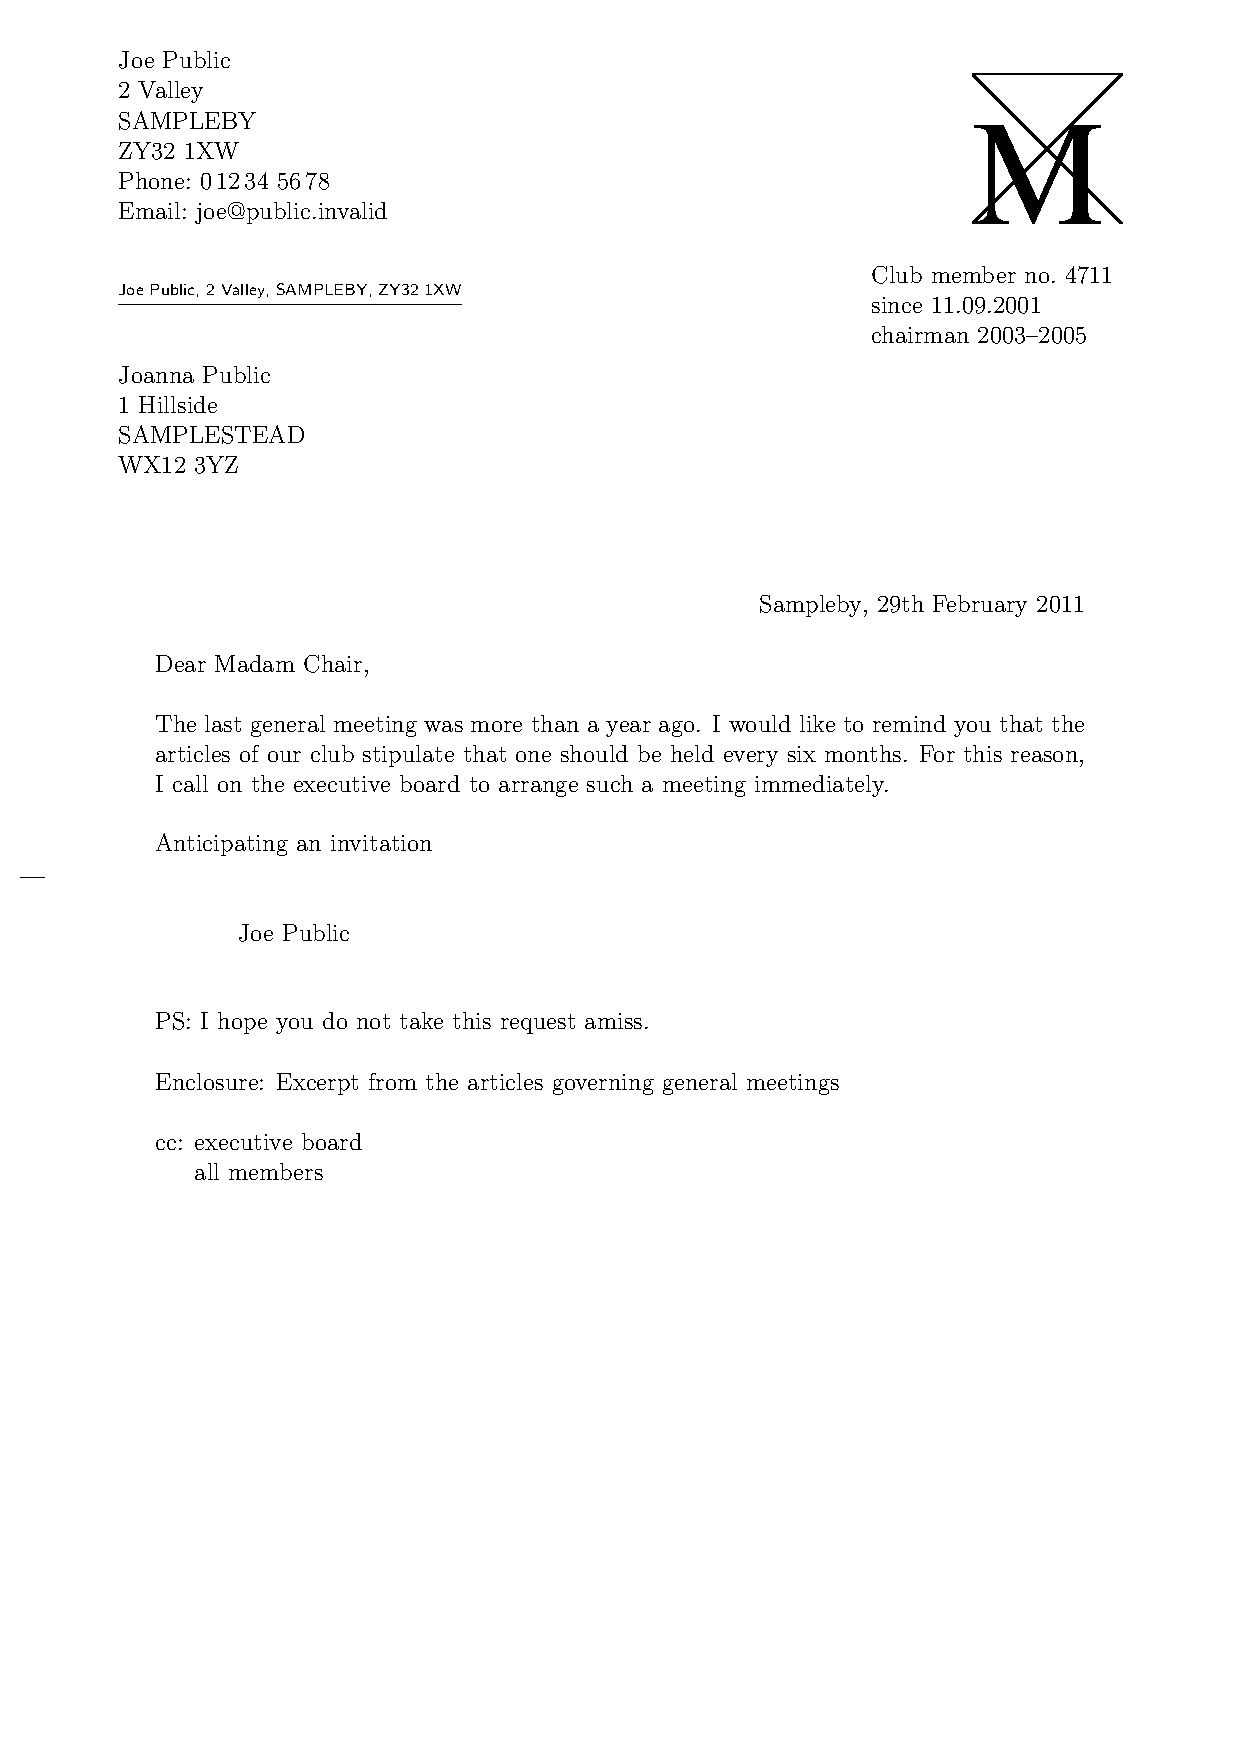
\includegraphics[width=.4\textwidth]{letter-example-20-en}}
    \end{captionbeside}
    \label{fig:\LabelBase.letter-20}
  \end{figure}
\end{Example}
%
\EndIndexGroup
\EndIndexGroup
\EndIndexGroup


\begin{Declaration}
  \PLength{refvpos}
\end{Declaration}
This pseudo-length specifies the distance from the upper edge of the paper to
the reference line. Its value is set differently in the various predefined
\File{lco} files\textnote{\File{lco} file}\Index{lco file=\File{lco} file}.
Typical values are between 80.5\Unit{mm} and 98.5\Unit{mm}.%
\EndIndexGroup


\begin{Declaration}
  \PLength{refwidth}%
  \PLength{refhpos}
\end{Declaration}
The \PLength{refwidth} pseudo-length specifies the width available for the
reference line. Its value is typically set to 0\Unit{pt} in the predefined
\File{lco} files\textnote{\File{lco} file}\Index{lco file=\File{lco} file}.
This\textnote{Attention!} value has a special meaning. In no way does it
indicate that there is no available width for the reference line. Instead, it
indicates that the width will be calculated within the
\DescRef{\LabelBase.cmd.opening}\IndexCmd{opening} command. This calculated
width then depends on the value of the \DescRef{\LabelBase.option.refline}%
\important{\DescRef{\LabelBase.option.refline}}%
\IndexOption{refline~=\PName{setting}} options (see
\autoref{sec:\LabelBase.firstpage}, \DescPageRef{\LabelBase.option.refline}). At
the same time, \PLength{refhpos} will also be set according to this option.
With \OptionValueRef{scrlttr2}{refline}{wide}%
\IndexOption{refline~=\textKValue{wide}}, the reference fields line is
centred, while with \OptionValueRef{scrlttr2}{refline}{narrow}%
\IndexOption{refline~=\textKValue{narrow}} it is aligned flush left with the
type area.

If \PLength{refwidth} is not zero, the width of the reference line is not
determined by the  \DescRef{\LabelBase.option.refline} option, and so
\PLength{refhpos} specifies the distance of the reference line from the left
edge of the paper. If\textnote{Attention!} this distance is zero, the the
reference line is placed so that the ratio between its distances from the left
and right edges of the paper corresponds to the ratio of distance of the type
area from the left and right edges of the paper. Thus, for a type area
horizontally centred on the paper, the reference line will also be centred.

As a rule, these special cases are likely of little interest to the normal
user. The\textnote{Attention!} simplest rule is as follows: either
\PLength{refhpos} remains zero, and so the width and alignment of the
reference line are determined with the \DescRef{\LabelBase.option.refline}
option, or the user sets both \PLength{refwidth} and \PLength{refhpos}.%
\EndIndexGroup


\begin{Declaration}
  \PLength{refaftervskip}
\end{Declaration}
This pseudo-length specifies the vertical skip to be inserted beneath the
reference line. The value is set in the predefined \File{lco}
files\textnote{\File{lco} file}\Index{lco file=\File{lco} file}. It directly
affects the height of the text area on the first page. A typical value is
between one and two lines.%
\EndIndexGroup
%
\EndIndexGroup


\subsection{Subject}
\seclabel{subject}%
\BeginIndexGroup
\BeginIndex{}{subject}

Different countries have different conventions for placing the subject line of
a letter. Some place it before the opening phrase; others place it after. Some
professional groups even want it before the reference line.


\begin{Declaration}
  \Variable{title}%
\end{Declaration}
With \KOMAScript{}, you can also give a letter a title\Index{title}. The title
is centred, using the \Macro{LARGE} font size, and placed directly beneath the
reference-field line.

\BeginIndex{FontElement}{lettertitle}\LabelFontElement{lettertitle}%
\BeginIndex{FontElement}{title}\LabelFontElement{title}%
You can change the font style for the
\FontElement{lettertitle}\important{\FontElement{lettertitle}} element with
the \DescRef{\LabelBase.cmd.setkomafont} and
\DescRef{\LabelBase.cmd.addtokomafont} commands (see
\autoref{sec:\LabelBase.textmarkup},
\DescPageRef{\LabelBase.cmd.setkomafont}). Font size declarations are
allowed. The \Macro{LARGE} font size always precedes the font selection in
\KOMAScript{}, and is therefore not part of the default setting
\ChangedAt{v3.39}{\Class{scrlttr2}}\Macro{normalcolor}\linebreak[2]%
\DescRef{\LabelBase.cmd.maybesffamily}\IndexCmd{maybesffamily}\linebreak[2]%
\Macro{bfseries}. With \Class{scrlttr2},
you can also use \FontElement{title}\important{\FontElement{title}} as an
alias for \FontElement{lettertitle}. This is not possible when using
\Package{scrletter} with a \KOMAScript{} class because these classes already
define a \FontElement{title} element for the document title with different
setting.%
\EndIndex{FontElement}{title}%
\EndIndex{FontElement}{lettertitle}%
\begin{Example}
  Suppose you are writing a reminder letter. You set a corresponding title:
\begin{lstlisting}
  \setkomavar{title}{Reminder}
\end{lstlisting}
  This way the recipient should recognize the reminder as such.
\end{Example}
As shown in the example, the \PName{content} of the variable defines the
title. \KOMAScript{} does not use the \PName{description}.%
%
\EndIndexGroup


\begin{Declaration}
  \OptionVName{subject}{selection}%
  \Variable{subject}%
  \Variable{subjectseparator}%
\end{Declaration}
\BeginIndex{}{subject}%
To include a subject, define the \PName{content} of the \Variable{subject}
variable accordingly. First of all, you can use the
\OptionValue{subject}{true}\important{\OptionValue{subject}{titled}} option,
to choose whether the subject should be preceded with a \PName{description} or
not. If you use the \PName{description} the \PName{content} of the
\Variable{subjectseparator}\Index{separator} variable is output between the
\PName{description} and the \PName{content} of the \Variable{subject}
variable. The default \PName{content} of \PName{subjectseparator} consists of
a colon followed by a space.

\begin{table}
%  \centering
  \KOMAoptions{captions=topbeside}%
  \setcapindent{0pt}%
%  \caption
  \begin{captionbeside}{Default descriptions of variables for the subject}
    [l]
    \begin{tabular}[t]{lll}
      \toprule
      variable name      & description \\
      \midrule
      \Variable{subject} & \DescRef{\LabelBase.cmd.usekomavar*}\PParameter{subjectseparator}%
                           \texttt{\%} \\ 
                         & \texttt{\quad}%
                           \DescRef{\LabelBase.cmd.usekomavar}\PParameter{subjectseparator} \\
      \Variable{subjectseparator} & \DescRef{scrlttr2-experts.cmd.subjectname} \\
      \bottomrule
    \end{tabular}
  \end{captionbeside}
  \label{tab:\LabelBase.subjectTerm}
\end{table}

Additionally, you can use \OptionValue{subject}{afteropening}%
\important{\OptionValue{subject}{afteropening}\\
  \OptionValue{subject}{beforeopening}} to place the subject after the letter
opening instead of the default \OptionValue{subject}{beforeopening}. You can
also specify other formatting\important{\OptionValue{subject}{underlined}\\
  \OptionValue{subject}{centered}\\
  \OptionValue{subject}{right}} for the subject with
\OptionValue{subject}{underlined}, \OptionValue{subject}{centered}, or
\OptionValue{subject}{right}\ChangedAt{v2.97c}{\Class{scrlttr2}}. The
available values are listed in \autoref{tab:\LabelBase.subject}.
Note\textnote{Attention!} that with the \OptionValue{subject}{underlined}
option, the whole subject must fit onto one line. The defaults are
\OptionValue{subject}{left}, \OptionValue{subject}{beforeopening}, and
\OptionValue{subject}{untitled}.%
%
\begin{table}
%  \centering
  \KOMAoptions{captions=topbeside}%
  \setcapindent{0pt}%
%  \caption
  \begin{captionbeside}
    [{Available values for the \Option{subject} option with \Class{scrlttr2}}]
    {Available values for the \Option{subject} option for the position and
      formatting of the subject with
      \Class{scrlttr2}\label{tab:\LabelBase.subject}}%
    [l]
    \begin{minipage}[t]{.6\linewidth}
      \begin{desctabular}[t]
        \pventry{afteropening}{subject after opening}%
        \pventry{beforeopening}{subject before opening}%
        \pventry{centered}{subject centred}%
        \pventry{left}{subject left-justified}%
        \pventry{right}{subject right-justified}%
        \pventry{titled}{add title/description to subject}%
        \pventry{underlined}{set subject underlined (see note in text)}%
        \pventry{untitled}{do not add title/description to subject}%
      \end{desctabular}
    \end{minipage}
  \end{captionbeside}
\end{table}

\BeginIndexGroup
\BeginIndex{FontElement}{lettersubject}\LabelFontElement{lettersubject}%
\BeginIndex{FontElement}{subject}\LabelFontElement{subject}%
The subject line is set in a separate font\Index{font>style}. To change this,
use the \DescRef{\LabelBase.cmd.setkomafont} and
\DescRef{\LabelBase.cmd.addtokomafont} commands (see
\autoref{sec:\LabelBase.textmarkup},
\DescPageRef{\LabelBase.cmd.setkomafont}). For the
\FontElement{lettersubject}\important{\FontElement{lettersubject}} element,
the default font is \Macro{normalcolor}\Macro{bfseries}. With the
\Class{scrlttr2} class, you can also use
\FontElement{subject}\important{\FontElement{subject}} as an alias of
\FontElement{lettersubject}. This is not possible with the \Package{scrletter}
package when using a \KOMAScript{} class, because these classes already define
a \FontElement{subject} element for the document title with different
settings.%
\EndIndexGroup

\begin{Example}
  Mr Public now includes a subject. As a traditionalist, he also wants the
  subject to be labelled accordingly and therefore sets the corresponding
  option:%
  \lstinputcode[xleftmargin=1em]{letter-example-21-en.tex}%
  The result is shown in \autoref{fig:\LabelBase.letter-21}.
  \begin{figure}
    \setcapindent{0pt}%
    \begin{captionbeside}[{Example: letter with extended sender, logo,
        recipient, extra sender information, place, date, subject,
        opening, text, closing, signature, postscript, distribution list,
        enclosure, and hole-punch mark}]
      {result of a short letter with extended sender, logo, recipient,
        extra sender information, place, date, subject, opening, text,
        closing, signature, postscript, distribution list, enclosure and
        hole-punch mark}[l]
      \frame{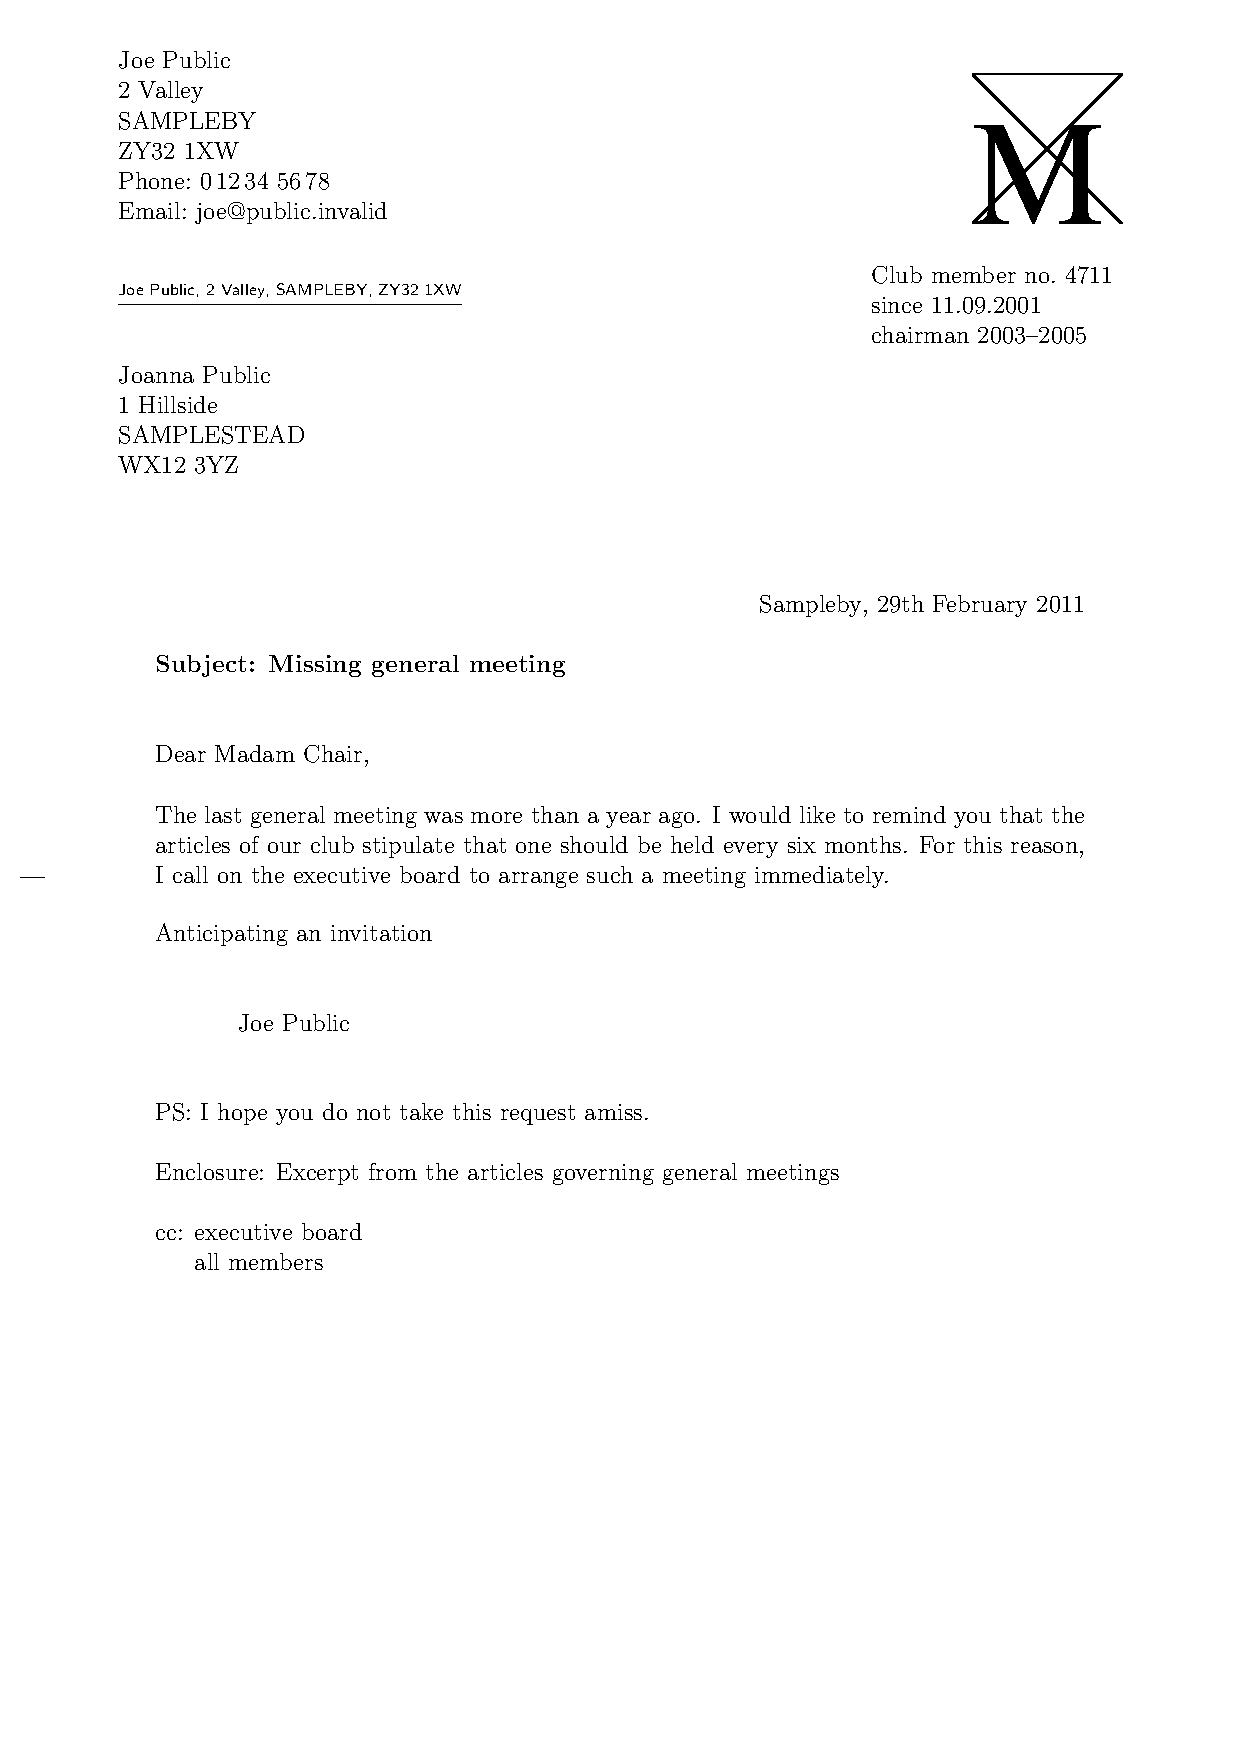
\includegraphics[width=.4\textwidth]{letter-example-21-en}}
    \end{captionbeside}
    \label{fig:\LabelBase.letter-21}
  \end{figure}
\end{Example}
%
\EndIndexGroup


\begin{Declaration}
  \PLength{subjectvpos}
\end{Declaration}
\ChangedAt{v3.01}{\Class{scrlttr2}}%
If\textnote{Attention!} the value of this pseudo-length is 0\Unit{pt}, the
\DescRef{\LabelBase.option.subject}\important{\DescRef{\LabelBase.option.subject}}%
\IndexOption{subject~=\PName{Einstellung}} option (see
\autoref{sec:\LabelBase.firstpage}, \DescPageRef{\LabelBase.option.subject})
determines the position of the subject. Any other value defines the distance
between the top edge of the paper and the subject. In this
case\textnote{Hint!}, you should ensure that there is enough space available
that overlapping with other elements is unlikely.
\begin{Example}
  A few professionals prefer to have the subject above the reference line. For
  this, you can specify the position as follows, which also changes the
  position of the reference line itself:
\begin{lstcode}
  \ProvidesFile{lawsubj.lco}
               [2008/11/03 lawyers lco file]
  \setplength{subjectvpos}{\useplength{refvpos}}
  \addtoplength{refvpos}{3\baselineskip}
  \endinput
\end{lstcode}
  If you want to leave at least one empty line between the subject and the
  reference, you have space for a maximum of two lines.
\end{Example}
\EndIndexGroup


\begin{Declaration}
  \PLength{subjectbeforevskip}%
  \PLength{subjectaftervskip}
\end{Declaration}
\ChangedAt{v3.01}{\Class{scrlttr2}}%
If the subject is placed not absolutely but before or after the salutation,
you can insert additional vertical space before and after the subject. The
space before the subject may interfere with other distances, such as the
automatic distance of one line after the title. Therefore the default is to
use no additional space here. The default of the class and the package for the
space after the subject is two lines.%
\EndIndexGroup
%
\EndIndexGroup


\subsection{Closing}
\seclabel{closing}
\BeginIndexGroup
\BeginIndex{}{closing}

\BeginIndex{}{letter>closing}%
\BeginIndex{}{signature}%
\BeginIndex{}{letter>signature}%

It has already been mentioned in \autoref{sec:\LabelBase.document},
\DescPageRef{\LabelBase.cmd.closing} that the letter's closing text is
provided by \DescRef{\LabelBase.cmd.closing}\IndexCmd{closing}. Beneath the
closing text, there is often a space for a handwritten signature, beneath
which there can be a printed name, which serves as a kind of annotation to the
actual signature.


\begin{Declaration}
  \Variable{signature}%
\end{Declaration}
The \Variable{signature} variable contains the printed name or annotation for
the handwritten signature. Its default \PName{content} is the
\DescRef{\LabelBase.cmd.usekomavar}\PParameter{fromname}. This annotation can
consist of multiple lines. In that case, you should separate the individual
lines with double backslashes. Paragraph\textnote{Attention!} breaks in the
signature annotation, however, are not permitted.%
\EndIndexGroup


\begin{Declaration}
  \Macro{raggedsignature}
\end{Declaration}
The closing phrase and the signature will be typeset in a box. The width of
the box is determined by the length of the longest line in the closing
phrase or signature.

The \PLength{sigindent}\IndexPLength{sigindent} and
\PLength{sigbeforevskip}\IndexPLength{sigbeforevskip} pseudo-lengths determine
exactly where this box is placed (see \autoref{sec:\LabelBase.closing},
\DescPageRef{\LabelBase.plength.sigindent}). The \Macro{raggedsignature}
command defines the alignment inside the box. In the default \File{lco} files,
the command is either defined as \Macro{centering} (all besides
\Option{KOMAold}) or \Macro{raggedright} (\Option{KOMAold}). In order to
obtain flush-right or flush-left alignment inside the box, you can redefine
the command in the same way as \DescRef{maincls.cmd.raggedsection} (see the
example in \autoref{sec:maincls.structure},
\DescPageRef{maincls.cmd.raggedsection}).

\begin{Example}
  Now Mr Public wants to make himself seem really important, and therefore he uses the
  signature to show once again that he was formerly a chairman himself. So
  he changes \PName{contents} of the
  \DescRef{\LabelBase.variable.signature} variable. He also wants the signature
  be aligned flush-left and so he also redefines \Macro{raggedsignature}:%
  \lstinputcode[xleftmargin=1em]{letter-example-22-en.tex}%
  See \autoref{fig:\LabelBase.letter-22} for the result.
  \begin{figure}
    \setcapindent{0pt}%
    \begin{captionbeside}[{Example: letter with extended sender, logo,
        recipient, extra sender information, place, date, subject,
        opening, text, closing, modified signature, postscript, distribution
        list, enclosure, and hole-punch mark}]
      {result of a short letter with extended sender, logo, recipient,
        extra sender information, place, date, subject opening, text,
        closing, modified signature, postscript, distribution list, enclosure
        and hole-punch mark}[l]
      \frame{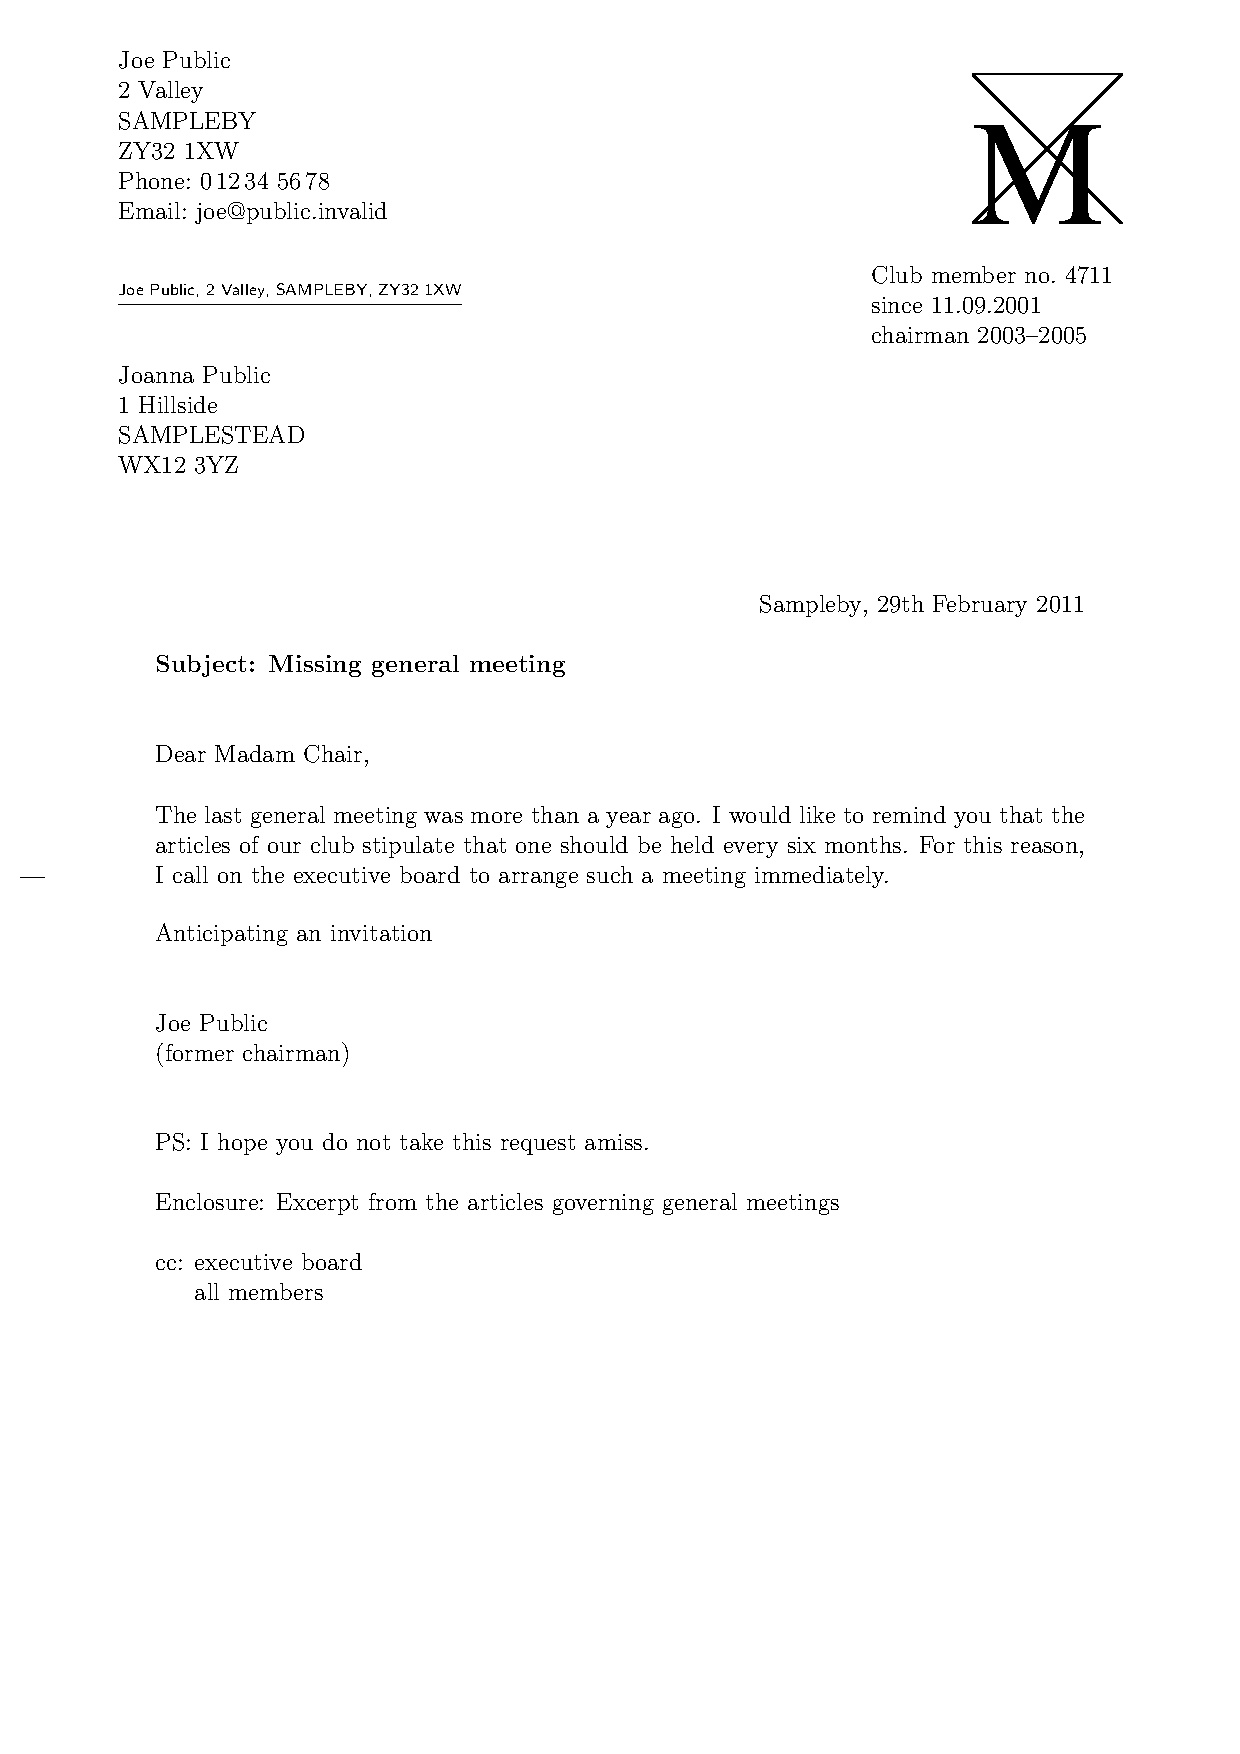
\includegraphics[width=.4\textwidth]{letter-example-22-en}}
    \end{captionbeside}
    \label{fig:\LabelBase.letter-22}
  \end{figure}
\end{Example}
\iftrue% Umbruchkorrekturtext
  The preceding example shows the most important, although not all possible,
  elements of a letter. It can, however, serve quite well as a general
  template.%
\else
  \vskip -1\ht\strutbox plus .75\ht\strutbox% example at end of description
\fi
%
\EndIndexGroup


\begin{Declaration}
  \PLength{sigindent}%
  \PLength{sigbeforevskip}
\end{Declaration}
The closing phrase\Index{closing>phrase}\Index{signature} and signature
explanation are typeset in a box whose width is determined by the length of
the longest line of the closing phrase or explanation.

The box will be indented by the distance specified in the \PLength{sigindent}
pseudo-length. In the predefined \File{lco} files\textnote{\File{lco}
file}\Index{lco file=\File{lco} file}, this length is set to 0\Unit{mm}.

Between the closing phrase and the signature explanation, a vertical skip is
inserted whose height is defined in the \PLength{sigbeforevskip}
pseudo-length. In the predefined \File{lco} files\textnote{\File{lco}
file}\Index{lco file=\File{lco} file} this value is set to two lines. In this
space you can then write your signature.%
\iffalse% Umbruchkorrekturtext
\ If you decide to include a facsimile of your signature in the
\DescRef{\LabelBase.variable.signature}\IndexVariable{signature}%
\important{\DescRef{\LabelBase.variable.signature}} with the
\Package{graphicx}\IndexPackage{graphicx} package, it would be useful
to reduce the value of \PLength{sigbeforevskip} and thus the gap between
the closing phrase and the signature.%
\fi%
\EndIndexGroup
%
\EndIndexGroup


\subsection{Letterhead Page Footer}
\seclabel{firstFoot}%
\BeginIndexGroup
\BeginIndex{}{letterhead page>footer}%

The first page of a letter, the letterhead page, contains not just its own
header, the letterhead, but also its own footer\Index{footer>letterhead
page}\Index{footer}. Just like the letterhead, it will be set not by the page
style but directly within \DescRef{\LabelBase.cmd.opening}\IndexCmd{opening}%
\important{\DescRef{\LabelBase.cmd.opening}}.


\begin{Declaration}
  \OptionVName{enlargefirstpage}{simple switch}
\end{Declaration}
\begin{Explain}
  The first page of a letter always uses a different page layout because of
  the many predefined elements such as the letterhead or the address. The
  \Class{scrlttr2} class provides a mechanism to calculate height and vertical
  alignment of header and footer of the first page independently of the
  subsequent pages. If, as a result, the footer of the first page would
  protrude into the text area, this text area of the first page is
  automatically reduced using
  \Macro{enlargethispage}\IndexCmd{enlargethispage}.
\end{Explain}
If the text area should become larger, assuming the footer on the first page
permits this, you can use this option. At best, a little more text will then
fit on the first page. See also the description of the \PLength{firstfootvpos}
pseudo-length on \DescPageRef{\LabelBase.plength.firstfootvpos}.  This
option takes the standard values for simple switches, as listed in
\autoref{tab:truefalseswitch}, \autopageref{tab:truefalseswitch}. The default
is \PValue{false}.\textnote{default}%
\EndIndexGroup


\begin{Declaration}
  \OptionVName{firstfoot}{simple switch}
\end{Declaration}
\BeginIndex{}{letterhead page>footer}%
This\ChangedAt{v2.97e}{\Class{scrlttr2}} option determines whether the footer
for the letterhead page is output. Switching off the letterhead page footer
with \OptionValue{firstfoot}{false}\important{\OptionValue{firstfoot}{false}},
has an effect when the \DescRef{\LabelBase.option.enlargefirstpage} option 
(see \DescPageRef{\LabelBase.option.enlargefirstpage}) is used at the same
time, as this will logically extend the page downwards. In this case, the
distance that is ordinarily between type area and the footer becomes the
distance between the end of the type area and the bottom of the page.

The option recognizes the standard values for simple switches listed in
\autoref{tab:truefalseswitch}, \autopageref{tab:truefalseswitch}. The default
is to include the letterhead page footer.
\EndIndexGroup


\begin{Declaration}
  \Variable{firstfoot}%
\end{Declaration}%
\BeginIndex{}{letterhead page>footer}%
The footer of the first page is empty by default.
However\ChangedAt{v3.08}{\Class{scrlttr2}}, you can specify a new footer
in the \PName{content} of the \Variable{firstfoot} variable. \KOMAScript{}
does not use the \PName{description} of the variable.

\BeginIndex{Variable}{frombank}%
\begin{Example}
  You want to put the \PName{content} of the \Variable{frombank} variable
  (i.\,e. the bank account details) in the footer of the first page. The
  double backslash should be replaced with a comma:
\begin{lstcode}
  \setkomavar{firstfoot}{%
    \parbox[b]{\linewidth}{%
      \centering\def\\{, }\usekomavar{frombank}%
    }%
  }
\end{lstcode}
  You can also define your own variable for the separator. I leave
  this as an exercise for the reader.

  If you want to create a footer in order to counterbalance the letterhead, you
  can do so, for example, as follows:
\begin{lstcode}
  \setkomavar{firstfoot}{%
    \parbox[t]{\textwidth}{\footnotesize
      \begin{tabular}[t]{l@{}}%
        \multicolumn{1}{@{}l@{}}{Partners:}\\
        Jim Smith\\
        Russ Mayer
      \end{tabular}%
      \hfill
      \begin{tabular}[t]{l@{}}%
        \multicolumn{1}{@{}l@{}}{Managing Director:}\\
        Lisa Mayer\\[1ex]
        \multicolumn{1}{@{}l@{}}{Court Jurisdiction:}\\
        Great Plains
      \end{tabular}%
      \Ifkomavarempty{frombank}{}{%
        \hfill
        \begin{tabular}[t]{l@{}}%
          \multicolumn{1}{@{}l@{}}{\usekomavar*{frombank}:}\\
          \usekomavar{frombank}
        \end{tabular}%
      }%
    }%
  }
\end{lstcode}
  This example originally came from Torsten Kr\"uger. You should
  consider placing a definition intended for multiple use in different
  documents in a separate \File{lco} file\Index{lco file=\File{lco} file}.
\begin{lstcode}
  \setkomavar{frombank}{Account No. 12345678\\
    Buffoon Bank\\
    Bank Code: 65-43-21}
\end{lstcode}
  can then be used to set the bank details in the document.
%  However depending on your settings, there may not be sufficient space
%  for such a large footer, and it may therefore be placed too low on the
%  page. In such a case, you can adjust its vertical position with the
%  pseudo-length \PLength{firstfootvpos}\IndexPLength{firstfootvpos}.
\end{Example}

The previous example uses a multi-line footer.  With a compatibility setting
of version 2.9u (see \DescRef{\LabelBase.option.version} in
\autoref{sec:\LabelBase.compatibilityOptions},
\DescPageRef{\LabelBase.option.version}) the space is generally insufficient.
In this case, you should reduce \PLength{firstfootvpos} (see
\DescPageRef{\LabelBase.plength.firstfootvpos}) appropriately.%
\EndIndexGroup

\begin{Declaration}
  \Variable{frombank}
\end{Declaration}%
\BeginIndex{}{letterhead page>footer}%
The \Variable{frombank} variable used in the previous example
occupies a special position. It is not currently used internally. However, you
can use it to put the bank information\Index{bank information} in the
extra sender information field or in the footer, as in the example (see
the variable \DescRef{\LabelBase.variable.location},
\DescPageRef{\LabelBase.variable.location}).%
%
\EndIndexGroup


\begin{Declaration}
  \PLength{firstfootvpos}
\end{Declaration}
This pseudo-length gives the distance from the top of the paper to the footer
of the letterhead page. It also ensures that the text area does not protrude
into the footer. To do so, the height of the text area on the first page will
be decreased, if necessary, using
\Macro{enlargethispage}\IndexCmd{enlargethispage}%
\important{\Macro{enlargethispage}}. The
\DescRef{\LabelBase.option.enlargefirstpage}%
\important{\DescRef{\LabelBase.option.enlargefirstpage}} option (see
\autoref{sec:\LabelBase.firstpage},
\DescPageRef{\LabelBase.option.enlargefirstpage}) can also ensure that the
height of the text area is increased, if necessary. Thus, the distance between
text area and the letterhead page footer can be reduced to the value of the
\Length{footskip}\IndexLength{footskip}\important{\Length{footskip}} length.

With\textnote{Attention!} the compatibility option
set\ChangedAt{v2.9t}{\Class{scrlttr2}} to versions up to
2.9t\IndexOption{version~=\PValue{2.9t}} (see
\DescRef{\LabelBase.option.version} in
\autoref{sec:\LabelBase.compatibilityOptions},
\DescPageRef{\LabelBase.option.version}) the footer is set independently of the
type area in all predefined \File{lco} files\textnote{\File{lco}
file}\Index{lco file=\File{lco} file} (see \autoref{sec:\LabelBase.lcoFile})
except for \Option{KOMAold} and \Option{NF}. Thus the
\DescRef{\LabelBase.option.enlargefirstpage}%
\important{\DescRef{\LabelBase.option.enlargefirstpage}} option has no effect.
From version 2.9u on, the footer is placed at the bottom edge of the paper.
Thus, the height of the letterhead page's type area may also depend on the
\DescRef{\LabelBase.option.enlargefirstpage} option.

If the letter footer is deactivated with the
\OptionValueRef{scrlttr2}{firstfoot}{false}%
\important{\OptionValueRef{scrlttr2}{firstfoot}{false}}%
\IndexOption{firstfoot~=\PValue{false}}\ChangedAt{v2.97e}{\Class{scrlttr2}}
option (see \autoref{sec:\LabelBase.firstpage},
\DescPageRef{\LabelBase.option.firstfoot}), the setting of
\PLength{firstfootvpos} is ignored, and instead
\Length{paperheight}\IndexLength{paperheight} is applied. There remains then a
minimum bottom margin of length \Length{footskip}\IndexLength{footskip}.%
\EndIndexGroup


\begin{Declaration}
  \PLength{firstfoothpos}
\end{Declaration}
\ChangedAt{v3.05}{\Class{scrlttr2}}%
A\textnote{Attention!} positive value of the \PLength{firstfoothpos}
pseudo-length specifies the distance from the left edge of the paper to the
letterhead page footer. If the value is greater than or equal to the paper
width, \Length{paperwidth}\IndexLength{paperwidth}, the footer is centred
horizontally on the letterhead page. But if the value is less than or equal to
the negative width of the paper, the footer is placed flush with the left edge
of the typing area.

The typical default for this value is \Length{maxdimen}\IndexLength{maxdimen},
which is the maximum possible value for a length. This results in horizontal
centring.%
\EndIndexGroup


\begin{Declaration}
  \PLength{firstfootwidth}
\end{Declaration}
This pseudo-length specifies the width of the footer of the first page of the
letter, that is the letterhead page. The value in the predefined \File{lco}
files\textnote{\File{lco} file}\Index{lco file=\File{lco} file} matches
\PLength{firstheadwidth}\important{\PLength{firstheadwidth}}%
\IndexPLength{firstheadwidth}.%
%
\EndIndexGroup
%
\EndIndexGroup
%
\EndIndexGroup

\LoadCommonFile{parmarkup} % \section{Paragraph Markup}

\LoadCommonFile{oddorevenpage} % \section{Detection of Odd and Even Pages}


\section{Headers and Footers with the Default Page Style}
\seclabel{pagestyle}
\BeginIndexGroup
\BeginIndex{}{page>style}%
\BeginIndex{}{page>header}%
\BeginIndex{}{page>footer}%

One of the general properties of a document is its page style. In \LaTeX{}
this mostly consists of the contents of headers and footers.
As\textnote{Attention!} already mentioned in
\autoref{sec:\LabelBase.firstpage}, the header and footer of the letterhead
page are treated as elements of the letterhead page. Therefore they do not
depend on the settings of the page style. So this section describes the page
styles of the subsequent pages of a letter after the letterhead page. For
one-sided letters, this is the page style of the second sheet. For two-sided
letters, this is also the page style of all verso pages.


\begin{Declaration}
  \Macro{letterpagestyle}
\end{Declaration}
The\ChangedAt{v3.19}{\Class{scrlttr2}\and \Package{scrletter}} default page
style for letters is specified by the contents of the \Macro{letterpagestyle}
command. By default\textnote{default},
\Class{scrlttr2}\OnlyAt{\Class{scrlttr2}} leaves this command empty. This
means that the page style of letters is the same as in the rest of the
document. This is useful because \Class{scrlttr2} is intended for letter-only
documents, and it is easier to define the page style for all letters globally,
using \DescRef{\LabelBase.cmd.pagestyle} as usual.

Since both the \DescRef{\LabelBase.pagestyle.plain} and the
\DescRef{\LabelBase.pagestyle.headings} page styles of other classes differs
from the page style necessary for letters, the
\Package{scrletter}\OnlyAt{\Package{scrletter}}\textnote{default} package
defines \Macro{letterpagestyle} with to be
\DescRef{\LabelBase.pagestyle.plain.letter}\IndexPagestyle{plain.letter}%
\important{\DescRef{\LabelBase.pagestyle.plain.letter}}. This causes all
letters to use the
\hyperref[desc:\LabelBase.pagestyle.plain.letter]{\PageStyle{plain}} style of
the \DescRef{\LabelBase.pagestyle.letter}\IndexPagestyle{letter} page style
pair, regardless of the page style of the rest of the document. See
\autoref{sec:scrlttr2-experts.pagestyleatscrletter} for more information about
the characteristics of the page style of the \Package{scrletter} package.
\begin{Example}
  You are using the \Package{scrletter} package and want letters to use the
  same page style that was set for the rest of the document with
  \DescRef{\LabelBase.cmd.pagestyle}. To do this, put the command
\begin{lstcode}
  \renewcommand*{\letterpagestyle}{}
\end{lstcode}
  in your document preamble. Notice the star in \Macro{renewcommand*}.
\end{Example}
Of course, if you use \DescRef{\LabelBase.cmd.pagestyle} or
\DescRef{\LabelBase.cmd.thispagestyle} inside a letter, this will take
precedence over the page style set in \Macro{begin}\PParameter{letter} with
\Macro{letterpagestyle}.%
\EndIndexGroup


\begin{Declaration}
  \OptionVName{headsepline}{simple switch}%
  \OptionVName{footsepline}{simple switch}
\end{Declaration}
With these options \Class{scrlttr2}\OnlyAt{scrlttr2} can select whether to put
a separator rule\Index{line>separator}\Index{rule>separator} below the header
or above the footer, respectively, on subsequent pages. This option acccepts
the standard values for simple switches listed in
\autoref{tab:truefalseswitch}, \autopageref{tab:truefalseswitch}.
Activating\important{\OptionValue{headsepline}{true}} the \Option{headsepline}
option enables a rule below the header.
Activating\important{\OptionValue{footsepline}{true}} the \Option{footsepline}
option enables a rule above the footer. Deactivating the options disables the
corresponding rules.

Of course, the \Option{headsepline} and \Option{footsepline} options have no
effect on the \DescRef{\LabelBase.pagestyle.empty}%
\important{\DescRef{\LabelBase.pagestyle.empty}} page style (see later in this
section). This page style explicitly does not use headers or footers.

Typographically\important{\DescRef{\LabelBase.pagestyle.headings}\\
  \DescRef{\LabelBase.pagestyle.myheadings}\\
  \DescRef{\LabelBase.pagestyle.plain}} speaking, such a rule creates an
optical effect of making the header or footer appear to be closer to the text
area. This does not mean that the distance between the header or footer and
the text should be increased. Instead, they should be seen as part of the text
body\Index{text>body} when calculating the type area. To achieve this
\Class{scrlttr2} uses the \Option{headsepline} class option to automatically
pass the \DescRef{typearea.option.headinclude}%
\important{\DescRef{typearea.option.headinclude}} package option to the
\hyperref[cha:typearea]{\Package{typearea}} package. The same applies to
\DescRef{\LabelBase.option.footsepline}  for
\DescRef{typearea.option.footinclude}%
\important{\DescRef{typearea.option.footinclude}}.

The options themselves do not automatically recalculate the type area. To
recalculate the type area, see the \DescRef{typearea.option.DIV} option with
the \PValue{last} or \PValue{current} values (see
\DescPageRef{typearea.option.DIV.last}), or the
\DescRef{typearea.cmd.recalctypearea} command (see
\DescPageRef{typearea.cmd.recalctypearea}) in \autoref{cha:typearea}.

The \hyperref[cha:scrlayer-scrpage]{\Package{scrlayer-scrpage}}%
\IndexPackage{scrlayer-scrpage}%
\important{\hyperref[cha:scrlayer-scrpage]{\Package{scrlayer-scrpage}}}
package (see \autoref{cha:scrlayer-scrpage}) provides further control over
header and footer rules and you can also combine it with \Class{scrlttr2}. The
\Package{scrletter} package automatically uses
\important{\hyperref[cha:scrlayer-scrpage]{\Package{scrlayer-scrpage}}} to
define the \DescRef{\LabelBase.pagestyle.letter} and
\DescRef{\LabelBase.pagestyle.plain.letter} page styles.

The\OnlyAt{\Package{scrletter}} \DescRef{\LabelBase.pagestyle.letter} and
\DescRef{\LabelBase.pagestyle.plain.letter} page styles defined by
\Package{scrletter} follow the rules of
\hyperref[cha:scrlayer-scrpage]{\Package{scrlayer-scrpage}}. This particularly
applies to setting the header and footer rules of the \PageStyle{plain} page
style \DescRef{\LabelBase.pagestyle.plain.letter}. See in
\autoref{sec:scrlayer-scrpage.pagestyle.content},
\DescPageRef{scrlayer-scrpage.option.headsepline} and
\DescPageRef{scrlayer-scrpage.option.plainheadsepline} the options
\DescRef{scrlayer-scrpage.option.headsepline} and
\DescRef{scrlayer-scrpage.option.plainheadsepline}. Also, settings like
\DescRef{scrlayer-scrpage.option.automark} are of some importance for the
\DescRef{\LabelBase.pagestyle.letter} page style.%
%
\EndIndexGroup


\begin{Declaration}
  \OptionVName{pagenumber}{position}
\end{Declaration}
With this option you can select if and where a page number should be placed on
subsequent pages. In \Class{scrlttr2}\OnlyAt{\Class{scrlttr2}} this option
affects the page styles\important{\DescRef{\LabelBase.pagestyle.headings}\\
  \DescRef{\LabelBase.pagestyle.myheadings}\\
  \DescRef{\LabelBase.pagestyle.plain}}
\DescRef{\LabelBase.pagestyle.headings},
\DescRef{\LabelBase.pagestyle.myheadings} and
\DescRef{\LabelBase.pagestyle.plain}; in
\Package{scrletter}\OnlyAt{\Package{scrletter}}, it affects the
\DescRef{\LabelBase.pagestyle.letter} and
\DescRef{\LabelBase.pagestyle.plain.letter} page styles. It also affects the
default page styles of the
\hyperref[cha:scrlayer-scrpage]{\Package{scrlayer-scrpage}}%
\important{\hyperref[cha:scrlayer-scrpage]{\Package{scrlayer-scrpage}}}%
\IndexPackage{scrlayer-scrpage} package, as long as it is set before that
package is loaded (see \autoref{cha:scrlayer-scrpage}). It accepts values that
influence only the horizontal position, only the vertical position, or both
positions simultaneously. Available values are listed in
\autoref{tab:\LabelBase.pagenumber}. The default is \PValue{botcenter}.

\begin{table}
  \caption[{Available values for the \Option{pagenumber} option with
    \Class{scrlttr2}}]{Available values for the \Option{pagenumber} option to
    position the page number in the \PageStyle{headings},
    \PageStyle{myheadings}, and \PValue{plain} page styles with
    \Class{scrlttr2}}
 \label{tab:\LabelBase.pagenumber}
  \begin{desctabular}
    \entry{\PValue{bot}, \PValue{foot}}{%
      page number in footer, horizontal position unchanged}%
    \entry{\PValue{botcenter}, \PValue{botcentered}, \PValue{botmittle},
      \PValue{footcenter}, \PValue{footcentered}, \PValue{footmiddle}}{%
      page number in footer, centred}%
    \entry{\PValue{botleft}, \PValue{footleft}}{%
      page number in footer, left-justified}%
    \entry{\PValue{botright}, \PValue{footright}}{%
      page number in footer, right-justified}%
    \entry{\PValue{center}, \PValue{centered}, \PValue{middle}}{%
      page number centred horizontally, vertical position unchanged}%
    \entry{\PValue{false}, \PValue{no}, \PValue{off}}{%
      no page number}%
    \entry{\PValue{head}, \PValue{top}}{%
      page number in header, horizontal position unchanged}%
    \entry{\PValue{headcenter}, \PValue{headcentered}, \PValue{headmiddle},
      \PValue{topcenter}, \PValue{topcentered}, \PValue{topmiddle}}{%
      page number in header, centred}%
    \entry{\PValue{headleft}, \PValue{topleft}}{%
      page number in header, left-justified}%
    \entry{\PValue{headright}, \PValue{topright}}{%
      page number in header, right-justified}%
    \entry{\PValue{left}}{%
      page number left, vertical position unchanged}%
    \entry{\PValue{right}}{%
      page number right, vertical position unchanged}%
  \end{desctabular}
\end{table}
%
\EndIndexGroup


\begin{Declaration}
  \Macro{pagestyle}\Parameter{page style}%
  \Macro{thispagestyle}\Parameter{local page style}
\end{Declaration}%
\BeginIndex{Pagestyle}{empty}%
\BeginIndex{Pagestyle}{plain}%
\BeginIndex{Pagestyle}{headings}%
\BeginIndex{Pagestyle}{myheadings}%
Letters written with \Class{scrlttr2}\OnlyAt{\Class{scrlttr2}} have four
different page styles available. In contrast,
\Package{scrletter}\OnlyAt{\Package{scrletter}} defines only two of its own
page styles.
\begin{description}\setkomafont{descriptionlabel}{}
\item[{\PageStyle{empty}}]
  \LabelPageStyle{empty} is the page style where the headers and footers of
  subsequent pages are completely empty. This page style is also automatically
  used for the first page of the letter because the header and footer of this
  page are set by other means, using
  \DescRef{\LabelBase.cmd.opening}\IndexCmd{opening} (see
  \autoref{sec:\LabelBase.firstpage}, \DescPageRef{\LabelBase.cmd.opening}).
\item[{\PageStyle{headings}}]
  \LabelPageStyle{headings} is, for \Class{scrlttr2}\OnlyAt{\Class{scrlttr2}},
  the page style for automatic running heads on subsequent pages. The sender's
  name from the \DescRef{\LabelBase.variable.fromname}\IndexVariable{fromname}
  variable and the subject from the
  \DescRef{\LabelBase.variable.subject}\IndexVariable{subject} variable are
  used to set the marks (see \autoref{sec:\LabelBase.firstpage},
  \DescPageRef{\LabelBase.variable.fromname} and
  \DescPageRef{\LabelBase.variable.subject}). Where exactly these marks and
  page numbers are placed depends on the
  \DescRef{\LabelBase.option.pagenumber} described above and the
  \PName{content} of the
  \DescRef{\LabelBase.variable.nexthead}\IndexVariable{nexthead} and
  \DescRef{\LabelBase.variable.nextfoot}\IndexVariable{nextfoot} variables. An
  author can also change these marks manually after the
  \DescRef{\LabelBase.cmd.opening} command. As usual, the
  \DescRef{\LabelBase.cmd.markboth} and \DescRef{\LabelBase.cmd.markright}
  commands are available, as is \DescRef{scrlayer-scrpage.cmd.markleft} if you
  use \hyperref[cha:scrlayer-scrpage]{\Package{scrlayer-scrpage}}%
  \IndexPackage{scrlayer-scrpage}%
  \important{\hyperref[cha:scrlayer-scrpage]{\Package{scrlayer-scrpage}}}
  (see \autoref{sec:scrlayer-scrpage.pagestyle.content},
  \DescPageRef{scrlayer-scrpage.cmd.automark}).
    
  Since \Package{scrletter}\OnlyAt{scrletter} uses
  \hyperref[cha:scrlayer-scrpage]{\Package{scrlayer-scrpage}} internally, any
  page style \DescRef{maincls.pagestyle.headings} provided by the class are
  redefined as an alias of \DescRef{scrlayer-scrpage.pagestyle.scrheadings}.
  You can find more about this page style in \autoref{cha:scrlayer-scrpage} on
  \DescPageRef{scrlayer-scrpage.pagestyle.scrheadings}.
\item[{\PageStyle{letter}}]
  \LabelPageStyle{letter}%
  Since the \PageStyle{headings} page style is generally already in use by
  the classes, the \Package{scrletter}\OnlyAt{scrletter} package instead
  defines the \PageStyle{letter} page style. This is accomplished with the
  help of \hyperref[cha:scrlayer-scrpage]{\Package{scrlayer-scrpage}} in
  \autoref{cha:scrlayer-scrpage}, \autopageref{cha:scrlayer-scrpage}. With the
  \OptionValueRef{scrlayer-scrpage}{automark}{true}%
  \important{\OptionValueRef{scrlayer-scrpage}{automark}{true}}%
  \IndexOption{automark} setting enabled, \PageStyle{letter} then assumes the
  role played by \PageStyle{headings} in \Class{scrlttr2}. With
  \OptionValueRef{scrlayer-scrpage}{automark}{false}%
  \important{\OptionValueRef{scrlayer-scrpage}{automark}{false}}%
  \IndexOption{automark} set, \PageStyle{letter} assumes the role of
  \PageStyle{myheadings}.
  
  When\textnote{Attention!} you use
  \hyperref[cha:scrlayer-scrpage]{\Package{scrlayer-scrpage}} with
  \Package{scrletter}, you cannot use the obsolete
  \Package{scrpage2}\IndexPackage{scrpage2} package or the
  \Package{fancyhdr}\IndexPackage{fancyhdr} package, which is incompatible
  with \KOMAScript{}.
\item[{\PageStyle{myheadings}}]
  \LabelPageStyle{myheadings}%
  in \Class{scrlttr2}\OnlyAt{\Class{scrlttr2}} is the page style for manual
  running heads on subsequent pages. Unlike \PValue{headings}, you must set
  the marks yourself with the
  \DescRef{\LabelBase.cmd.markboth}\IndexCmd{markboth} and
  \DescRef{\LabelBase.cmd.markright}\IndexCmd{markright} commands. When you
  use \hyperref[cha:scrlayer-scrpage]{\Package{scrlayer-scrpage}},
  \DescRef{scrlayer-scrpage.cmd.markleft}\IndexCmd{markleft} is also
  available.

  With the \Package{scrletter}\OnlyAt{\Package{scrletter}} package, the
  \PageStyle{letter} page style also assumes the role of
  \PageStyle{myheadings}.
\item[{\PageStyle{plain}}]
  \LabelPageStyle{plain}%
  is the default page style for \Class{scrlttr2}\OnlyAt{\Class{scrlttr2}},
  which does not use any headers on subsequent pages and only outputs
  a single page number. Where this is placed depends on the
  \DescRef{\LabelBase.option.pagenumber} option explained above.

  Since \Package{scrletter}\OnlyAt{scrletter} uses
  \hyperref[cha:scrlayer-scrpage]{\Package{scrlayer-scrpage}} internally, the
  \DescRef{maincls.pagestyle.plain} page style is redefined as an alias of
  \DescRef{scrlayer-scrpage.pagestyle.plain.scrheadings}. You can find more
  about this page style in \autoref{cha:scrlayer-scrpage} on
  \DescPageRef{scrlayer-scrpage.pagestyle.scrheadings}.
\item[{\PageStyle{plain.letter}}]
  \LabelPageStyle{plain.letter}%
  Since the \PageStyle{plain} page style is generally already in use by the
  classes, the \Package{scrletter}\OnlyAt{scrletter} defines a
  \PageStyle{plain.letter} page style instead. This is accomplished with the
  help of \hyperref[cha:scrlayer-scrpage]{\Package{scrlayer-scrpage}}.
  When\textnote{Attention!} you use
  \hyperref[cha:scrlayer-scrpage]{\Package{scrlayer-scrpage}} with
  \Package{scrletter}, you cannot use the obsolete
  \Package{scrpage2}\IndexPackage{scrpage2} package or the
  \Package{fancyhdr}\IndexPackage{fancyhdr} package, which is incompatible
  with \KOMAScript{}.
\end{description}

The appearance of the page styles is also influenced by
the\important{\DescRef{\LabelBase.option.headsepline}\\
  \DescRef{\LabelBase.option.footsepline}}
\DescRef{\LabelBase.option.headsepline}\IndexOption{headsepline} and
\DescRef{\LabelBase.option.footsepline}\IndexOption{footsepline} options
described above. The page style beginning with the current page is changed
using \Macro{pagestyle}. In contrast, \Macro{thispagestyle} changes only the
page style of the current page. The\textnote{Attention!} letter class itself
uses \Macro{thispagestyle}\PParameter{empty} within
\DescRef{\LabelBase.cmd.opening}\IndexCmd{opening} for the first page of the
letter.

\BeginIndexGroup%
\BeginIndex[indexother]{}{font>style}%
\BeginIndex{FontElement}{pageheadfoot}\LabelFontElement{pageheadfoot}%
\BeginIndex{FontElement}{pagehead}\LabelFontElement{pagehead}%
\BeginIndex{FontElement}{pagefoot}\LabelFontElement{pagefoot}%
\BeginIndex{FontElement}{pagenumber}\LabelFontElement{pagenumber}%
To changing the font style of headers or footers, you should use the user
interface described in \autoref{sec:maincls.textmarkup}. The header and footer
use the same element
\FontElement{pageheadfoot}\important{\FontElement{pageheadfoot}}.
% TODO: Fix new translation
With package \hyperref[cha:scrlayer-scrpage]{\Package{scrlayer-scrpage}}%
\IndexPackage{scrlayer-scrpage} and therefore with \Package{scrletter} the
\FontElement{pagehead}\important{\FontElement{pagehead}} element is
additionally responsible for the header. In \Class{scrlttr2} and without
package \Package{scrlayer-scrpage} the element is an alias of
\FontElement{pageheadfoot} only.
% :ODOT
The\ChangedAt{v3.00}{\Class{scrlttr2}}
\FontElement{pagefoot}\important{\FontElement{pagefoot}} element additionally
controls the formatting of the footer. This element is applied after
\FontElement{pageheadfoot} in the
\DescRef{\LabelBase.variable.nextfoot}\IndexVariable{nextfoot} variable or
when \Package{scrlayer-scrpage}\IndexPackage{scrlayer-scrpage} page styles are
used (see \autoref{cha:scrlayer-scrpage},
\DescPageRef{scrlayer-scrpage.fontelement.pagefoot}). The element for the page
number within the header or footer is called
\FontElement{pagenumber}\important{\FontElement{pagenumber}}. The default
settings are listed in \autoref{tab:maincls.defaultFontsHeadFoot},
\autopageref{tab:maincls.defaultFontsHeadFoot}. Please also note the example
from \autoref{sec:maincls.pagestyle}, \PageRefxmpl{maincls.cmd.pagestyle}.
%
\EndIndexGroup
%
\EndIndexGroup


\begin{Declaration}
  \Macro{markboth}\Parameter{left mark}\Parameter{right mark}%
  \Macro{markright}\Parameter{right mark}
\end{Declaration}
In most cases, \KOMAScript{}'s options and variables should be quite adequate
for creating headers\Index{header} and footers\Index{footer} for the
subsequent pages, all the more so because, in addition to \Macro{markboth} and
\Macro{markright}, you can change the sender information that \Class{scrlttr2}
or \Package{scrletter} puts in the header. You can, in particular, use the
\Macro{markboth}\IndexCmd{markboth} and \Macro{markright}\IndexCmd{markright}
commands with the \PageStyle{myheadings}\IndexPagestyle{myheadings}%
\important{\PageStyle{myheadings}} pagestyle. Of course, if you use the
\hyperref[cha:scrlayer-scrpage]{\Package{scrlayer-scrpage}}%
\IndexPackage{scrlayer-scrpage}%
\important{\hyperref[cha:scrlayer-scrpage]{\Package{scrlayer-scrpage}}}
package, this is also valid for the
\PValue{scrheadings}\IndexPagestyle{scrheadings} page style. In that case, the
\DescRef{scrlayer-scrpage.cmd.markleft}\IndexCmd{markleft} command is also
available.

\begin{Declaration}
  \Variable{nexthead}%
  \Variable{nextfoot}%
\end{Declaration}
At times, however, you may want to the header or the footer of subsequent pages
to more closely resemble the letterhead page. In these cases, you must dispense
with the predefined options that can be selected with the 
\DescRef{\LabelBase.option.pagenumber}\IndexOption{pagenumber} option described above. 
Instead, you can customise the header and footer of subsequent pages using the
\DescRef{\LabelBase.pagestyle.headings}\IndexPagestyle{headings}%
\important{\DescRef{\LabelBase.pagestyle.headings},
  \DescRef{\LabelBase.pagestyle.myheadings}} or
\DescRef{\LabelBase.pagestyle.myheadings}\IndexPagestyle{myheadings} page styles with \Class{scrlttr2}\OnlyAt{\Class{scrlttr2}},
and the \DescRef{\LabelBase.pagestyle.letter}%
\IndexPagestyle{letter}\important{\DescRef{\LabelBase.pagestyle.letter}} page style
with \Package{scrletter}\OnlyAt{\Package{scrletter}}.  To do so, you create the
structure you want in the \PName{content} of
the\ChangedAt{v3.08}{\Class{scrlttr2}} \Variable{nexthead} or
\Variable{nextfoot} variables. Within the \PName{content} of
\Variable{nexthead} and \Variable{nextfoot} you can, for example, use the \Macro{parbox}
command to place several boxes next to or beneath each other (see \cite{latex:usrguide}). More advanced users should
be able to create their own headers and footers. Of course, you can
and should also make use of additional variables using
\DescRef{\LabelBase.cmd.usekomavar}. \KOMAScript{} does not use the
\PName{description} for either variable.
%
%Only\textnote{Attention!} for compatibility reason the deprecated commands
%\Macro{nexthead}\IndexCmd[indexmain]{nexthead} and
%\Macro{nextfoot}\IndexCmd[indexmain]{nextfoot} of former \Class{scrlttr2}
%releases before 3.08 are also implemented. Nevertheless, you should not use
%those.%
%
\EndIndexGroup
\EndIndexGroup
%
\EndIndexGroup


\LoadCommonFile{interleafpage}% \section{Interleaf Pages}

\LoadCommonFile{footnotes}% \section{Footnotes}

\LoadCommonFile{lists}% \section{Lists}


\section{Mathematics}
\seclabel{math}%
\BeginIndexGroup
\BeginIndex{}{equations}%
\BeginIndex{}{formulas}%
\BeginIndex{}{mathematics}%

The \KOMAScript{} classes do not provide their own maths environments.
Instead, \KOMAScript{} relies completely on the maths features of the \LaTeX{}
kernel. However\textnote{Attention!}, since numbered equations and formulas
are very unusual in letters, \KOMAScript{} does not actively support them.
Therefore, the \DescRef{maincls.option.leqno} and
\DescRef{maincls.option.fleqn} options for \Class{scrbook}, \Class{scrreprt},
and \Class{scrartcl}, documented in \autoref{sec:maincls.math}, are not
available with \Class{scrlttr2}.

You will not find a description here of the maths environments of the \LaTeX{}
kernel, that is \Environment{displaymath}\IndexEnv{displaymath},
\Environment{equation}\IndexEnv{equation}, and
\Environment{eqnarray}\IndexEnv{eqnarray}. If you want to use them, consult an
introduction to \LaTeX{} like \cite{lshort}. But\textnote{Hint!} if you want
more than very simple mathematics, you should use the \Package{amsmath}
package (see \cite{package:amsmath}).%
%
\EndIndexGroup


\section{Floating Environments for Tables and Figures}
\seclabel{floats}

Floating environments for tables or figures are very unusual in letters.
Therefore\textnote{Attention!} \Class{scrlttr2} does not provide them. If you
still believe you need them, this often indicates a misuse of the letter
class. In such cases, it is advisable to combine one of the \KOMAScript{}
classes from \autoref{cha:maincls} with the
\Package{scrletter}\important{\Package{scrletter}} package instead. In this
case you, the floating environments documented for the class can also be used
in letters. You could also define your own floating environments with help of
\Package{tocbasic}\important{\Package{tocbasic}} (see \autoref{cha:tocbasic}).

\LoadCommonFile{marginpar} % \section{Margin Notes}


\section{Letter Class Option Files}
\seclabel{lcoFile}%
\BeginIndexGroup
\BeginIndex{}{lco file=\File{lco} file}%
\BeginIndex{}{letter class option}%

Normally, you would not redefine selections like the sender's information
every time you write a letter. Instead, you would reuse a whole set of
parameters for certain occasions. The same applies to the letterhead
and footer used on the first page. Therefore it makes sense to save these
settings in a separate file. For this purpose, \KOMAScript{} offers
\File{lco} files. The \File{lco} suffix is an abbreviation for
\emph{\emph{l}etter \emph{c}lass \emph{o}ption}.

In an \File{lco} file, you can use all commands available to the document at
the time the \File{lco} file is loaded. You can also use internal commands
available to package writers. For \Class{scrlttr2} and \Package{scrletter},
these are, in particular, the commands
\DescRef{\LabelBase.cmd.newplength}\IndexCmd{newplength},
\DescRef{\LabelBase.cmd.setplength}\IndexCmd{setplength}, and
\DescRef{\LabelBase.cmd.addtoplength}\IndexCmd{addtoplength} (see
\autoref{sec:\LabelBase.pseudoLength}).

\KOMAScript{} comes provided with some \File{lco} files. The \File{DIN.lco},
\File{DINmtext.lco},
\File{DIN5008A.lco}\ChangedAt{v3.26}{\File{DIN5008A.lco}},
\File{DIN5008B.lco}\ChangedAt{v3.26}{\File{DIN5008B.clo}}, \File{SNleft.lco},
\File{SN.lco}, \File{UScommercial9}, \File{UScommercial9DW}, and
\File{NF.lco}\ChangedAt{v3.04}{\Class{scrlttr2}} files serve to adapt
\Class{scrlttr2} and \Package{scrletter} to different standards. They are well
suited as templates for your own parameter sets as you become a \KOMAScript{}
expert. The \File{KOMAold.lco} file, on the other hand, serves to improve
compatibility with the old letter class \Class{scrlettr}. This class was
removed from \KOMAScript{} over fifteen years ago. It is therefore not
discussed in any detail. Since this file also contains internal commands that
are not released for package writers, you should not use this as a template
for your own \File{lco} files. You can find a list of predefined \File{lco}
files in \autoref{tab:lcoFiles}, \autopageref{tab:lcoFiles}.

If you have defined a parameter set for a letter standard that is not yet
supported by \KOMAScript{}, you are explicitly requested to send this
parameter set to the \KOMAScript{} support address. Please also provide
permission for distribution under the \KOMAScript{} license (see the
\File{lppl.txt} file). If you have the necessary measurements for an
unsupported letter standard but are unable to write a corresponding \File{lco}
file yourself, you can also contact the \KOMAScript{} author, Markus Kohm,
directly. you can find further examples of \File{lco} files, some very
complex, at \cite{homepage} or in \cite{DANTE:TK0203:MJK}. Both sites are
mainly in German.


\begin{Declaration}
  \Macro{LoadLetterOption}\Parameter{name}%
  \Macro{LoadLetterOptions}\Parameter{list of names}
\end{Declaration}
With \Class{scrlttr2}\OnlyAt{\Class{scrlttr2}} you can load \File{lco} files
with the \Macro{documentclass} command. To do so, give the name of the
\File{lco} file without the extension as an option\Index{option}. The
\File{lco} file is then loaded directly after the class. The
\Package{scrletter}\textnote{Attention!} package does not offer this option.
To load \File{lco} files, you must use \Macro{LoadLetterOption} or
\Macro{LoadLetterOptions}\ChangedAt{v3.14}{\Class{scrlttr2}}.
This\textnote{Recommendation!} is also recommended for \Class{scrlttr2}.

You can also use \Macro{LoadLetterOption} and \Macro{LoadLetterOptions} after
\Macro{begin}\PParameter{document}, or even from within another \File{lco}
file. Both commands take the \PName{name} of the \File{lco} file without the
extension. While the argument of \Macro{LoadLetterOption} should be exactly
one \File{lco} file, \Macro{LoadLetterOptions} accepts a comma-separated
\PName{list of names}. The corresponding \File{lco} files with those names are
loaded in the order given by the list.
\begin{Example}
  Joe Public also writes a document containing several letters. For most of
  them, the default format, which follows the format of the German Institute
  for Standardisation, or \emph{Deutsches Institut f\"{u}r Normung} (DIN), is
  sufficient. So he starts with:
\begin{lstcode}
  \documentclass{scrlttr2}
\end{lstcode}
  However, he wants to send one letter in a C6/5 envelope, and so he
  uses the \File{DINmtext} variant, in which the
  address field appears higher on the page, so that more text
  fits on the first page. The fold marks are adjusted so that the
  address field still fits the address window in a C6/5 envelope.
  He achieves this as follows:
\begin{lstcode}
  \begin{letter}{%
    Joanna Public\\
    1 Hillside\\
    SAMPLESTEAD\\
    WX12 3YZ}
    \LoadLetterOption{DINmtext}
    \opening{Hello,}
\end{lstcode}
  Since construction of the first page only really begins with the
  \DescRef{\LabelBase.cmd.opening}\IndexCmd{opening} command, you only need to
  load the \File{lco} file before this point. In particular, you do not need
  to load it before \Macro{begin}\PParameter{letter}. That way the changes
  made by loading the \File{lco} file are local to the corresponding letter.
\end{Example}

If\ChangedAt{v2.97}{\Class{scrlttr2}} an \File{lco} file is loaded via
\Macro{documentclass}, then it must not have the same name as an option.

\begin{Example}
  Since Mr Public often writes letters with the same options and parameters,
  he finds it quite annoying to copy this information to each new letter. To
  simplify the effort of writing a new letter, he therefore creates an
  \File{lco} file:%
  \lstinputcode[xleftmargin=1em]{me.lco}%
  With this, the size of his letter from the previous example shrinks
  considerably: \lstinputcode[xleftmargin=1em]{letter-example-23-en.tex}%
  Nevertheless, the result does not change, as shown in
  \autoref{fig:\LabelBase.letter-23}.
  \begin{figure}
    \setcapindent{0pt}%
    \begin{captionbeside}[{Example: letter with extended sender, logo,
        recipient, extra sender information, place, date, subject,
        opening, text, closing, modified signature, postscript, distribution
        list, enclosure, and hole-punch mark using an \File{lco} file}]
      {result of a short letter with extended sender, logo, recipient,
        extra sender information, place, date, subject opening, text,
        closing, modified signature, postscript, distribution list, enclosure
        and hole-punch mark using an \File{lco} file}[l]
      \frame{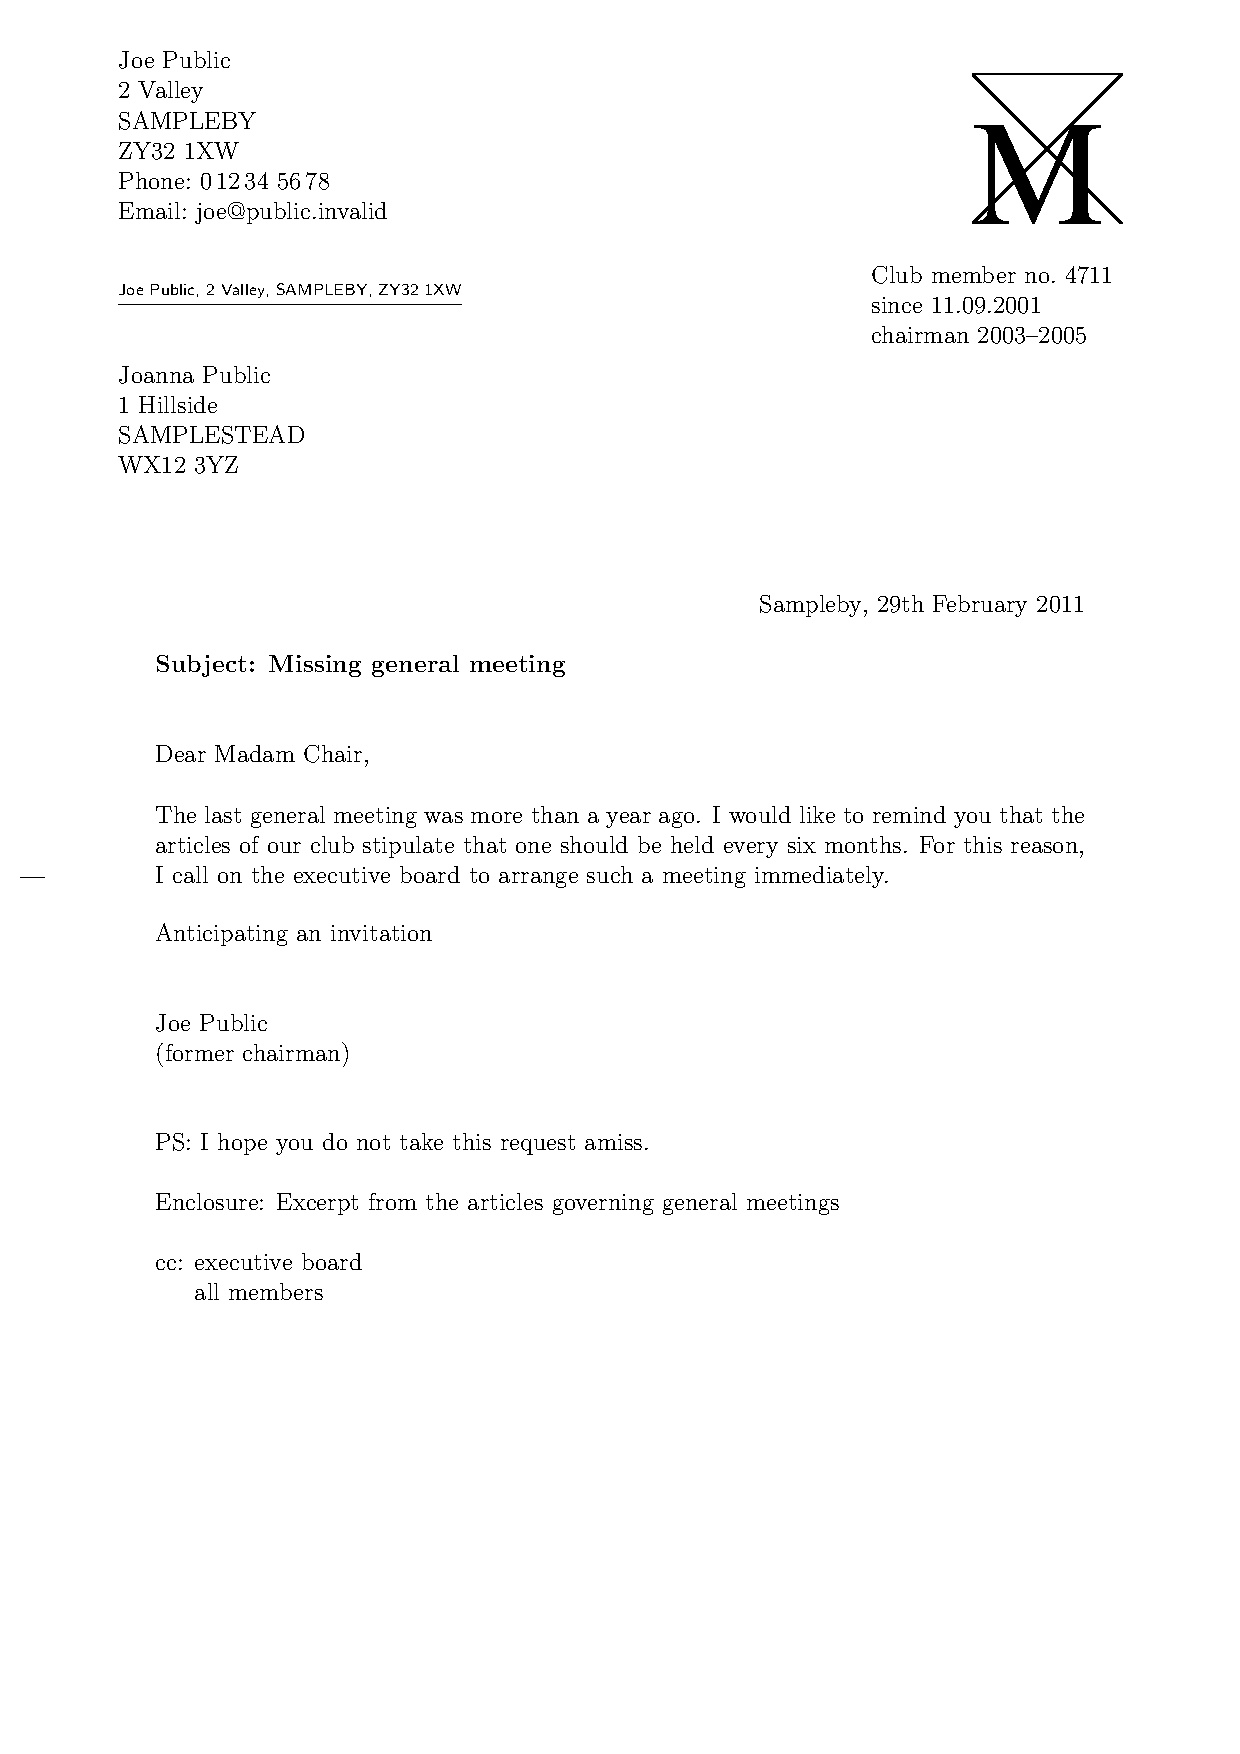
\includegraphics[width=.4\textwidth]{letter-example-23-en}}
    \end{captionbeside}
    \label{fig:\LabelBase.letter-23}
  \end{figure}
\end{Example}

Note\textnote{Attention!} that immediately after loading the document class,
normally neither a package for the input encoding nor a language package has
been loaded. Because of this, you should use \TeX's 7-bit encoding for all
non-ASCII characters. For example, use ``\Macro{ss}'' to produce a German
``\ss''.

In \autoref{tab:lcoFiles}, \autopageref{tab:lcoFiles} you can find a list of
all predefined \File{lco} files. If\textnote{Attention!} you use a printer
that has large unprintable areas on the left or right side, you might have
problems with the \Option{SN}\IndexOption{SN} option. Since the Swiss standard
SN~101\,130 stipulates that the address field should be placed 8\Unit{mm} from
the right edge of the paper, the headline and the sender attributes are also
placed at a correspondingly small distance from the paper edge. This also
applies to the reference line when using the
\DescRef{\LabelBase.option.refline}\PValue{=wide} option (see
\autoref{sec:\LabelBase.firstpage}, \DescPageRef{\LabelBase.option.refline}).
If\textnote{Hint!} you have this kind of problem, create your own \File{lco}
file that loads \Option{SN} first and then changes
\PLength{toaddrhpos}\IndexPLength{toaddrhpos} (see
\autoref{sec:\LabelBase.addressee},
\DescPageRef{\LabelBase.plength.toaddrvpos}) to a smaller value. In
addition, you should also reduce \PLength{toaddrwidth} accordingly.%

By\textnote{Hint!} the way, the \File{DIN} \File{lco} file is always loaded
automatically as the first \File{lco} file. This ensures that all
pseudo-lengths will have more or less reasonable default values. Therefore you
do not need to load this default file on your own.

With regard to the \File{lco} files \File{DIN5008A} and \File{DIN5008B}, it
should be noted that the corresponding regulations have certain leeway and, as
can be seen from various inquiries to the author, many users only wish to make
full use of these leeway, but also prefer one or the other deviation from the
standard. However, the two files implement only one interpretation of the
standard. The reader should therefore be reminded that these files are to be
understood only as templates, in order to facilitate the creation of own
adapted \File{lco} files.%
%
\begin{desclist}
  \renewcommand*{\abovecaptionskipcorrection}{-\normalbaselineskip}%
  \desccaption{%
    Predefined \File{lco} files\label{tab:lcoFiles}%
  }{%
    Predefined \File{lco} files (\emph{continued})%
  }%
  \oentry{DIN}{%
    \leavevmode%
    \IndexOption[indexmain]{DIN}\IndexFile[indexmain]{DIN.lco}%
    parameters for letters on A4 paper, complying with German standard
    DIN~676; suitable for window envelopes in the sizes C4, C5, C6, and C6/5
    (C6 long).}%
  \oentry{DINmtext}{%
    \leavevmode%
    \IndexOption[indexmain]{DINmtext}\IndexFile[indexmain]{DINmtext.lco}%
    parameters for letters on A4 paper, complying with DIN~676 but using an
    alternate layout with more text on the first page; only suitable for
    window envelopes in the sizes C6 and C6/5 (C6 long).}%
  \oentry{KakuLL}{%
    \leavevmode%
    \IndexOption[indexmain]{KakuLL}\IndexFile[indexmain]{KakuLL.lco}%
    parameters for Japanese letters on A4 paper; suitable for Japanese
    window envelopes of type Kaku A4, in which the window is approximately
    90\Unit{mm} wide by 45\Unit{mm} high, and positioned 25\Unit{mm} from the
    left and 24\Unit{mm} from the top edge (see \autoref{cha:japanlco}).}%
  \oentry{KOMAold}{%
    \leavevmode%
    \IndexOption[indexmain]{KOMAold}\IndexFile[indexmain]{KOMAold.lco}%
    parameters for letters on A4 paper using a layout close to that of the
    obsolete \Class{scrlettr} letter class; suitable for window envelopes in
    the sizes C4, C5, C6, and C6/5 (C6 long); some additional commands to
    improve compatibility with obsolete \Class{scrlettr} commands are defined;
    \Class{scrlttr2} may behave slightly differently with this \File{lco} file
    than with the other \File{lco} files.}%
  \oentry{NF}{%
    \leavevmode%
    \IndexOption[indexmain]{NF}\IndexFile[indexmain]{NF.lco}%
    parameters for French letters, complying with NF~Z~11-001; suitable for
    window envelopes of type DL (110\Unit{mm} by 220\Unit{mm}) with a window
    45\Unit{mm} wide by 100\Unit{mm} high placed about 20\Unit{mm} from the
    lower right edge; this file was originally developed by Jean-Marie
    Pacquet, who also provides LyX integration in addition to extensions at
    \cite{www:NF.lco}.}%
  \oentry{NipponEH}{%
    \leavevmode%
    \IndexOption[indexmain]{NipponEH}\IndexFile[indexmain]{NipponEH.lco}%
    parameters for Japanese letters on A4 paper; suitable for Japanese
    window envelopes of types Chou or You 3 or 4, in which the window is
    approximately 90\Unit{mm} wide by 55\Unit{mm} high, and positioned
    22\Unit{mm} from the left and 12\Unit{mm} from the top edge (see
    \autoref{cha:japanlco}).}%
  \oentry{NipponEL}{%
    \leavevmode%
    \IndexOption[indexmain]{NipponEL}\IndexFile[indexmain]{NipponEL.lco}%
    parameters for Japanese letters on A4 paper; suitable for Japanese
    window envelopes of types Chou or You 3 or 4, in which the window is
    approximately 90\Unit{mm} wide by 45\Unit{mm} high, and positioned
    22\Unit{mm} from the left and 12\Unit{mm} from the top edge (see
    \autoref{cha:japanlco}).}%
  \oentry{NipponLH}{%
    \leavevmode%
    \IndexOption[indexmain]{NipponLH}\IndexFile[indexmain]{NipponLH.lco}%
    parameters for Japanese letters on A4 paper; suitable for Japanese
    window envelopes of types Chou or You 3 or 4, in which the window is
    approximately 90\Unit{mm} wide by 55\Unit{mm} high, and positioned
    25\Unit{mm} from the left and 12\Unit{mm} from the top edge (see
    \autoref{cha:japanlco}).}%
  \oentry{NipponLL}{%
    \leavevmode%
    \IndexOption[indexmain]{NipponLL}\IndexFile[indexmain]{NipponLL.lco}%
    parameters for Japanese letters on A4 paper; suitable for Japanese
    window envelopes of types Chou or You 3 or 4, in which the window is
    approximately 90\Unit{mm} wide by 45\Unit{mm} high, and positioned
    25\Unit{mm} from the left and 12\Unit{mm} from the top edge (see
    \autoref{cha:japanlco}).}%
  \oentry{NipponRL}{%
    \leavevmode%
    \IndexOption[indexmain]{NipponRL}\IndexFile[indexmain]{NipponRL.lco}%
    parameters for Japanese letters on A4 paper; suitable for Japanese
    window envelopes of types Chou or You 3 or 4, in which the window is
    approximately 90\Unit{mm} wide by 45\Unit{mm} high, and positioned
    25\Unit{mm} from the left and 24\Unit{mm} from the top edge (see
    \autoref{cha:japanlco}).}%
  \oentry{SN}{%
    \leavevmode%
    \IndexOption[indexmain]{SN}\IndexFile[indexmain]{SN.lco}%
    parameters for Swiss letters with the address field on the right side,
    according to SN~010\,130; suitable for Swiss window envelopes in the sizes
    C4, C5, C6, and C6/5 (C6 long).}%
  \oentry{SNleft}{%
    \leavevmode%
    \IndexOption[indexmain]{SNleft}\IndexFile[indexmain]{SNleft.lco}%
    parameters for Swiss letters with the address field on the left side;
    suitable for Swiss window envelopes with the window on the left side in
    the sizes C4, C5, C6, and C6/5 (C6 long).}%
  \oentry{UScommercial9}{%
    \leavevmode%
    \IndexOption[indexmain]{UScommercial9}%
    \IndexFile[indexmain]{UScommercial9.lco}%
    parameters for US letters on American letter paper; suitable for
    \emph{commercial~No.\,9} US window envelopes with a window 4\,1/2\Unit{in}
    wide by 1\,1/8\Unit{in} high, positioned 7/8\Unit{in} from the left and
    1/2\Unit{in} from the bottom, without the return address inside the
    window; when folded first at the middle mark then at the top fold mark,
    legal paper can also be used but results in a paper-size warning}%
  \oentry{UScommercial9DW}{%
    \leavevmode%
    \IndexOption[indexmain]{UScommercial9DW}%
    \IndexFile[indexmain]{UScommercial9DW.lco}%
    parameters for US letters on American letter paper; suitable for
    \emph{commercial~No.\,9} US window envelopes with an recipient-address
    window 3\,5/8\Unit{in} wide by 1\,1/8\Unit{in} high, positioned
    3/4\Unit{in} from the left and 1/2\Unit{in} from the bottom, and with a
    return-address window 3\,1/2\Unit{in} wide by 7/8\Unit{in} high,
    positioned 5/16\Unit{in} from the left and 2\,1/2\Unit{in} from the
    bottom; when folded first at the middle mark and then at the top fold
    mark, legal paper can also be used but results in a paper-size warning}%
\end{desclist}
%
\EndIndexGroup
%
\EndIndexGroup


\section{Address Files and Form Letters}
\seclabel{addressFile}%
\BeginIndexGroup
\BeginIndex{}{address>file}%
\BeginIndex{}{form letters}%
\index{serial letters|see form letters}%
\index{circular letters|see form letters}%

One of the most annoying things about creating form letters is typing up
the different addresses. \KOMAScript{} provides basic support for this task%
\iffalse% Umbruchkorrekturtext
, as did its predecessor \Class{scrlettr}%
\fi%
.%
\iffalse% Umbruchkorrekturtext
\ Currently there are plans for greatly enhanced support.%
\fi

\begin{Declaration}
  \Macro{adrentry}\Parameter{last~name}\Parameter{first~name}%
  \Parameter{address}\Parameter{phone}\Parameter{F1}\Parameter{F2}%
  \Parameter{comment}\Parameter{key}
\end{Declaration}%
\Class{scrlttr2} and \Package{scrletter} can evaluate address files.
This can be very useful for form letters. An address file must have the
extension \File{.adr} and consists of a number \Macro{adrentry} entries.
An individual entry consists of eight parameters and may look, for example,
like this:
\begin{lstcode}
  \adrentry{McEnvy}
           {Flann}
           {1 High Street\\ Glasgow}
           {0141 123 4567}
           {builder}
           {}
           {buys everything}
           {FLANN}
\end{lstcode}
You can use the fifth and sixth elements, \PValue{F1} and \PValue{F2}, for
anything you want. Gender, academic grade, birth date, or the date the person
joined a society are all possibilities. The last parameter, \PName{key},
should consist of more than one letter and be upper-case only so as not to
interfere with existing \TeX{} or \LaTeX{} commands.

\begin{Example}
  Mr McEnvy is one of your most important business partners. Since you
  maintain a frequent correspondence with him, it is too tedious to
  enter all his data again and again. \KOMAScript{} will do this work for you.
  For example, if you have saved your customer contacts in the
  \File{partners.adr} address file and you would like to write a letter to
  Mr~McEnvy, you can save a great deal of effort by typing:
  \begin{lstcode}
    \input{partners.adr}
    \begin{letter}{\FLANN}
      Your correspondence of today \dots
    \end{letter}
  \end{lstcode}
  Please make sure that your {\TeX} system can access your address file.
  Otherwise the \Macro{input} command results in an error message. You can
  either put your address file in the same directory as your letter or
  configure your \TeX{} system to look for a dedicated address directory.
\end{Example}
% 
\EndIndexGroup


\begin{Declaration}
  \Macro{addrentry}\Parameter{last-name}\Parameter{first-name}%
  \Parameter{address}\Parameter{phone}\Parameter{F1}\Parameter{F2}%
  \Parameter{F3}\Parameter{F4}\Parameter{key}
\end{Declaration}%
Before you object that a total of two free parameters is too few,
\KOMAScript{} alternatively offers the \Macro{addrentry} command\,---\,note
the additional ``d''\,---\,which adds two more freely definable parameters but
omits the comment parameter. Otherwise, you can use this command in exactly
the same way as \DescRef{\LabelBase.cmd.adrentry}.

Both \DescRef{\LabelBase.cmd.adrentry} and \Macro{addrentry} commands can be
freely mixed in the \File{adr} files. I should note, however, that other
packages may not be designed to use \Macro{addrentry}. If necessary, you have
to create the appropriate extensions yourself.%
%
\EndIndexGroup

In addition to simplifying access to addresses, you can also use the
\File{adr} files to create circulars or form letters. Thus you can create such
mass mailings without a complicated connection to a database system.
%
\begin{Example}
  You want to sent a form letter to all members of your fishing club to invite
  them to the next general meeting.
\begin{lstcode}
  \documentclass{scrlttr2}
  \begin{document}
  \renewcommand*{\adrentry}[8]{%
    \begin{letter}{#2 #1\\#3}
      \opening{Dear members,}
      Our next general meeting will be on
      Monday, 12 August 2002.
      
      The following topics are \dots
      \closing{Regards,}
    \end{letter}
  }
  \input{members.adr}
  \end{document}
\end{lstcode}
  If the address file also contains \DescRef{\LabelBase.cmd.addrentry}
  commands, you must add a corresponding definition before loading the address
  file:
\begin{lstcode}
  \renewcommand*{\addrentry}[9]{%
    \adrentry{#1}{#2}{#3}{#4}{#5}{#6}{#7}{#9}%
  }
\end{lstcode}
  In this example, the extra freely-definable parameter is not used, and
  therefore \DescRef{\LabelBase.cmd.addrentry} is defined using
  \DescRef{\LabelBase.cmd.adrentry}.
\end{Example}

Of course, the letter's contents can also be adapted to the characteristics of
the address data. You can use the free parameters of the
\DescRef{\LabelBase.cmd.adrentry} and \DescRef{\LabelBase.cmd.addrentry}
commands for this.
\begin{Example}
  Suppose you use the fifth parameter of the \DescRef{\LabelBase.cmd.adrentry}
  command to indicate the gender of a club member (\PValue{m/f}), and the
  sixth parameter to indicate the amount of membership dues that is unpaid.
  If you would like to write a reminder to each such member and address them
  personally, the next example will help you:
\begin{lstcode}
  \renewcommand*{\adrentry}[8]{
    \ifdim #6pt>0pt\relax
    % #6 is an amount (floating-point number) greater than 0.
    % Thus, this selects all members owing dues.
      \begin{letter}{#2 #1\\#3}
        \if #5m \opening{Dear Mr #2,} \fi
        \if #5f \opening{Dear Ms #2,} \fi

        Unfortunately, we have noticed that you are in arrears
        with the payment of your membership fees.

        Please remit the outstanding balance of \pounds #6 to the club
        account.
       \closing{Regards,}
      \end{letter}
     \fi
  }
\end{lstcode}
\end{Example}
It is therefore possible to tailor the text of the letter to the specific
characteristics of the recipient and create the impression of a personal
letter. The extent of the customisation is only limited by the maximum number
of two free \DescRef{\LabelBase.cmd.adrentry} parameters and four free
\DescRef{\LabelBase.cmd.addrentry} parameters.


\begin{Declaration}
  \Macro{adrchar}\Parameter{initial letter}%
  \Macro{addrchar}\Parameter{initial letter}
\end{Declaration}
\Index[indexmain]{address>list}\Index[indexmain]{telephone directory}%
It is possible to create address lists and telephone directories using
\File{adr} files. You also need the \Package{adrconv}\IndexPackage{adrconv}
package by Axel Kielhorn (see \cite{package:adrconv}). This package contains
interactive \LaTeX{} documents which make it easy to create such lists.

The address files have to be sorted already in order to obtain sorted lists.
It is advisable to insert an \Macro{adrchar} or \Macro{addrchar} command
containing the initial letter of the \PName{last name} before the point in the
list where this letter changes. \Class{scrlettr2} and \Package{scrletter} will
ignore these commands.
%
\begin{Example}
  Suppose you have the following, rather tiny address file from which you
  want to create an address book:
\begin{lstlisting}
  \adrchar{A}
  \adrentry{Angel}{Gabriel}
           {Cloud 3\\12345 Heaven's Realm}
           {000\,01\,02\,03}{}{}{archangel}{GABRIEL}
  \adrentry{Angel}{Michael}
           {Cloud 3a\\12345 Heaven's Realm}
           {000\,01\,02\,04}{}{}{archangel}{MICHAEL}
  \adrchar{K}
  \adrentry{Kohm}{Markus}
           {Freiherr-von-Drais-Stra\ss e 66\\68535 Edingen-Neckarhausen}
           {+49~62\,03~1\,??\,??}{}{}{no angel at all}
           {KOMA}
\end{lstlisting}
  You can now process these entries using the \File{adrdir.tex} document from
  \cite{package:adrconv}. The result looks something like this:
  \begin{center}
    \setlength{\unitlength}{1mm}
    \begin{picture}(80,57)
      \put(0,57){\line(1,0){80}}
      \put(0,3){\line(0,1){54}}
      \put(80,3){\line(0,1){54}}
      \thicklines
      \put(10,42){\line(1,0){60}}
      \put(70,45){\makebox(0,0)[r]{\textsf{\textbf{A}}}}
      \put(10,23){\makebox(0,20)[l]{\parbox{5cm}{\raggedright
            \textsc{Angel}, Gabriel\\\quad\small Cloud 3\\
            \quad 12345 Heaven's Realm\\
            \quad (archangel)}}}
      \put(70,23){\makebox(0,20)[r]{\parbox{2cm}{\raggedright~\\
            \small~\\\textsc{gabriel}\\000\,01\,02\,03}}}
      \put(10,4){\makebox(0,20)[l]{\parbox{5cm}{\raggedright
            \textsc{Angel}, Michael\\\quad\small Cloud 3a\\
            \quad 12345 Heaven's Realm\\
            \quad (archangel)}}}
      \put(70,4){\makebox(0,20)[r]{\parbox{2cm}{\raggedright~\\
            \small~\\\textsc{michael}\\000\,01\,02\,04}}}
      \qbezier(0,3)(10,6)(40,3)\qbezier(40,3)(60,0)(80,3)
    \end{picture}
  \end{center}
  The letter in the header is generated by answering ``no'' to the
  question ``Names in the header?'' See explanation in \File{adrdir.tex}.
\end{Example}

Package \Package{adrconv}\IndexPackage{adrconv} can also be used to create
address files compatible with the \KOMAScript{} letter class or package or
with the \Package{scraddr} package from an address database in \BibTeX{}
format containing entries like:
\begin{lstlisting}[morekeywords={@address}]
  @address{HMUS,
     name =      {Carl McExample},
     title =     {Dr.},
     city =      {Anywhere},
     zip =       01234,
     country =   {Great Britain},
     street =    {A long Road},
     phone =     {01234 / 5 67 89},
     note =      {always forget his birthday},
     key =       {HMUS},
  }
\end{lstlisting}
You can find more about the \Package{adrconv}\IndexPackage{adrconv} package in
its documentation.%
%
\EndIndexGroup
%
\EndIndexGroup
%
\EndIndexGroup

\endinput

%%% Local Variables: 
%%% mode: latex
%%% TeX-master: "scrguide-en.tex"
%%% coding: utf-8
%%% ispell-local-dictionary: "en_GB"
%%% eval: (flyspell-mode 1)
%%% End: 
